\documentclass[a4paper,11pt]{article}
% --- Kodowanie / języki (w PDFLaTeX) ---
\usepackage[utf8]{inputenc}
\usepackage[T1]{fontenc}
\usepackage[english,polish]{babel} % polski jako drugi -> zwykle i tak wybierasz \selectlanguage
% \usepackage{polski} % ZAZWYCZAJ zbędne przy babel+polish; zostaw tylko jeśli masz konkretne powody

% --- Marginesy ---
\usepackage[margin=2.5cm]{geometry} % prościej niż hmargin+height

% --- Fonty ---
\usepackage{helvet}
\renewcommand{\familydefault}{\sfdefault} % jeśli chcesz cały dokument sans-serif
% Jeśli NIE chcesz całego dokumentu sans-serif, usuń linię wyżej i używaj \textsf{} lokalnie.

% --- Matematyka ---
\usepackage{amsmath,amssymb,amsfonts}

% --- Grafika / rysunki ---
\usepackage{graphicx}
\usepackage{epstopdf} % tylko jeśli faktycznie używasz EPS
\usepackage{tikz}
\usepackage{url} % for \url in bibliography
\usetikzlibrary{positioning,arrows.meta}

% -------------------------------------------------
% Rysunki i podpisy
% -------------------------------------------------
\usepackage{graphicx}
\usepackage{float}
\usepackage{caption}

\captionsetup{
  font=small,
  labelfont=bf,
  labelsep=space,
  figurename=Rys.
}

% --- Tabele / układ ---
\usepackage{booktabs}
\usepackage{multirow}
\usepackage{multicol}
\usepackage{float}

% --- Kolory / linki ---
\usepackage{xcolor}
\usepackage{url}
\usepackage[hidelinks]{hyperref}

% --- Bibliografia ---
\usepackage[numbers]{natbib}

% --- Listy ---
\usepackage{enumitem}
\setlist{nosep}
\raggedbottom

% --- Podpisy i subfigury ---
\usepackage{caption}
\usepackage{subcaption}

% --- Kod źródłowy ---
\usepackage{listings}
\lstset{
  basicstyle=\ttfamily\small,
  backgroundcolor=\color{gray!10},
  frame=single,
  breaklines=true,
  numbers=left,
  numberstyle=\tiny\color{gray},
  keywordstyle=\color{blue},
  commentstyle=\color{green!50!black},
  stringstyle=\color{red!70!black},
  showstringspaces=false,
  literate={ą}{{\k{a}}}1 {ć}{{\'c}}1 {ę}{{\k{e}}}1 {ł}{{\l{}}}1 {ń}{{\'n}}1 {ó}{{\'o}}1 {ś}{{\'s}}1 {ź}{{\'z}}1 {ż}{{\.z}}1
           {Ą}{{\k{A}}}1 {Ć}{{\'C}}1 {Ę}{{\k{E}}}1 {Ł}{{\L{}}}1 {Ń}{{\'N}}1 {Ó}{{\'O}}1 {Ś}{{\'S}}1 {Ź}{{\'Z}}1 {Ż}{{\.Z}}1
}

% --- Nagłówki stron ---
\usepackage{fancyhdr}
\pagestyle{fancy}
\fancyhf{}
\fancyhead[L]{Opracowanie}
\fancyhead[R]{\thepage}
\renewcommand{\headrulewidth}{0.4pt}

% --- Microtypografia (automatyczna korekta overfull/underfull) ---
\usepackage[protrusion=true,expansion=false]{microtype}

% --- Interlinia ---
\usepackage{setspace}
\onehalfspacing

% --- Spis treści (opcjonalnie, jeśli faktycznie modyfikujesz TOC) ---
\usepackage{tocloft}

% --- Unicode znaki (żeby LaTeX nie krzyczał) ---
\usepackage{newunicodechar}
\newunicodechar{₂}{$_2$}
\newunicodechar{₃}{$_3$}
\newunicodechar{α}{$\alpha$}
\newunicodechar{β}{$\beta$}
\newunicodechar{γ}{$\gamma$}
\newunicodechar{σ}{$\sigma$}
\newunicodechar{ε}{$\varepsilon$}
\newunicodechar{φ}{$\varphi$}
\newunicodechar{→}{$\rightarrow$}
\newunicodechar{×}{$\times$}

% =====================================================
%  WYGLĄD NAGŁÓWKÓW + NUMERACJA DO POZIOMU 2
% =====================================================
\usepackage{titlesec}

% Numeruj: section (1), subsection (2), subsubsection (3). Paragraph (4) bez numeru.
\setcounter{secnumdepth}{3}
% W spisie treści pokaż do subsubsection (opcjonalnie):
\setcounter{tocdepth}{3}

% SECTION Poziom 0: wyraźny (większy, półgruby)
\titleformat{\section}
  {\normalfont\Large\bfseries\sffamily}
  {\thesection}{1em}{}

% SUBSECTION Poziom 1: trochę mniejszy, nadal wyraźny
\titleformat{\subsection}
  {\normalfont\large\bfseries\sffamily}
  {\thesubsection}{1em}{}

% SUBSUBSECTION Poziom 2: bez pogrubienia (żeby nie było "wszędzie grubo"), ale np. italik + trochę odstępu
\titleformat{\subsubsection}
  {\normalfont\bfseries\normalsize\sffamily}
  {\thesubsubsection}{1em}{}

% PARAGRAPH Poziom 3: jako osobna linia (block), BEZ numeru i bez przesadnego bolda
\titleformat{\paragraph}[block]
  {\normalfont\bfseries\normalsize\sffamily}
  {}{0em}{}

% Odstępy: różnicują poziomy bardziej niż sama czcionka
\titlespacing*{\section}{0pt}{2.5ex plus 1ex minus .2ex}{1.2ex}
\titlespacing*{\subsection}{0pt}{2.0ex plus 0.8ex minus .2ex}{0.9ex}
\titlespacing*{\subsubsection}{0pt}{1.5ex plus 0.6ex minus .2ex}{0.6ex}
\titlespacing*{\paragraph}{0pt}{1.0ex plus 0.4ex minus .2ex}{0.4ex}

% =====================================================
%  Tytułowa
% =====================================================
\newcommand{\setFaculty}[1]{\newcommand{\faculty}{#1}}
\newcommand{\setDepartment}[1]{\newcommand{\department}{#1}}
\newcommand{\setSupervisor}[1]{\newcommand{\supervisor}{#1}}
\newcommand{\setTitleang}[1]{\newcommand{\Titleang}{#1}}
\newcommand{\setMajor}[1]{\newcommand{\major}{#1}}
\newcommand{\setWorkType}[1]{\newcommand{\worktype}{#1}}
\newcommand{\setPlaceYear}[1]{\newcommand{\placeyear}{#1}}

\makeatletter
\renewcommand{\maketitle}{%
\begin{titlepage}
  \thispagestyle{empty}

  \begin{center}
    % Preferuj PDF (wektor). Jeśli nie ma, użyj JPG.
    \IfFileExists{img/logo_AGH.pdf}
      {
\includegraphics[width=\textwidth]{img/00_title/logo_AGH.jpg}}
      {
\includegraphics[width=\textwidth]{img/00_title/logo_AGH.jpg}}\\[2mm]

    {\bf\sf \MakeUppercase{\faculty}}\\[5mm]
    {\bf\sf \MakeUppercase{\department}}\\[14mm]

    {\sf\huge \worktype}\\[12mm]

    {\sf\Large
      \@title \par\vspace{5mm}
      \Titleang
    }\\[30mm]
  \end{center}

  {\sf
  \noindent
  \begin{tabular}{ll}
    Autor: & \@author\\
    Kierunek studiów: & \major\\
    Opiekun pracy: & \supervisor\\
  \end{tabular}
  }

  \vspace{10mm}
  \begin{center}
    {\sf \placeyear}
  \end{center}

\end{titlepage}
}
\makeatother


%% ================================================== %%
%%                 STRUKTURA RODZIAŁÓW                %%
%% ================================================== %%
%%                                                    %%
%%   \section{Nagłówek sekcji}                        %%
%%   \label{sec:Nagłówek sekcji}                      %%
%%                                                    %%
%%   \subsection{Poziom 1}                            %%
%%                                                    %%
%%   \subsubsection{Poziom 2}                         %%
%%                                                    %%
%%   \paragraph{Poziom 3}\mbox{}\\                    %%
%% ================================================== %%

% --- TU WPISZ IMIĘ I NAZWISKO -----
\author{Rafał Zabłotni}

% --- TU WPISZ TYTUŁ PRACY (PL)
\title{Wykorzystanie technik DevOps w implementacji automatycznego procesu CI/CD do uczenia i wersjonowania modeli sztucznej inteligencji: analiza utrzymania systemów wykorzystujących sztuczną inteligencję w porównaniu do metod manualnych}

% --- TU WPISZ TYTUŁ PRACY (EN)
\setTitleang{Using DevOps techniques to implement an automated CI/CD process for training and versioning AI models: an analysis of the maintenance of AI-based systems compared to manual methods}

% --- TU WPISZ KIERUNEK STUDIÓW
\setMajor{Inżynieria Obliczeniowa}

% --- Jednostki
\setFaculty{Wydział Inżynierii Metali i Informatyki Przemysłowej}
\setDepartment{Katedra Informatyki Stosowanej i Modelowania}

% --- Opiekun
\setSupervisor{mgr inż. Piotr Hajder}

% --- Rodzaj pracy (Projekt dyplomowy / Praca dyplomowa)
\setWorkType{Projekt dyplomowy}

% --- Miasto i rok
\setPlaceYear{Kraków, 2026}

\begin{document}
\pagestyle{empty}
\maketitle

\pagestyle{plain}

\newpage
\pagenumbering{arabic}
\tableofcontents
\newpage

\section{Wstęp}

\subsection{Geneza}

Pomysł na realizację niniejszego projektu zrodził się podczas analizowania wysokopoziomowych testów modułowych. Wspomniane testy charakteryzują się wysokim poziomem abstrakcji oraz szerokim zakresem funkcjonalności, co skutkuje dużą liczbą wymaganych powtarzalnych ustawień. Na tej podstawie zaobserwowano interesującą tendencję polegającą na tym, że znaczna część kodu testowego okazywała się redundantna, a wiele mechanizmów było wielokrotnie powielanych poprzez kopiowanie oraz wprowadzanie drobnych modyfikacji do istniejących fragmentów kodu.

Naturalnym rozwiązaniem tego problemu mogłoby wydawać się wydzielanie powtarzalnych elementów do funkcji pomocniczych lub bibliotek testowych oraz utrzymywanie ich w uporządkowanej i współdzielonej formie. Podejście to jednak wiąże się z istotnymi trudnościami, zarówno natury organizacyjnej, jak i technicznej. W praktyce często prowadzi ono do nadmiernego rozrostu bibliotek pomocniczych, niejednoznacznych interfejsów oraz problemów z ich długoterminowym utrzymaniem.

W szczególności pojawiają się następujące problemy:
\begin{enumerate}
  \item Jak określić moment, w którym dana funkcjonalność jest wystarczająco generyczna, aby mogła zostać wydzielona do wspólnej biblioteki?
  \item Jak zminimalizować ryzyko tworzenia funkcji lokalnie w plikach testowych, które z czasem zaczynają być wykorzystywane przez inne testy, prowadząc do niejawnych zależności pomiędzy teoretycznie niezależnymi modułami?
  \item Jak zapewnić spójny sposób tworzenia oraz utrzymania takich funkcji w projektach rozwijanych przez dziesiątki, a niekiedy setki programistów, o różnym poziomie doświadczenia i odmiennych nawykach pracy?
\end{enumerate}

Jednocześnie, jak powszechnie wiadomo, modele sztucznej inteligencji uczą się na podstawie zbiorów danych treningowych, a następnie wykorzystują wyuczone wzorce do rozwiązywania nowych problemów. Obserwacja ta stała się punktem wyjścia do rozważenia możliwości zastosowania modeli sztucznej inteligencji (ang. Artificial Intelligence, AI) w obszarze automatycznego generowania wspólnych, powtarzalnych fragmentów kodu testowego na podstawie już istniejących przykładów.

Jednakże, aby taki system mógł zostać efektywnie wdrożony w praktyce, niezbędne jest zaprojektowanie i utrzymanie procesu ciągłej integracji i ciągłego dostarczania (ang. Continuous Integration / Continuous Delivery, CI/CD), zapewniającego automatyczne trenowanie modeli, ich ewaluację oraz kontrolowane wdrażanie w środowisku produkcyjnym. W przeciwnym razie konieczne byłoby wyznaczenie osoby odpowiedzialnej za manualne utrzymanie i nadzór.

W ten sposób wyłaniają się dwa kluczowe pytania stanowiące oś niniejszego projektu:
\begin{enumerate}
\item Czy stworzenie modelu AI umożliwiającego automatyczne generowanie fragmentów kodu testowego jest rozwiązaniem możliwym do realizacji oraz uzasadnionym ekonomicznie?
\item Czy bardziej opłacalne jest oddelegowanie pracownika do ręcznego utrzymywania i rozwijania tego rozwiązania, czy też zasadne jest jego zautomatyzowanie z wykorzystaniem narzędzi DevOps oraz procesów CI/CD?
\end{enumerate}

\subsection{Założenia}

Ze względu na złożoność problemu generowania kodu testowego oraz ograniczony czas realizacji projektu zdecydowano się na zastosowanie problemu zastępczego, umożliwiającego weryfikację postawionej hipotezy bez konieczności budowania zaawansowanego modelu językowego. Jako problem zastępczy wybrano segmentację semantyczną obrazów wodomierzy z wykorzystaniem architektury U-Net. Wybór ten jest uzasadniony, ponieważ modele segmentacyjne posiadają jednoznacznie zdefiniowane metryki jakości, takie jak współczynnik Dice (ang. Dice coefficient, miara nakładania masek) oraz IoU (ang. Intersection over Union, stosunek części wspólnej do sumy obszarów), charakteryzują się umiarkowanymi wymaganiami obliczeniowymi umożliwiającymi trening w ramach dostępnego budżetu, a także opierają się na dostępnych modelach wstępnie wytrenowanych, co pozwala na obiektywne porównanie kolejnych wersji.

Dla uproszczenia przyjęto założenie, że model sztucznej inteligencji dostarczany jest przez zewnętrzną firmę, natomiast zakres pracy obejmuje jego dalsze uczenie, ocenę jakości oraz wdrażanie. Takie podejście odzwierciedla realny scenariusz środowiska produkcyjnego, w którym zespół DevOps otrzymuje gotowy model i odpowiada za zarządzanie jego cyklem życia.

W tak zdefiniowanym kontekście drugie pytanie sformułowane w poprzedniej sekcji pozostaje aktualne: czy bardziej opłacalne jest oddelegowanie pracownika do ręcznego utrzymywania i rozwijania tego rozwiązania, czy też zasadne jest jego zautomatyzowanie z wykorzystaniem narzędzi DevOps oraz procesów CI/CD? W podejściu manualnym proces ponownego uczenia i wdrażania modelu obejmuje ręczne przygotowanie danych, uruchamianie treningu, walidację wyników oraz publikację nowej wersji. Podejście to, mimo swojej prostoty koncepcyjnej, wiąże się z ryzykiem błędów ludzkich, trudnościami w zachowaniu powtarzalności eksperymentów oraz ograniczoną skalowalnością. Automatyzacja natomiast umożliwia jednoznaczne powiązanie wersji modelu z wersją danych treningowych, wprowadzenie obiektywnej bramki jakości oraz eliminację ręcznych etapów mogących prowadzić do niespójności.

W ramach niniejszej pracy opracowano kompletny, zautomatyzowany system CI/CD dla modeli sztucznej inteligencji. System obejmuje wersjonowanie danych treningowych z wykorzystaniem narzędzia DVC, śledzenie eksperymentów i rejestr modeli (MLflow), automatyczny potok (and. pipeline) treningowy uruchamiany w GitHub Actions, mechanizm bramki jakości porównujący nowy model z aktualną wersją produkcyjną oraz wdrożenie modelu w środowisku chmurowym za pomocą lekkiej dystrybucji Kubernetes (k3s), uruchomionej na instancji Amazon EC2  (ang. Elastic Compute Cloud, Elastyczna Chmura Obliczeniowa) wraz z mechanizmami monitoringu (Prometheus, Grafana). Całość zaprojektowano w taki sposób, aby dodanie nowych danych treningowych wymagało jedynie wykonania polecenia \texttt{git push}, a pozostałe etapy procesu przebiegały automatycznie. Tak zdefiniowany zakres umożliwia bezpośrednie porównanie kosztów i nakładu pracy podejścia manualnego oraz zautomatyzowanego, co stanowi główny cel analityczny pracy.

\section{Wprowadzenie Teoretyczne}

Realizacja projektu opisanego w niniejszej pracy opiera się na zestawie technologii i koncepcji z obszaru inżynierii oprogramowania, uczenia maszynowego i infrastruktury chmurowej. Niniejszy rozdział przedstawia teoretyczne podstawy każdego z tych elementów, stanowiąc punkt odniesienia dla decyzji projektowych opisanych w kolejnych rozdziałach. Omówiono kolejno: filozofię DevOps i mechanizmy CI/CD, podejście MLOps jako ich rozszerzenie na świat modeli ML, a następnie konkretne narzędzia zastosowane w projekcie: Git i GitHub, GitHub Actions, Docker, Kubernetes (k3s), Terraform z Helm, MLflow, DVC oraz Prometheus z Grafaną.

\subsection{DevOps}

DevOps to zbiór praktyk, kultury organizacyjnej i narzędzi, których celem jest skrócenie cyklu życia oprogramowania przy jednoczesnym zapewnieniu wysokiej jakości dostarczanych produktów. Termin pochodzi od połączenia słów \textit{Development} i \textit{Operations}, co odzwierciedla dążenie do przełamania tradycyjnej bariery między zespołami deweloperskimi a operacyjnymi.

Kluczowym elementem filozofii DevOps jest pętla ciągłego doskonalenia, obejmująca planowanie, kodowanie, budowanie, testowanie, wdrażanie, uruchamianie oraz monitorowanie. Każdy obrót pętli dostarcza informacje zwrotne, które pozwalają szybciej reagować na błędy i wymagania użytkowników. W kontekście niniejszej pracy DevOps stanowi ramy koncepcyjne, w których osadzony jest cały projekt - automatyzacja procesu trenowania i wdrażania modelu SI jest bezpośrednią aplikacją tych zasad \cite{loukides_devops_bookey}.

\subsection{Ciągła Integracja i Ciągłe Dostarczanie (CI/CD)}

Ciągła Integracja (ang. \textit{Continuous Integration}, CI) polega na automatycznym scalaniu i weryfikacji zmian kodu wielokrotnie w ciągu dnia. Każda zmiana uruchamia zdefiniowany zestaw testów, co pozwala wykryć błędy integracyjne natychmiast po ich wprowadzeniu, zamiast odkrywać je dopiero na etapie wydania.

Ciągłe Dostarczanie (ang. \textit{Continuous Delivery}) rozszerza CI o automatyczne przygotowanie artefaktów gotowych do wdrożenia. Ciągłe Wdrażanie (ang. \textit{Continuous Deployment}) idzie krok dalej - każda zmiana spełniająca kryteria jakości jest wdrażana do produkcji.

\begin{figure}[H]
  \centering
  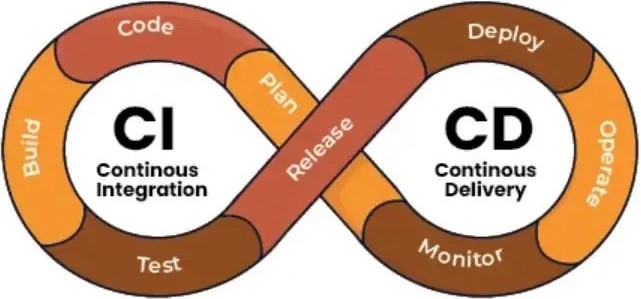
\includegraphics[width=0.55\linewidth]{img/02_wprowadzenie_teoretyczne/CI-CD.jpg}
  \caption{Przykład flow CI/CD \cite{geeksforgeeks_cicd}.}
\end{figure}

Typowy pipeline CI/CD składa się z następujących etapów:
\begin{enumerate}
  \item weryfikacja kodu (linting, testy jednostkowe),
  \item budowanie artefaktów (np. obrazu Docker),
  \item testy integracyjne i akceptacyjne,
  \item wdrożenie na środowisko docelowe,
  \item weryfikacja po wdrożeniu (smoke tests).
\end{enumerate}

\subsection{MLOps}

MLOps (ang. \textit{Machine Learning Operations}) to dyscyplina stosująca zasady DevOps do specyfiki cyklu życia modeli uczenia maszynowego. W odróżnieniu od klasycznego oprogramowania, gdzie artefaktem jest kod, w ML artefaktem jest model --- wynik trenowania na konkretnym zbiorze danych. To wprowadza kilka dodatkowych wyzwań:

\begin{itemize}
  \item dane treningowe zmieniają się niezależnie od kodu,
  \item wyniki trenowania są niedeterministyczne,
  \item jakość modelu musi być mierzona obiektywnie przed każdym wdrożeniem,
  \item modele degradują się w czasie (tzw. \textit{data drift}).
\end{itemize}

\begin{figure}[H]
  \centering
  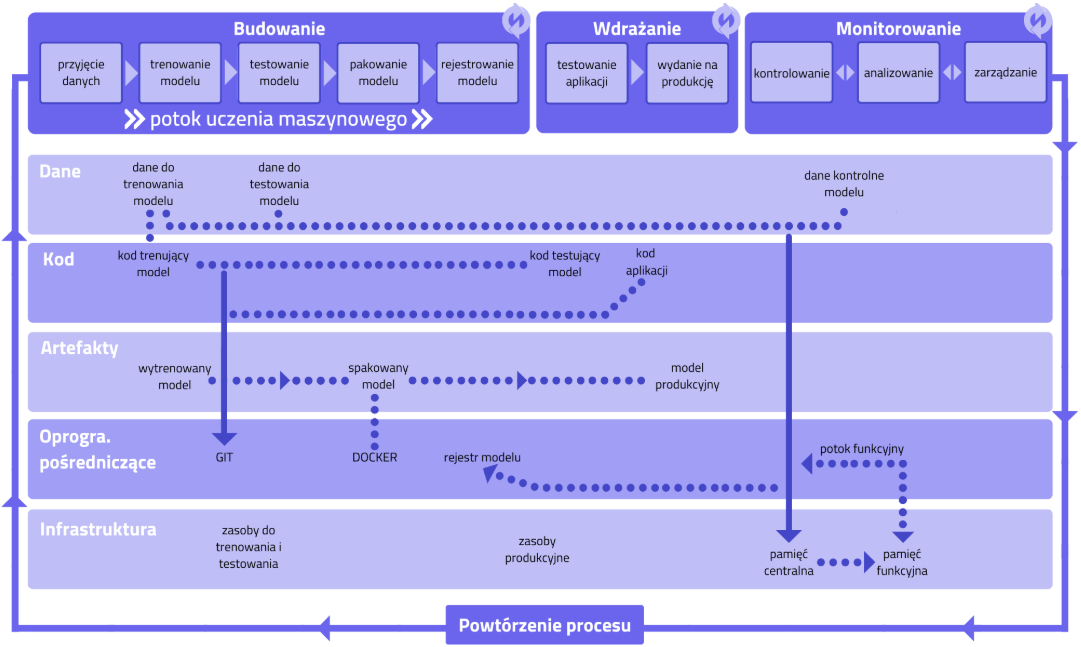
\includegraphics[width=\linewidth]{img/02_wprowadzenie_teoretyczne/mlops_flow.png}
  \caption{Przykład flow CI/CD \cite{mlops_flow}.}
\end{figure}

MLflow spina cały cykl życia modelu ML — od rejestrowania eksperymentów, parametrów i metryk podczas treningu, przez wersjonowanie oraz rejestrację modeli w Model Registry, aż po zarządzanie wdrożeniem i monitorowanie kolejnych wersji w środowisku produkcyjnym.
\subsection{Kontrola wersji --- Git i GitHub}

Git to rozproszony system kontroli wersji, będący de facto standardem w nowoczesnym tworzeniu oprogramowania \cite{chacon2014pro_git}. Przechowuje pełną historię zmian w postaci grafu migawek (ang. \textit{snapshots}), umożliwiając równoległą pracę na gałęziach (ang. \textit{branches}), scalanie zmian oraz cofanie się do dowolnego punktu w historii projektu.

Kluczowe koncepcje Gita:
\begin{itemize}
  \item \textbf{Commit} --- migawka stanu repozytorium w danym momencie wraz z metadanymi (autor, czas, wiadomość),
  \item \textbf{Branch} --- niezależna linia rozwoju; umożliwia pracę nad funkcjonalnością bez wpływu na gałąź główną,
  \item \textbf{Merge / Pull Request} --- scalenie zmian z jednej gałęzi do drugiej, zazwyczaj poprzedzone przeglądem kodu,
  \item \textbf{Hook} --- skrypt uruchamiany automatycznie w odpowiedzi na zdarzenie Gita (np. \texttt{pre-push}).
\end{itemize}

GitHub to platforma hostingowa dla repozytoriów Git, rozbudowana o funkcje współpracy zespołowej: pull requesty, przeglądy kodu, zarządzanie zadaniami oraz zintegrowane CI/CD w postaci GitHub Actions. W kontekście niniejszego projektu GitHub pełni rolę centralnego punktu integracji --- każda zmiana przechodzi przez repozytorium i może automatycznie uruchamiać kolejne etapy pipeline'u.

\subsection{GitHub Actions}

GitHub Actions to platforma automatyzacji wbudowana w GitHub, pozwalająca definiować przepływy pracy (ang. \textit{workflows}) jako pliki YAML przechowywane bezpośrednio w repozytorium \cite{github_actions_docs}. Workflow uruchamiane są w odpowiedzi na zdarzenia: push, pull request, harmonogram (cron) lub wywołanie ręczne.

Podstawowe pojęcia:
\begin{itemize}
  \item \textbf{Workflow} --- zestaw automatycznych zadań zdefiniowany w pliku \texttt{.github/workflows/*.yaml},
  \item \textbf{Job} --- jednostka wykonania złożona z kroków (steps); domyślnie uruchamiana równolegle z innymi jobami,
  \item \textbf{Step} --- pojedyncza operacja w ramach joba: wywołanie skryptu lub gotowej akcji,
  \item \textbf{Runner} --- maszyna wykonująca joba; może być zarządzana przez GitHub (hosted) lub przez użytkownika (self-hosted),
  \item \textbf{Artefakt} --- plik lub katalog przekazywany między jobami albo pobierany po zakończeniu workflow.
\end{itemize}

Kluczową cechą GitHub Actions jest możliwość użycia \textbf{self-hosted runners} --- maszyn zarządzanych przez użytkownika, co w niniejszym projekcie pozwala uruchamiać trening bezpośrednio na instancji EC2 wyposażonej w odpowiedni sprzęt obliczeniowy, bez potrzeby przekazywania danych treningowych przez sieć do zewnętrznego runnera.

\subsection{Konteneryzacja --- Docker}

Docker to platforma do tworzenia, dystrybucji i uruchamiania aplikacji w kontenerach \cite{merkel2014docker}. Kontener to izolowane środowisko uruchomieniowe zawierające aplikację wraz ze wszystkimi jej zależnościami: bibliotekami, interpreterem, zmiennymi środowiskowymi. Dzięki temu aplikacja działa identycznie na maszynie dewelopera, serwerze testowym i produkcji, eliminując problem \textit{,,u mnie działa''}.

Kluczowe pojęcia:
\begin{itemize}
  \item \textbf{Obraz (image)} --- niezmienialny szablon opisujący środowisko, definiowany plikiem \texttt{Dockerfile},
  \item \textbf{Kontener} --- działająca instancja obrazu; izolowana od systemu hosta i innych kontenerów,
  \item \textbf{Rejestr (registry)} --- repozytorium obrazów (np. Docker Hub, Amazon ECR).
\end{itemize}

W projekcie Docker służy do pakowania API modelu oraz do zapewnienia powtarzalności środowiska treningowego. Obraz z modelem jest budowany automatycznie w pipeline po zatwierdzeniu nowej wersji modelu.

\subsection{Kubernetes i k3s}

Kubernetes (K8s) to system do orkiestracji kontenerów --- automatyzuje ich wdrażanie, skalowanie i zarządzanie \cite{burns2016borg}. Zamiast uruchamiać kontenery ręcznie na konkretnych maszynach, Kubernetes przyjmuje deklaratywny opis pożądanego stanu (ile replik, jakie zasoby, jak reagować na awarie) i utrzymuje ten stan niezależnie od zdarzeń infrastrukturalnych.

k3s to uproszczona dystrybucja Kubernetes stworzona przez Rancher Labs. Zmniejsza wymagania sprzętowe (minimalna instalacja działa na instancji z 2~GB RAM) i upraszcza instalację do pojedynczego polecenia. Jest przeznaczona dla środowisk brzegowych, IoT oraz małych klastrów. W niniejszym projekcie k3s zainstalowany na pojedynczej instancji EC2 zastępuje zarządzany klaster EKS, co pozwala ograniczyć koszty do minimum.

\subsection{Infrastruktura jako kod --- Terraform i Helm}

\textbf{Infrastruktura jako kod} (ang. \textit{Infrastructure as Code}, IaC) to praktyka definiowania i zarządzania zasobami infrastrukturalnymi za pomocą plików konfiguracyjnych przechowywanych w systemie kontroli wersji, zamiast ręcznego konfigurowania przez interfejs graficzny lub CLI \cite{hashicorp_terraform}. Dzięki temu środowisko jest powtarzalne, audytowalne i odtwarzalne dowolnym momencie.

\textbf{Terraform} to narzędzie IaC firmy HashiCorp umożliwiające tworzenie, modyfikowanie i niszczenie zasobów chmurowych w deklaratywnym języku HCL (ang. \textit{HashiCorp Configuration Language}). Terraform utrzymuje plik stanu (\texttt{terraform.tfstate}) opisujący aktualną konfigurację infrastruktury, co pozwala wykrywać i stosować wyłącznie te zmiany, które są niezbędne. W projekcie Terraform zarządza zasobami AWS: siecią VPC, instancją EC2, zasobnikami S3 i rejestrem ECR.

\textbf{Helm} to menedżer pakietów dla Kubernetes, analogiczny do apt czy pip w świecie aplikacji \cite{helm_docs}. Pakiet Helm (ang. \textit{chart}) zawiera szablony zasobów Kubernetes parametryzowane wartościami z pliku \texttt{values.yaml}. Umożliwia to instalację, aktualizację i usuwanie złożonych aplikacji wieloskładnikowych jednym poleceniem, z pełną historią wdrożeń i możliwością cofnięcia (rollback). W projekcie Helm zarządza wdrożeniem API modelu oraz stosu monitorującego na klastrze k3s.

\subsection{Wersjonowanie danych --- DVC}

DVC (ang. \textit{Data Version Control}) to narzędzie umożliwiające wersjonowanie dużych plików binarnych (obrazów, wag modeli, zbiorów danych) w sposób spójny z Git. Zamiast przechowywać dane w repozytorium Git (co jest niepraktyczne przy dużych plikach), DVC przechowuje jedynie lekkie pliki metadanych (\texttt{.dvc}), a rzeczywiste dane trafiają do zewnętrznego magazynu --- w tym projekcie do Amazon S3 \cite{dvc_docs}.

Zasada działania jest analogiczna do Git: każda wersja danych ma swój hash, można cofać się do poprzednich wersji poleceniem \texttt{dvc checkout}, a polecenie \texttt{dvc pull} pobiera dane odpowiadające bieżącemu stanowi repozytorium. Dzięki temu możliwe jest odtworzenie dokładnego eksperymentu: tej samej wersji kodu, danych i konfiguracji.

\subsection{Śledzenie eksperymentów --- MLflow}

MLflow to platforma open-source do zarządzania cyklem życia modeli ML. Składa się z czterech głównych komponentów:

\begin{itemize}
  \item \textbf{Tracking} --- rejestrowanie parametrów, metryk i artefaktów każdego uruchomienia eksperymentu,
  \item \textbf{Projects} --- standaryzacja i reprodukowalność kodu ML,
  \item \textbf{Models} --- zunifikowany format pakowania modeli,
  \item \textbf{Model Registry} --- centralny rejestr wersji modeli z etapami cyklu życia (Staging, Production, Archived).
\end{itemize}

Model Registry jest kluczowym elementem w kontekście bramki jakości. Po każdym treningu nowa wersja modelu jest rejestrowana w MLflow. Bramka jakości pobiera metryki modelu aktualnie w etapie Production i porównuje z nowym wynikiem. Tylko model z lepszymi metrykami zostaje awansowany do Production \cite{mlflow_model_registry}.

\subsection{Monitoring --- Prometheus i Grafana}

Prometheus to system monitorowania i alertowania oparty na modelu \textit{pull} \cite{prometheus_docs}. Regularnie pobiera (ang. \textit{scrape}) metryki z endpointów HTTP udostępnianych przez monitorowane usługi i przechowuje je w wbudowanej bazie szeregów czasowych. Metryki opisywane są etykietami (ang. \textit{labels}), co pozwala na elastyczne filtrowanie i agregację.

Grafana to platforma wizualizacji danych, która integruje się z wieloma źródłami, w tym z Prometheus. Pozwala tworzyć interaktywne dashboardy z wykresami, wskaźnikami i alertami. W projekcie Grafana prezentuje metryki działającego API modelu: liczbę predykcji, czasy odpowiedzi, zużycie zasobów i liczbę błędów. Monitoring działa jako opcjonalny stos uruchamiany na tym samym klastrze k3s co API modelu \cite{grafana_intro}.

\section{Architektura Systemu}
\label{sec:Architektura_systemu}

Niniejszy rozdział opisuje zaprojektowaną architekturę systemu: jakie komponenty zostały wybrane, jak zostały ze sobą połączone i jakimi przesłankami kierowano się przy podejmowaniu kluczowych decyzji projektowych. Opis wdrożenia i szczegółów implementacji poszczególnych elementów zawarty jest w kolejnych rozdziałach.

\subsection{Cele i ograniczenia projektowe}

Projektując system, kierowano się czterema głównymi celami:

\begin{enumerate}
  \item \textbf{Pełna automatyzacja} --- dodanie nowych danych treningowych powinno wymagać wyłącznie wykonania polecenia \texttt{git push}; wszystkie dalsze kroki (walidacja, trening, ocena jakości, wdrożenie) powinny odbywać się bez udziału użytkownika.
  \item \textbf{Reprodukowalność} --- każda wersja modelu musi być jednoznacznie powiązana z wersją kodu, wersją danych treningowych i zapisanymi metrykami.
  \item \textbf{Kontrola kosztów} --- projekt realizowany jest w ramach akademickiego konta AWS z budżetem około 50~USD; zasoby obliczeniowe uruchamiane są tylko wtedy, gdy są faktycznie potrzebne.
  \item \textbf{Kontrola czasu} --- Labolatorium AWS może być uruchomione maksymalnie 4 godziny ciągiem, a trening modelu nie powinien przekraczać 2,5 godziny,aby umożliwić wykonanie pełnego cyklu CI/CD w ramach jednego uruchomienia.
  \item \textbf{Porównywalność} --- system musi umożliwiać zebranie mierzalnych danych (czas, koszt, liczba kroków manualnych) do porównania podejścia automatycznego z manualnym.
\end{enumerate}

Ograniczenia budżetowe miały bezpośredni wpływ na wybór technologii. Wykluczone zostały usługi zarządzane o wysokim koszcie stałym: Amazon EKS (zarządzany Kubernetes ~\$150/mies.), Amazon RDS (zarządzana baza danych), NAT Gateway (~\$32/mies.) oraz Application Load Balancer (~\$18/mies.). W ich miejsce zastosowano tańsze odpowiedniki: k3s na pojedynczej instancji EC2 zamiast EKS, SQLite jako backend MLflow zamiast RDS, oraz dostęp przez publiczny adres IP z NodePort zamiast load balancera. Szacowany koszt systemu przy typowym obciążeniu deweloperskim (kilka uruchomień tygodniowo) wynosi około 11~USD miesięcznie zakładając lekki ruch.

\subsection{Struktura repozytoriów}

Projekt korzysta z dwóch repozytoriów Git połączonych mechanizmem submodułów:

\begin{itemize}
  \item \textbf{Water-Meters-Segmentation-Autimatization} --- repozytorium główne, zawiera kod ML, metadane danych treningowych śledzone przez DVC, workflow GitHub Actions, konfigurację Docker i Helm oraz skrypty pomocnicze. Całość procesu CI/CD wyzwalana jest w tym repozytorium.
  \item \textbf{DevOps-AI-Model-Automatization} --- repozytorium infrastruktury, dołączone jako submoduł pod ścieżką \texttt{devops/}; zawiera moduły Terraform, skrypty konfiguracyjne EC2 oraz niniejszą pracę dyplomową.
\end{itemize}

Podział na dwa repozytoria wynika z różnego rytmu zmian: kod ML i dane zmieniają się często i wyzwalają automatyczne procesy, natomiast definicja infrastruktury zmienia się rzadko i jest zarządzana ręcznie. Dzięki mechanizmowi submodułów konkretna wersja infrastruktury jest powiązana z konkretną wersją kodu aplikacji, co zachowuje pełną reprodukowalność środowiska.

\begin{figure}[H]
\centering
\begin{tikzpicture}[
  repo/.style={
    draw, rounded corners=4pt,
    minimum width=8.2cm, text width=8cm,
    align=left, inner sep=8pt,
    font=\small\ttfamily
  },
  repolabel/.style={
    font=\footnotesize\sffamily\bfseries,
    fill=white, inner sep=2pt
  },
  arrow/.style={-{Stealth[length=7pt]}, thick},
  dasharrow/.style={-{Stealth[length=7pt]}, thick, dashed, gray}
]

% --- Repozytorium główne ---
\node[repo, fill=blue!6] (main) {
  \textbf{Water-Meters-Segmentation-Autimatization} \quad {\normalfont\small\sffamily\textit{(repozytorium główne)}}\\[4pt]
  \textbullet\ WMS/\ \ --- kod ML, skrypty treningowe\\
  \textbullet\ .github/workflows/\ \ --- pipeline CI/CD\\
  \textbullet\ docker/,\ helm/\ \ --- konteneryzacja\\
  \textbullet\ WMS/data/training/\ \ --- dane (DVC)\\[2pt]
  \textbullet\ \textbf{devops/}\ \ \textit{$\leftarrow$ submoduł Git}
};

% --- Repozytorium infrastruktury (submoduł) ---
\node[repo, fill=orange!8, below=1.6cm of main] (infra) {
  \textbf{DevOps-AI-Model-Automatization} \quad {\normalfont\small\sffamily\textit{(submoduł)}}\\[4pt]
  \textbullet\ terraform/\ \ --- infrastruktura AWS\\
  \textbullet\ helm/ml-model/\ \ --- chart Kubernetes\\
  \textbullet\ scripts/\ \ --- skrypty automatyzacji\\
  \textbullet\ Thesis/\ \ --- niniejsza praca dyplomowa
};

% --- Repozytorium referencyjne ---
\node[repo, fill=gray!8, below=1.6cm of infra] (ref) {
  \textbf{Water-Meters-Segmentation} \quad {\normalfont\small\sffamily\textit{(referencja, tylko do odczytu)}}\\[4pt]
  \textbullet\ Oryginalny model U-Net (punkt wyjścia)\\
  \textbullet\ Metryki bazowe: Dice 0{,}9275,\ IoU 0{,}8865
};

% --- Strzałki ---
\draw[arrow] (main.south) -- node[right, font=\footnotesize\sffamily, xshift=4pt]
  {\texttt{git submodule}} (infra.north);

\draw[dasharrow] ([xshift=-1cm]infra.south) -- node[right, font=\footnotesize\sffamily, xshift=4pt]
  {orginalne repozytorium z modelem} ([xshift=-1cm]ref.north);

\end{tikzpicture}
\caption{Struktura repozytoriów projektu: repozytorium główne zawiera infrastrukturę jako submoduł Git; repozytorium referencyjne dostarcza oryginalny model i metryki bazowe}
\label{fig:repo-structure}
\end{figure}


\subsection{Warstwy architektury}

System zorganizowany jest w cztery logiczne warstwy, które razem tworzą kompletny pipeline MLOps. Rysunek~\ref{fig:architecture-overview} przedstawia ich wzajemne powiązania.

\begin{figure}[H]
\centering
\IfFileExists{img/03_architektura_systemu/C4.pdf}{%
  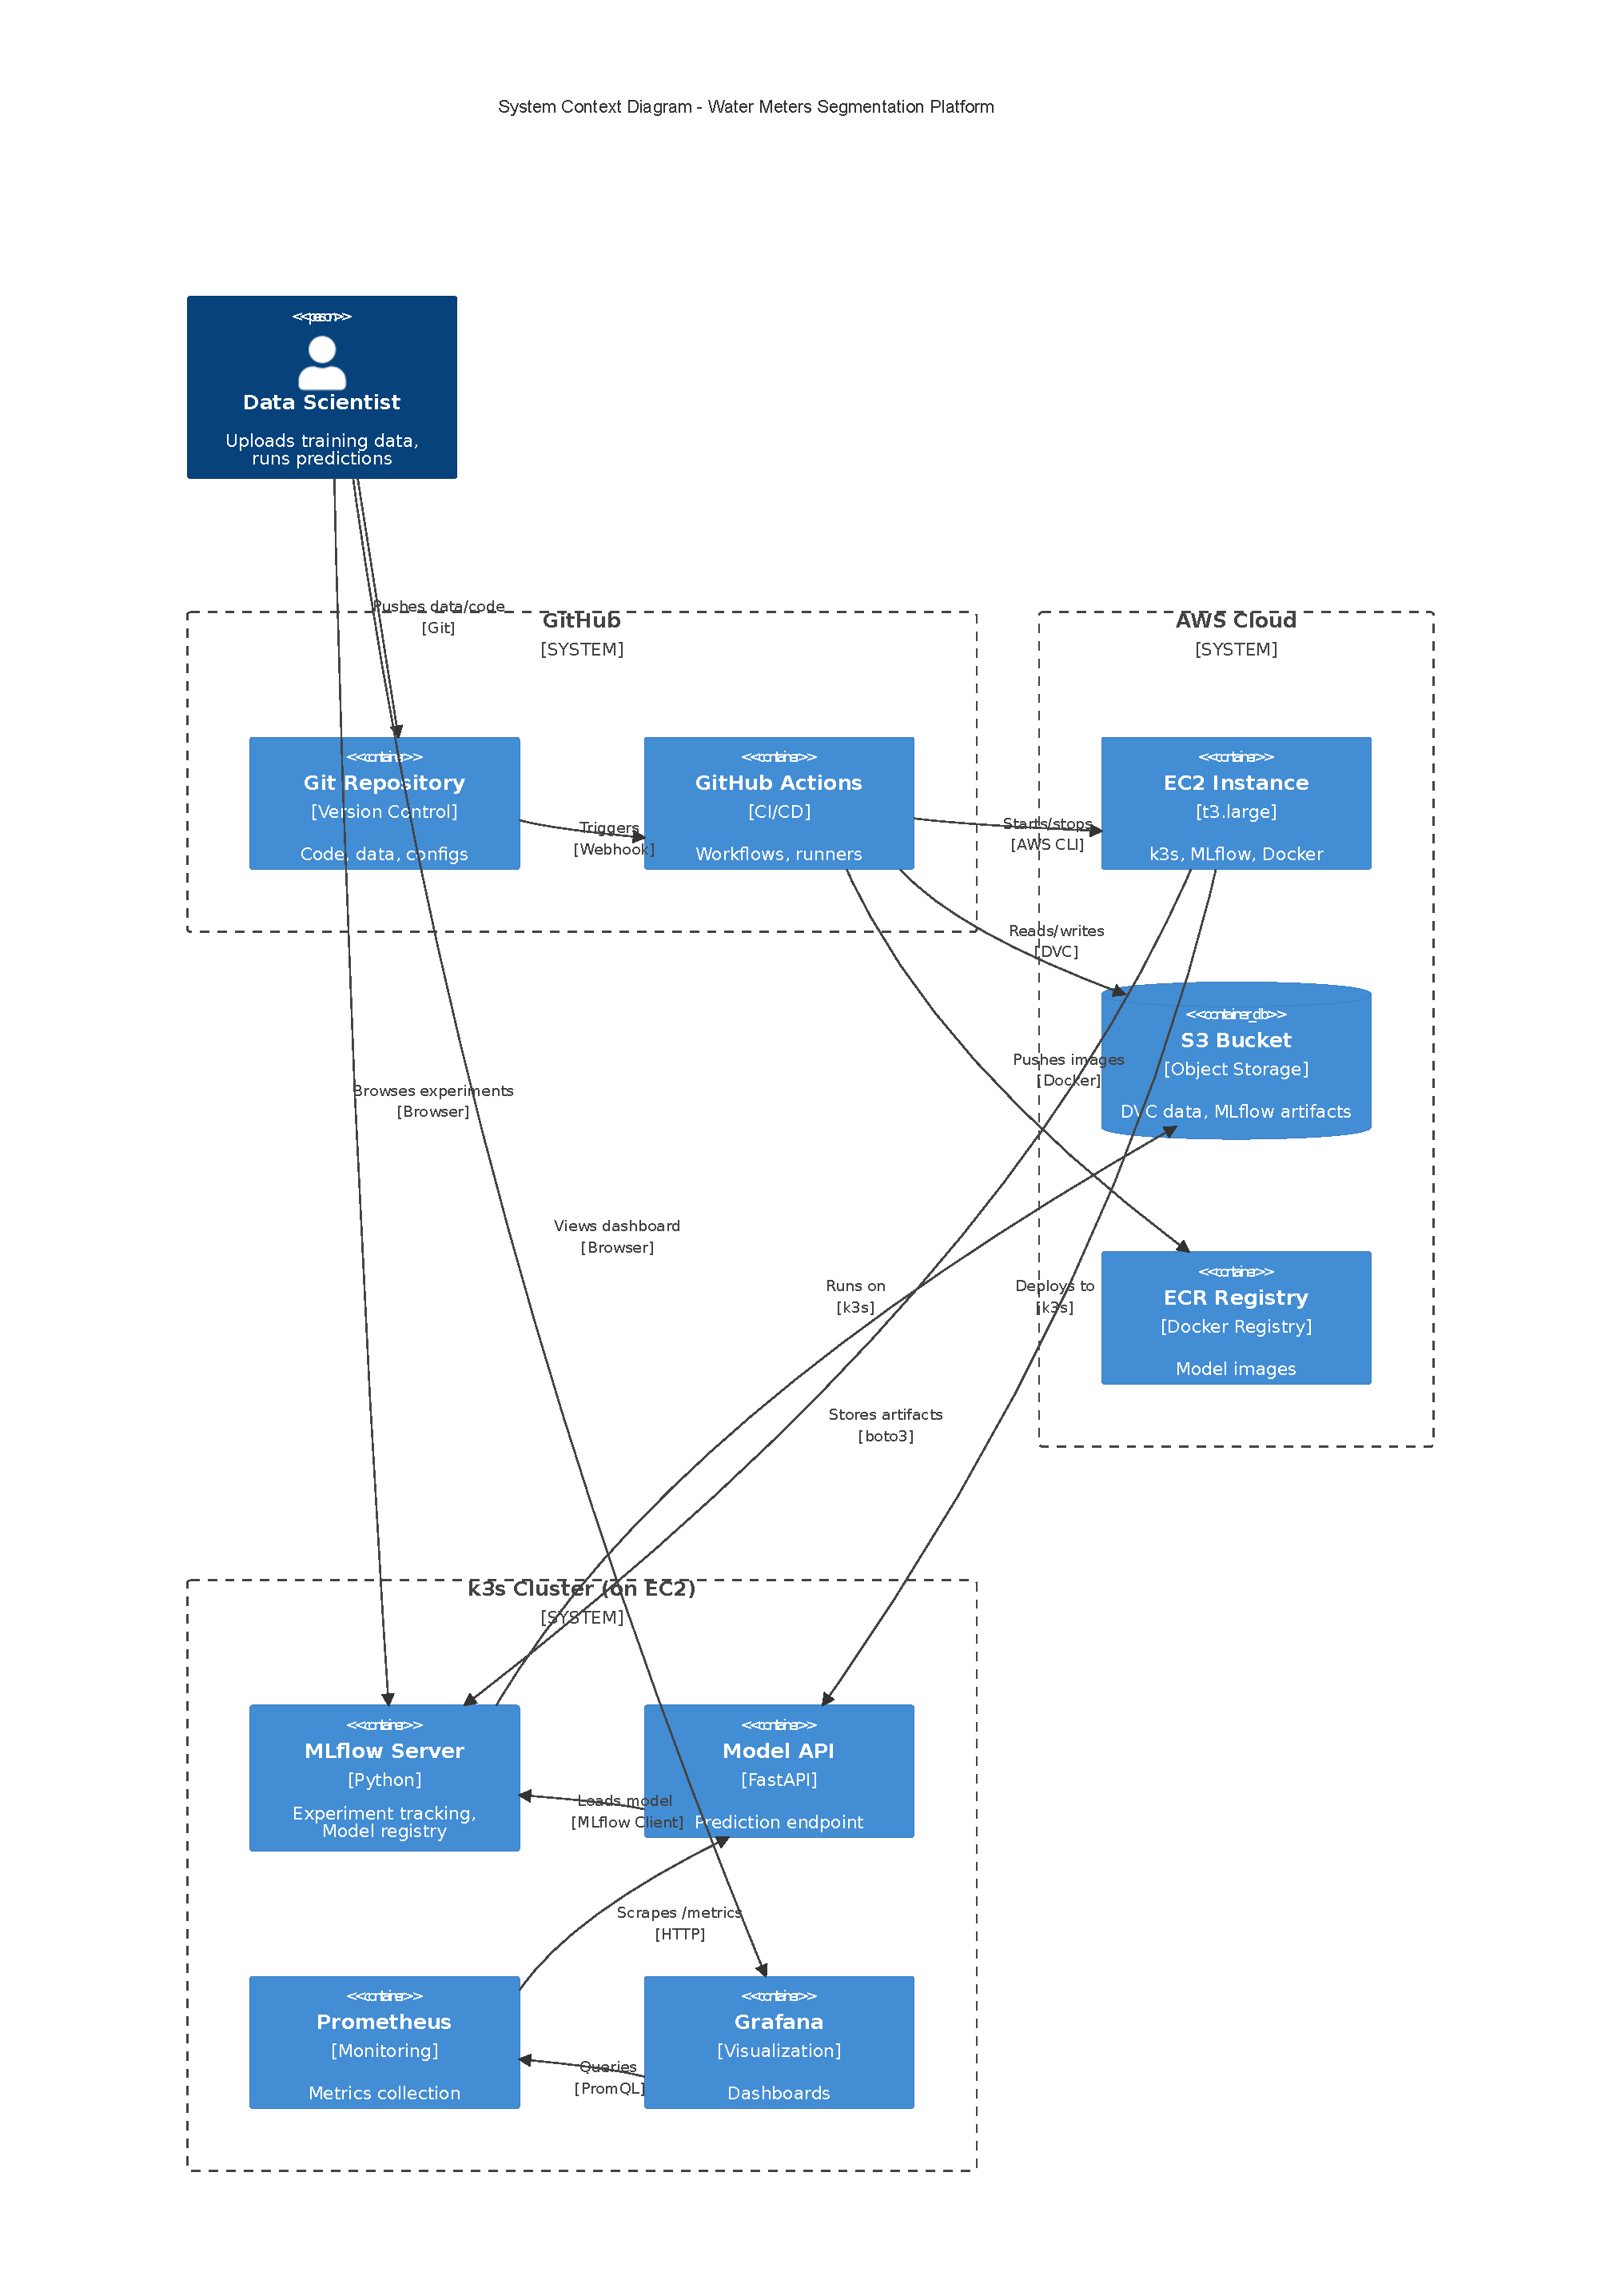
\includegraphics[width=\textwidth]{img/03_architektura_systemu/C4.pdf}%
}{%
  \fbox{\parbox{0.9\textwidth}{\centering\vspace{1.5cm}%
    \textit{[Diagram C4: główne komponenty systemu i ich interakcje]}%
  \vspace{1.5cm}}}%
}
\caption{Architektura systemu --- cztery warstwy i ich komponenty}
\label{fig:architecture-overview}
\end{figure}

% TODO: Diagram C4 wstawić jako C4.pdf (lub C4.png) do img/03_architektura_systemu/
% Diagram powinien pokazywać 4 warstwy (bloki poziome lub pionowe):
%   1. Kontrola wersji: Git/GitHub, DVC -> S3 (dane), Terraform/Helm (IaC)
%   2. Automatyzacja: GitHub Actions (workflow), hook pre-push
%   3. Infrastruktura AWS: EC2 (Elastic IP), S3 (DVC + MLflow), ECR
%   4. Aplikacja: k3s, MLflow Server, API modelu (FastAPI), Prometheus+Grafana
% Ze strzałkami między warstwami: git push -> Actions -> EC2 -> S3/ECR -> k3s

\subsubsection{Warstwa kontroli wersji}

Git i GitHub są centralnym punktem całego systemu --- każda zmiana, czy to w kodzie, danych czy infrastrukturze, przechodzi przez repozytorium. Repozytorium przechowuje kod ML, definicje pipeline'u i infrastruktury, natomiast same pliki binarne danych treningowych przechowywane są w S3 i śledzone przez DVC. Mechanizm \texttt{pre-push hook} automatycznie kieruje nowe dane treningowe na oddzielną gałąź, inicjując cały dalszy proces. Szczegóły działania hooka opisano w rozdziale~\ref{sec:Pipeline_CICD}.

\subsubsection{Warstwa automatyzacji}

GitHub Actions orkiestruje cały cykl życia modelu. Reaguje na pojawienie się nowej gałęzi danych i sekwencyjnie wywołuje: walidację danych, start infrastruktury, trening, bramkę jakości, wdrożenie (jeśli model poprawił się) oraz sprzątanie. Workflow korzysta z reużywalnych składników dla operacji na EC2, co eliminuje powielanie konfiguracji. Szczegółowy opis pipeline'u zawarty jest w rozdziale~\ref{sec:Pipeline_CICD}.

\subsubsection{Warstwa infrastruktury chmurowej}

Cała infrastruktura AWS zdefiniowana jest jako kod w Terraform i tworzona powtarzalnie jednym poleceniem. Kluczowe zasoby to: instancja EC2 ze statycznym Elastic IP (niezbędnym przy cyklicznym stop/start), dwa zasobniki S3 (dane DVC i artefakty MLflow) oraz rejestr obrazów ECR. Instancja EC2 pełni podwójną rolę --- runner treningu podczas pipeline'u i węzeł klastra k3s podczas serwowania modelu. Konfigurację infrastruktury opisuje rozdział~\ref{sec:Wdrozenie_systemu}.

\subsubsection{Warstwa aplikacji i monitoringu}

Na instancji EC2 działa klaster k3s z wdrożonym API modelu (FastAPI, zarządzany przez Helm), serwerem MLflow (systemd) oraz opcjonalnym stosem monitoringu Prometheus~+~Grafana. Model pobierany jest z rejestru MLflow przy starcie kontenera, co oddziela obraz Docker od konkretnej wersji modelu. Szczegóły konfiguracji wdrożenia opisuje rozdział~\ref{sec:Wdrozenie_systemu}.

\subsection{Kluczowe decyzje projektowe}

Tabela~\ref{tab:decisions} zestawia najważniejsze decyzje projektowe podjęte podczas budowy systemu, wraz z uzasadnieniem wyboru i odrzuconą alternatywą. Każda z nich wynika z jednego lub więcej celów wymienionych w sekcji~\ref{sec:Architektura_systemu}.

\begin{table}[H]
\centering
\caption{Kluczowe decyzje architektoniczne}
\label{tab:decisions}
\begin{tabular}{p{3.5cm}p{3.8cm}p{4.2cm}}
\toprule
\textbf{Decyzja} & \textbf{Wybór} & \textbf{Uzasadnienie} \\
\midrule
Orchestracja kontenerów
  & k3s na EC2
  & EKS jest ~15$\times$ droższy; k3s wystarcza dla jednego węzła \\
\addlinespace
Backend MLflow
  & SQLite
  & RDS ~\$30/mies.; SQLite jest wystarczający dla małego projektu; dane Meta przechowywane na EC2 \\
\addlinespace
Dostęp do API
  & NodePort 30080
  & Load Balancer ~\$18/mies.; publiczny adres IP EC2 z Elastic IP jest wystarczający \\
\addlinespace
Tytuł instancji EC2
  & t3.large (8~GB RAM)
  & t3.small/medium: crash OOM przy pobieraniu obrazu PyTorch 8,69~GB; t3.large jest minimum \\
\addlinespace
Stop/start EC2
  & Automatyczny po każdym pipeline
  & EC2 działa tylko ~3--4~h na uruchomienie; oszczędność ~80\% kosztów vs. ciągłe działanie \\
\addlinespace
Dane treningowe w Git
  & Tylko metadane DVC
  & Duże pliki binarne spowalniają Git i przekraczają limity; S3 jest tańszy i skalowalny \\
\addlinespace
Trening przed PR
  & Trening $\rightarrow$ PR (jeśli lepszy)
  & PR tworzony przez bota nie wyzwala innych workflow (ograniczenie GitHub); kolejność eliminuje problem \\
\addlinespace
Baseline bramki jakości
  & Dynamiczny z MLflow
  & Hardkodowany baseline staje się nieaktualny po każdym treningu; MLflow zawsze zna aktualny Production \\
\addlinespace
IAM dla GitHub Actions
  & Tymczasowe klucze sesji
  & AWS Academy zabrania tworzenia ról IAM; OIDC niedostępne; klucze rotowane ręcznie \\
\bottomrule
\end{tabular}
\end{table}

\section{Model Sztucznej Inteligencji}
\label{sec:model_ai}

\subsection{Charakterystyka problemu segmentacji semantycznej}

Model sztucznej inteligencji stanowiący podstawę niniejszego projektu został zaprojektowany do rozwiązywania zadania \textbf{segmentacji semantycznej obrazów wodomierzy}. Celem segmentacji jest przypisanie każdemu pikselowi obrazu etykiety określającej jego przynależność do jednej z wyróżnionych klas, w szczególności obszaru licznika, tarczy oraz tła.

Problem ten ma istotne znaczenie praktyczne w kontekście automatyzacji odczytu wskazań wodomierzy, gdzie poprawne wydzielenie obszaru licznika stanowi warunek konieczny dla dalszych etapów przetwarzania obrazu, takich jak rozpoznawanie cyfr lub analiza wskazań mechanicznych. W przeciwieństwie do klasycznej klasyfikacji obrazów, segmentacja semantyczna wymaga zachowania informacji przestrzennej oraz precyzyjnego odwzorowania granic obiektów, co znacząco zwiększa złożoność problemu.

Dodatkowym wyzwaniem są zmienne warunki akwizycji danych, obejmujące różnice w oświetleniu, kącie wykonania zdjęcia, jakości obrazu oraz stopniu zabrudzenia lub zużycia urządzeń pomiarowych. Czynniki te powodują, że klasyczne algorytmy przetwarzania obrazu okazują się niewystarczające, co uzasadnia zastosowanie metod opartych na uczeniu głębokim.

\begin{figure}[H]
  \centering
  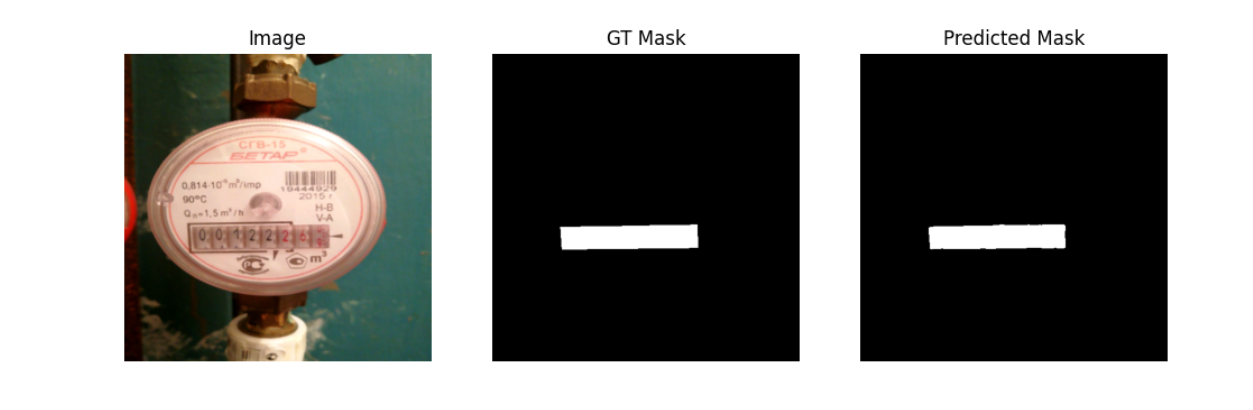
\includegraphics[width=\textwidth]{img/04_model_sztucznej_inteligencji/Example_Prediction.png}
  \caption{Przykład predykcji modelu segmentacji semantycznej}
  \label{fig:example_prediction}
\end{figure}

\subsection{Architektura modelu}

W projekcie wykorzystano konwolucyjną sieć neuronową opartą na architekturze \textbf{U-Net}, powszechnie stosowaną w zadaniach segmentacji semantycznej obrazów. Architektura ta charakteryzuje się symetryczną budową typu encoder--decoder, umożliwiającą jednoczesne wydobywanie cech semantycznych oraz zachowanie informacji przestrzennej.

Część kodująca (encoder) odpowiada za stopniowe przekształcanie obrazu wejściowego do reprezentacji o coraz wyższym poziomie abstrakcji poprzez sekwencję operacji konwolucji oraz redukcji rozdzielczości. Część dekodująca (decoder) realizuje proces rekonstrukcji obrazu wyjściowego, przywracając jego pierwotną rozdzielczość i generując maskę segmentacyjną.

Kluczowym elementem architektury są tzw. \textit{skip connections}, umożliwiające bezpośrednie przekazywanie map cech pomiędzy odpowiadającymi sobie poziomami enkodera i dekodera. Mechanizm ten pozwala ograniczyć utratę informacji lokalnej oraz poprawić jakość segmentacji, szczególnie w obszarach granicznych pomiędzy klasami.

Zastosowana implementacja architektury U-Net została dostosowana do specyfiki problemu, w tym rozdzielczości obrazów wejściowych oraz liczby klas segmentacyjnych. Model generuje maskę wyjściową o tej samej rozdzielczości co obraz wejściowy, co ułatwia dalsze etapy przetwarzania oraz ocenę jakości predykcji.

\begin{figure}[H]
  \centering
  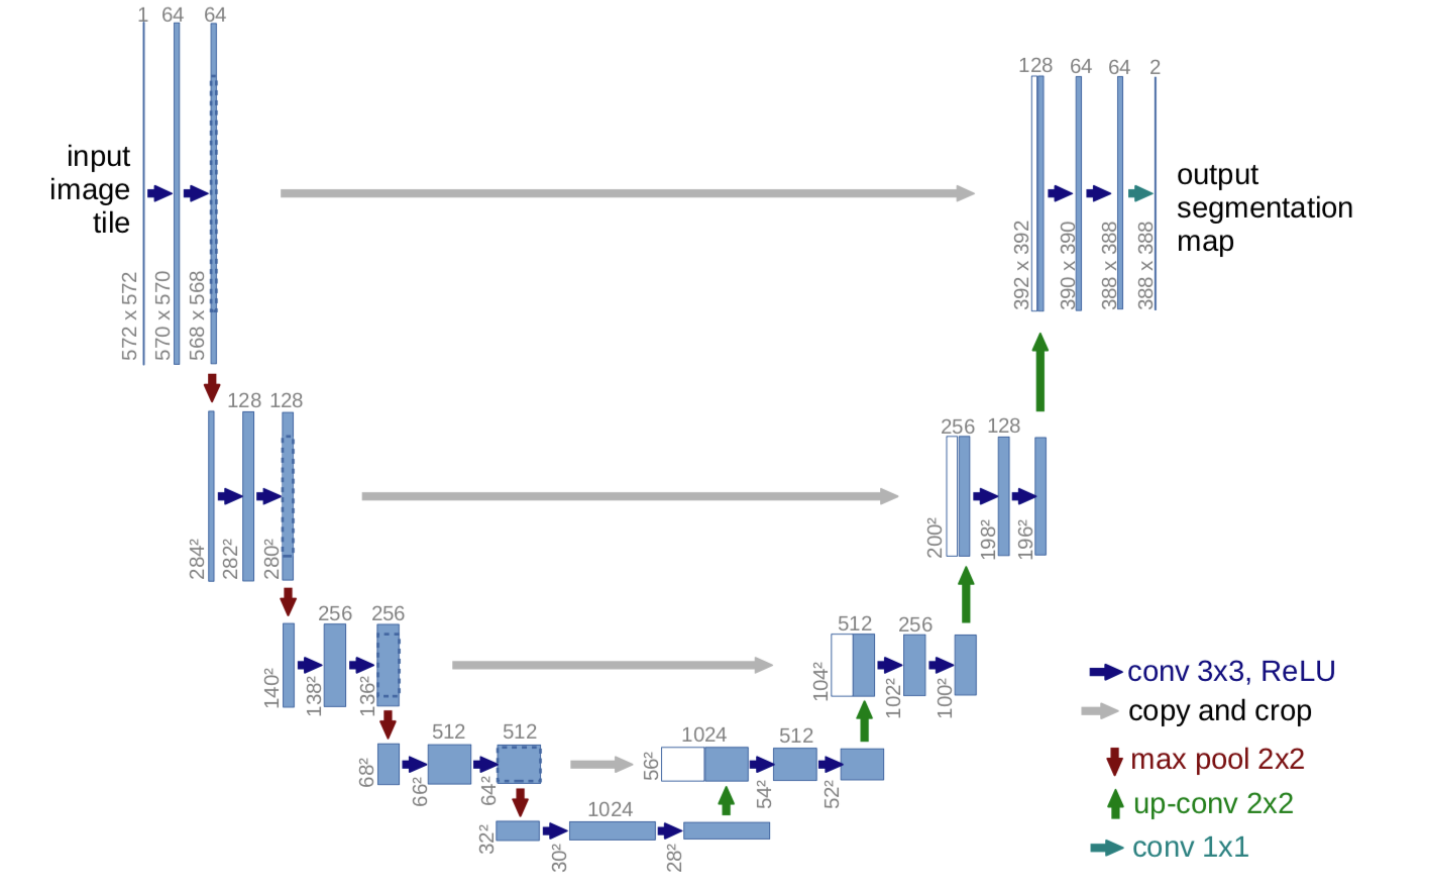
\includegraphics[width=\textwidth]{img/04_model_sztucznej_inteligencji/U-NET.png}
  \caption{Schemat architektury U-Net \cite{unet_segmentacja_blog}}
  \label{fig:unet_architecture}
\end{figure}

\subsection{Dane treningowe i przygotowanie zbioru danych}

Model został wytrenowany na zbiorze danych składającym się z obrazów wodomierzy oraz odpowiadających im masek. Każda próbka zawiera obraz wejściowy w postaci fotografii oraz maskę określającą przynależność poszczególnych pikseli do zdefiniowanych klas.

Proces przygotowania danych obejmował normalizację wartości pikseli, standaryzację rozdzielczości obrazów oraz podział zbioru danych na część treningową, walidacyjną i testową. W celu zwiększenia odporności modelu na zmienność danych wejściowych zastosowano techniki augmentacji danych, takie jak losowe obroty, skalowanie, przesunięcia oraz modyfikacje jasności i kontrastu.

Zastosowanie augmentacji pozwala ograniczyć ryzyko przeuczenia modelu oraz poprawić jego zdolność do generalizacji na dane niewidziane w procesie uczenia. Istotnym aspektem projektu jest fakt, że zbiór danych oraz jego kolejne wersje podlegają wersjonowaniu, co umożliwia jednoznaczne powiązanie konkretnej wersji modelu z użytymi danymi treningowymi.

Zbiór danych wykorzystany w projekcie pochodzi z platformy Kaggle \cite{kaggle_water_meters}.

\subsection{Proces uczenia i metryki jakości}

Proces uczenia modelu realizowany jest w sposób nadzorowany, z wykorzystaniem funkcji straty dostosowanej do problemu segmentacji semantycznej. Jako główne metryki oceny jakości modelu zastosowano \textbf{współczynnik Dice} oraz \textbf{Intersection over Union (IoU)}, które są standardowymi miarami stosowanymi w zadaniach segmentacyjnych.

Współczynnik Dice umożliwia ocenę stopnia pokrycia obszaru przewidywanego przez model z obszarem referencyjnym, natomiast IoU mierzy stosunek części wspólnej obu obszarów do ich sumy. Zastosowanie obu metryk pozwala na bardziej kompleksową ocenę jakości predykcji, szczególnie w przypadku niezbalansowanych klas.

Proces uczenia realizowany jest iteracyjnie, z wykorzystaniem zbioru walidacyjnego do monitorowania jakości modelu oraz ograniczania zjawiska przeuczenia. Najlepsza wersja modelu, zgodnie z przyjętymi kryteriami jakości, zapisywana jest jako artefakt i przekazywana do dalszych etapów zautomatyzowanego pipeline’u CI/CD.

\subsection{Model jako artefakt w procesie CI/CD}

W kontekście niniejszej pracy model sztucznej inteligencji traktowany jest jako pełnoprawny artefakt inżynierski, podlegający wersjonowaniu, testowaniu oraz kontrolowanemu wdrażaniu. Każda wersja modelu jest jednoznacznie powiązana z wersją kodu źródłowego, zestawem danych treningowych, konfiguracją hiperparametrów oraz uzyskanymi metrykami jakości.

Takie podejście umożliwia pełną reprodukowalność wyników oraz stanowi podstawę do dalszej analizy porównawczej pomiędzy podejściem manualnym a zautomatyzowanym procesem CI/CD. Szczegółowa analiza wpływu automatyzacji na jakość, stabilność oraz koszty utrzymania modeli sztucznej inteligencji zostanie przedstawiona w kolejnych rozdziałach pracy.

\begin{figure}[H]
  \centering
  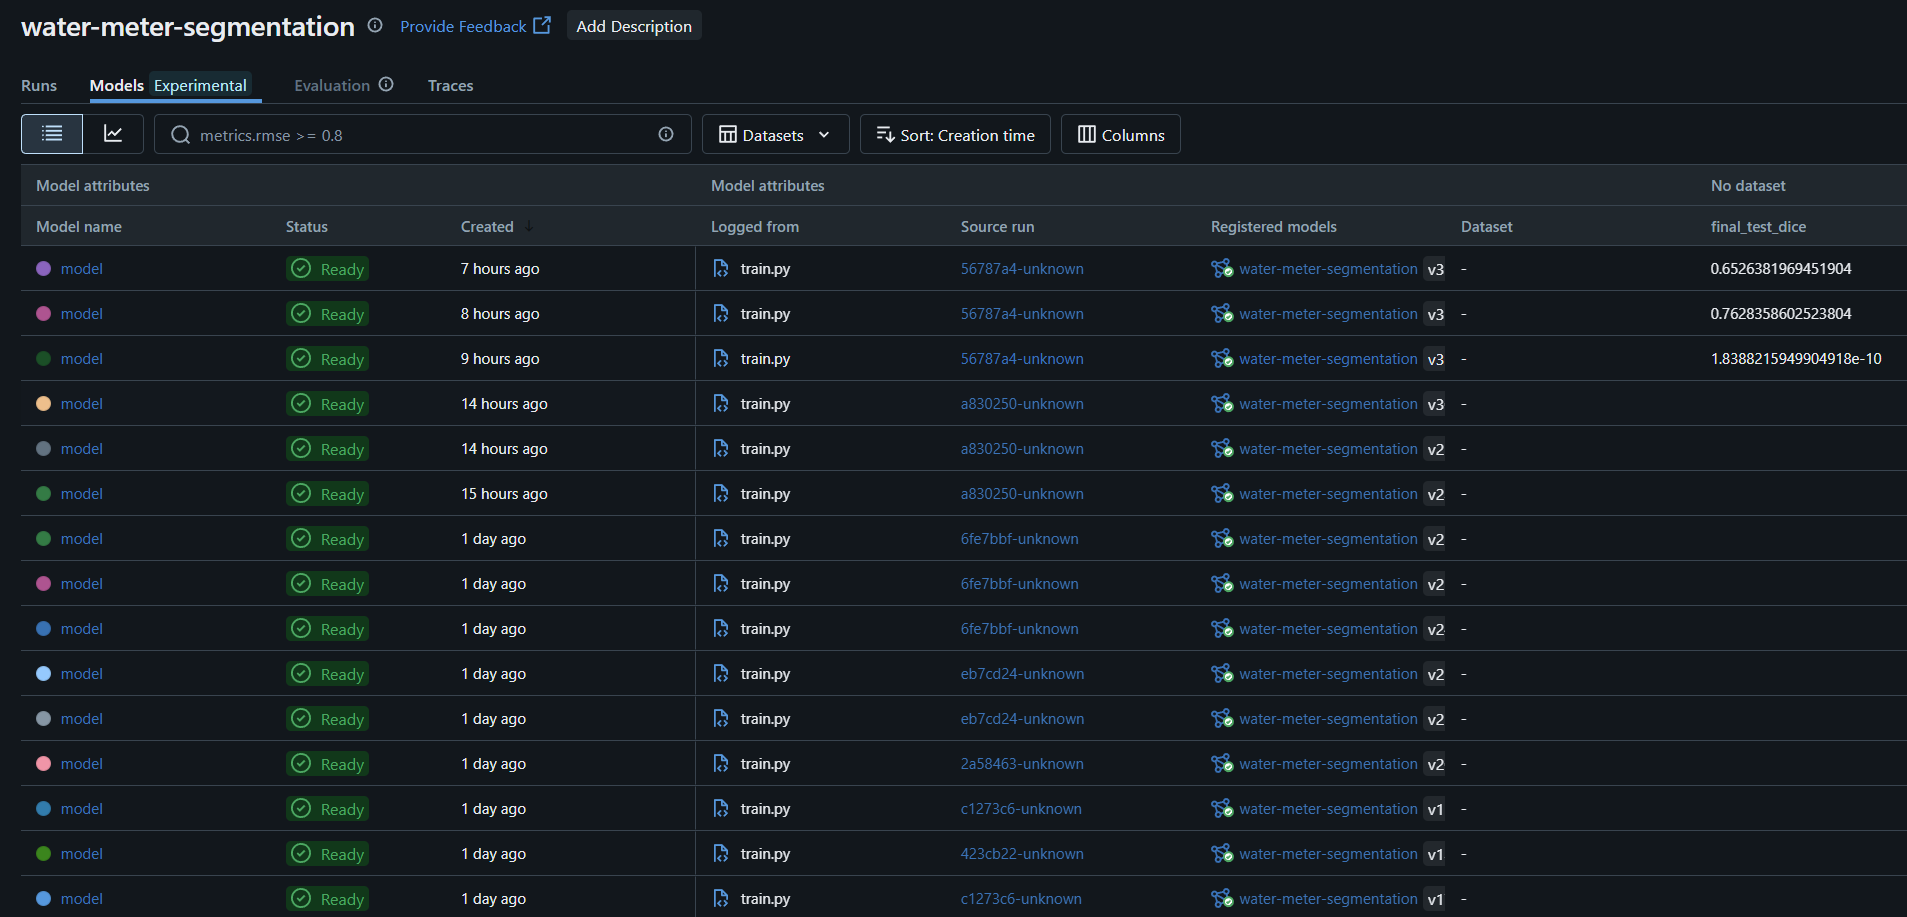
\includegraphics[width=\textwidth]{img/04_model_sztucznej_inteligencji/mlflow_versions.png}
  \caption{Wersjonowanie modeli w rejestrze MLflow}
  \label{fig:mlflow_versions}
\end{figure}

\section{Pipeline CI/CD}
\label{sec:Pipeline_CICD}

Rozdział opisuje implementację zautomatyzowanego pipeline CI/CD dla modeli uczenia maszynowego. Prezentowane rozwiązanie realizuje przepływ: dodanie danych treningowych przez użytkownika wyzwala sekwencję kroków --- walidację, trening, ocenę jakości i wdrożenie --- bez konieczności ręcznej interwencji.

\subsection{Hook pre-push}

Pierwszym elementem pipeline jest hook Git \texttt{pre-push} \cite{chacon2014pro_git}, instalowany lokalnie na maszynie użytkownika przez skrypt \texttt{devops/scripts/install-git-hooks.sh}. Hook uruchamia się automatycznie przed każdym \texttt{git push} i sprawdza, czy w zestawie zmian znajdują się pliki w katalogach \texttt{WMS/data/training/images/} lub \texttt{WMS/data/training/masks/}.

Jeśli zmiany dotyczą danych treningowych, hook:
\begin{enumerate}
  \item tworzy nową gałąź o nazwie \texttt{data/TIMESTAMP} (np. \texttt{data/20260215-143022}),
  \item commituje do niej wyłącznie nowe pliki z katalogów danych,
  \item przekierowuje push na tę gałąź zamiast na \texttt{main}.
\end{enumerate}

Całość wykonuje się w mniej niż 10 sekund, ponieważ hook nie wymaga połączenia z AWS ani lokalnych poświadczeń chmurowych. Merge danych z historycznym zbiorem w S3 odbywa się po stronie GitHub Actions.

\begin{figure}[H]
  \centering
  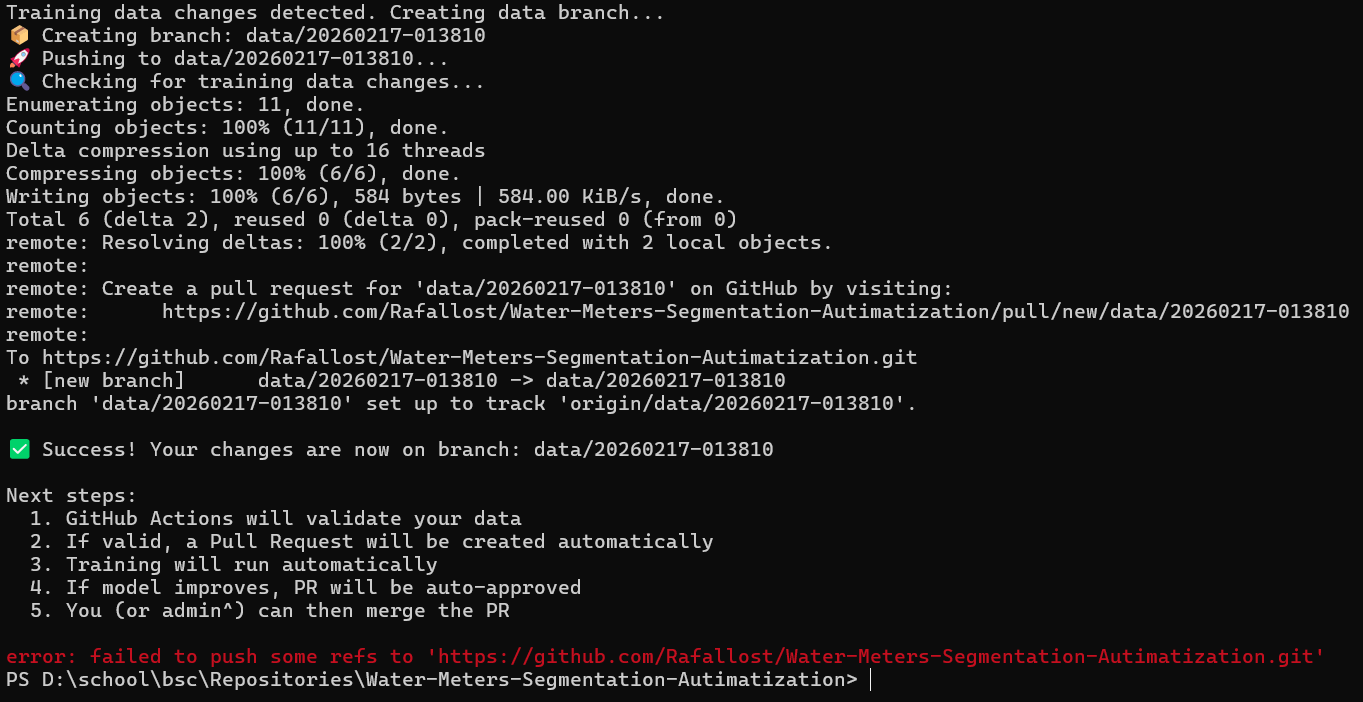
\includegraphics[width=\linewidth]{img/05_pipline_ci_cd/hook.png}
  \caption{Wynik wypchania nowych danych na gałąź \texttt{data/TIMESTAMP}.}
\end{figure}

\subsection{Walidacja danych}

\begin{sloppypar}
Po wypchnięciu gałęzi danych uruchamia się pierwszy job workflow \texttt{training-data-pipeline.yaml} \cite{github_actions_docs}: \texttt{merge-and-validate}. Składa się on z dwóch faz.
\end{sloppypar}

\paragraph{Faza scalania}\mbox{}\\
Job pobiera istniejące dane z Amazon S3 (za pomocą poświadczeń przechowywanych w sekretach GitHub), scala je z nowo dostarczonymi plikami i aktualizuje manifesty DVC. Scalanie jest idempotentne --- pliki o identycznej nazwie i sumie kontrolnej nie są duplikowane.

\paragraph{Faza walidacji}\mbox{}\\
Skrypt \texttt{validate\_data.py} weryfikuje scalony zbiór danych pod kątem czterech kryteriów:
\begin{itemize}
  \item \textbf{kompletność par} --- dla każdego obrazu w katalogu \texttt{images/} musi istnieć maska o tej samej nazwie w \texttt{masks/} (porównanie po \textit{stem} nazwy pliku),
  \item \textbf{rozdzielczość} --- każdy plik obrazu i maski musi mieć rozdzielczość dokładnie $512 \times 512$ px,
  \item \textbf{binarność masek} --- maski mogą zawierać wyłącznie wartości $0$ i $255$ (brak półprzezroczystości),
  \item \textbf{format pliku} --- akceptowane są formaty \texttt{.jpg} oraz \texttt{.png}.
\end{itemize}

Wynik walidacji jest publikowany jako komentarz w pull requeście. W przypadku błędów komentarz zawiera listę plików niezgodnych z wymaganiami, a dalsze jobe są pomijane (warunkowanie przez \texttt{needs} i \texttt{if: needs.merge-and-validate.outputs.valid == 'true'}).

\begin{verbatim}
# Fragment skryptu walidacji
for img_stem in image_stems:
    if img_stem not in mask_stems:
        errors.append(f"Brak maski dla: {img_stem}")
\end{verbatim}

\begin{figure}[H]
    \centering
    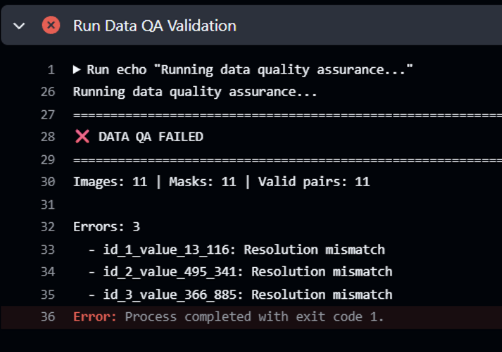
\includegraphics[width=0.7\linewidth]{img/05_pipline_ci_cd/example_qa_stop.png}
    \caption{Przykład komentarza z wynikiem walidacji danych. W tym przypadku wykryto złą rozdzielczość, co skutkuje zatrzymaniem dalszych kroków pipeline.}
    \label{fig:workflow-concurrency}
\end{figure}

\subsection{Pipeline treningowy}

Główny workflow \texttt{training-data-pipeline.yaml} składa się z ośmiu jobów. Joby 1--3 wykonywane są sekwencyjnie. Po zakończeniu treningu workflow rozgałęzia się: gdy model się nie poprawił, uruchamia się \texttt{stop-infra} (job 4); gdy model się poprawił --- równolegle uruchamiają się \texttt{deploy} (job 5) i \texttt{create-pr} (job 7). Job 6 zatrzymuje EC2 po wdrożeniu, a job 8 finalizuje scalenie.

\begin{figure}[H]
    \centering
    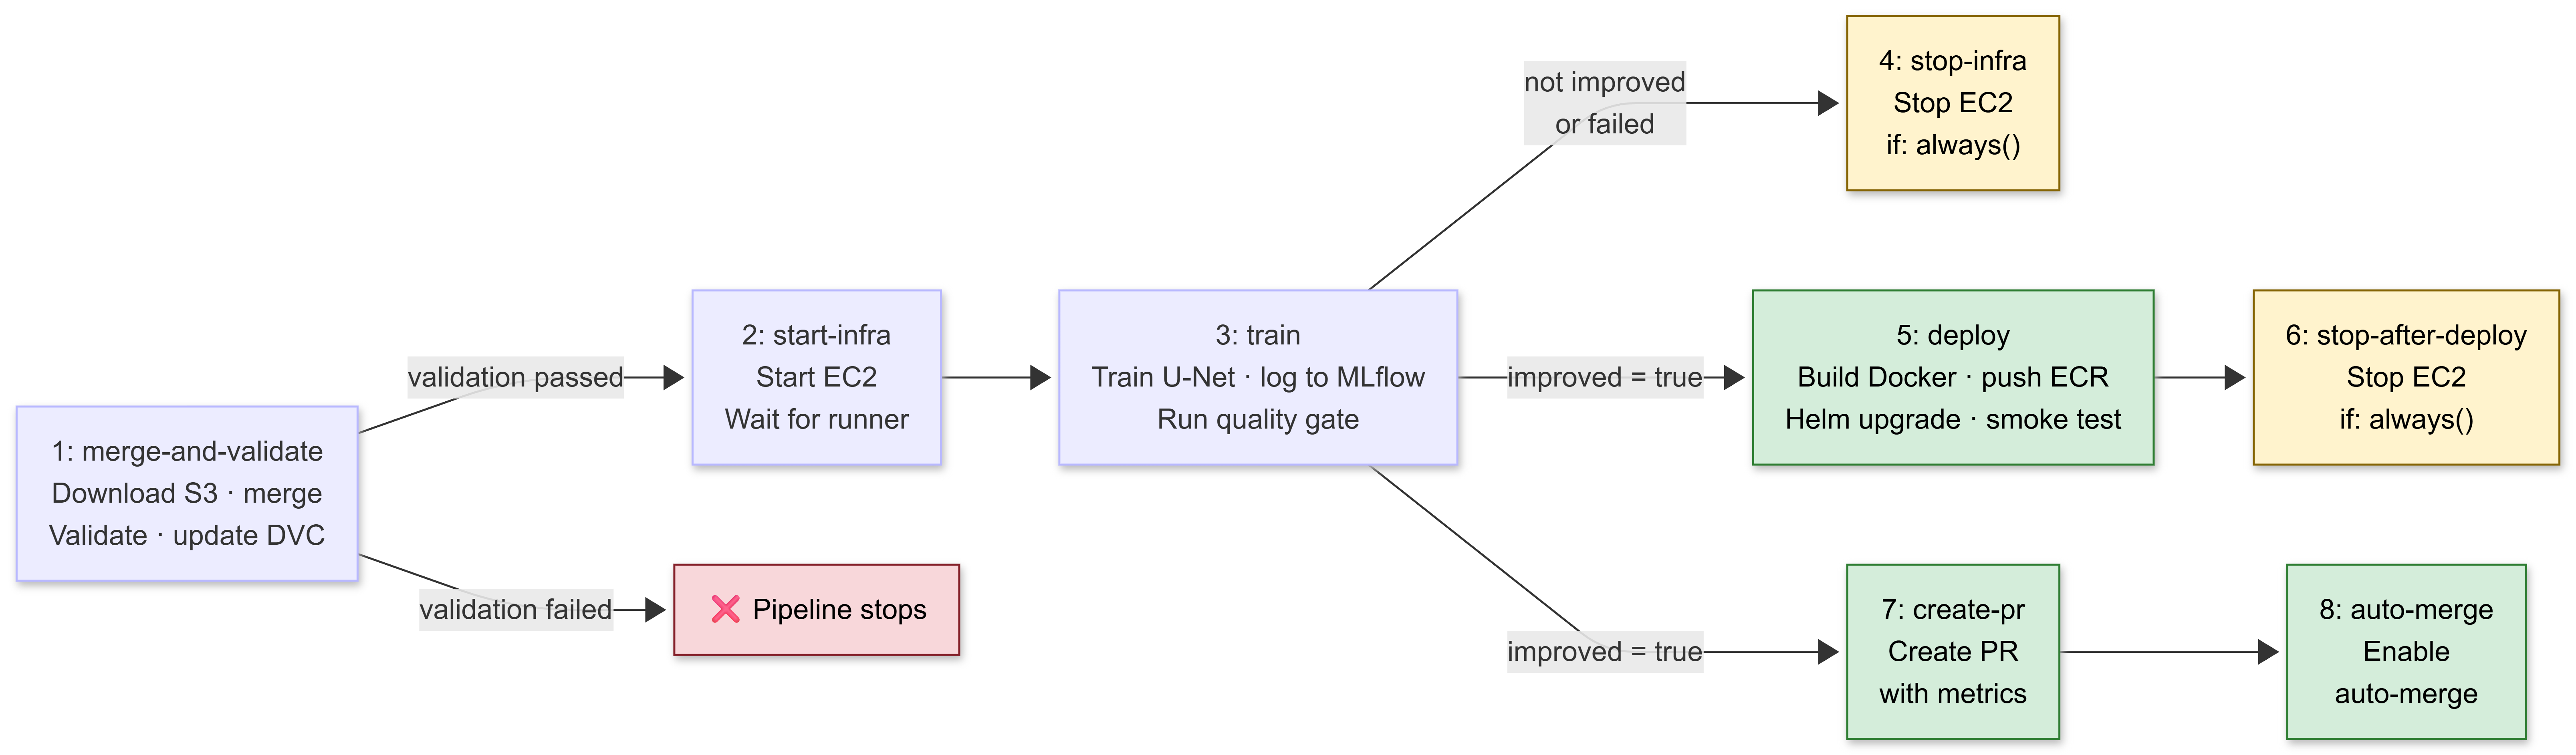
\includegraphics[width=\linewidth]{img/05_pipline_ci_cd/Training_pipline.png}
    \caption{Sekwencja jobów w workflow \texttt{training-data-pipeline.yaml}}
    \label{fig:workflow-jobs}
\end{figure}

\paragraph{Job 1: merge-and-validate}\mbox{}\\
Opracowane we wcześniejszym fragmencie. Pobiera istniejące dane z S3, scala je z nowo dostarczonymi plikami, uruchamia walidację, aktualizuje manifesty DVC i przesyła scalony zbiór jako artefakt GitHub Actions..

\paragraph{Job 2: start-infra}\mbox{}\\
Wykonuje się na hoście GitHub (nie na EC2) i jest odpowiedzialny wyłącznie za uruchomienie infrastruktury. Wywołuje AWS CLI (\texttt{aws ec2 start-instances}) z identyfikatorem instancji zapisanym w sekretach repozytorium. Po wysłaniu polecenia co 30 sekund sprawdza API GitHub, czy self-hosted runner przypisany do tej instancji pojawił się w stanie \textit{online} --- czeka maksymalnie 10 minut. Dzięki temu każdy kolejny job pewnie trafi na już działającą instancję.

\paragraph{Job 3: train}\mbox{}\\
Jedyny job wykonywany na self-hosted runnerze, czyli bezpośrednio na instancji EC2. Pobiera scalony zbiór danych z artefaktu GitHub Actions, uruchamia skrypt \texttt{train.py}, który inicjalizuje model U-Net z seedem równym numerowi uruchomienia (\texttt{run\_number}), trenuje przez zdefiniowaną liczbę epok i loguje metryki \texttt{val\_dice} oraz \texttt{val\_iou} do MLflow. Po zakończeniu treningu skrypt \texttt{quality\_gate.py} pobiera metryki aktualnego modelu Production z rejestru MLflow, porównuje je z wynikami nowego treningu i ustawia output \texttt{improved=true} lub \texttt{improved=false}, sterując dalszym przebiegiem workflow.

\paragraph{Job 4: stop-infra}\mbox{}\\
Zatrzymuje instancję EC2 gdy trening zakończył się błędem lub model nie poprawił wyników (\texttt{if: always() \&\& (train.result != 'success' || improved != 'true')}). Jest to reużywalny workflow wywołujący \texttt{aws ec2 stop-instances}. Dzięki warunkowi \texttt{always()} job uruchamia się nawet gdy poprzednie jobe zakończyły się wyjątkiem, eliminując ryzyko pozostawienia uruchomionej instancji i nieoczekiwanych kosztów.

\paragraph{Job 5: deploy}\mbox{}\\
Uruchamia się wyłącznie jeśli model spełnił kryteria bramki jakości (\texttt{if: improved == 'true'}). Wykonuje się na self-hosted runnerze na EC2. Buduje obraz Docker na podstawie \texttt{docker/Dockerfile.serve}, taguje go numerem wersji i hashiem commita, uwierzytelnia się w Amazon ECR i wgrywa obraz. Następnie wywołuje \texttt{helm upgrade}, który zaktualizuje deployment na klastrze k3s do nowej wersji obrazu --- kontener przy starcie pobiera model ze stadium Production z rejestru MLflow, co oddziela wersję obrazu od wersji modelu. Po wdrożeniu wykonywany jest smoke test sprawdzający dostępność endpointów \texttt{/health}, \texttt{/predict} i \texttt{/metrics}.

\paragraph{Job 6: stop-after-deploy}\mbox{}\\
Zatrzymuje instancję EC2 po zakończeniu joba \texttt{deploy} (\texttt{if: always()}). Stanowi odpowiednik \texttt{stop-infra} dla ścieżki, gdy model się poprawił. Istnieje jako osobny job, ponieważ \texttt{deploy} korzysta z runnera na EC2 --- instancja musi pozostać uruchomiona do końca wdrożenia i może zostać zatrzymana dopiero po jego zakończeniu.

\paragraph{Job 7: create-pr}\mbox{}\\
Uruchamia się równolegle z jobem \texttt{deploy}, jeśli model spełnił kryteria bramki jakości. Tworzy pull request z gałęzi danych do \texttt{main} z automatycznie generowanym opisem zawierającym zestawienie metryk: wartości \texttt{val\_dice} i \texttt{val\_iou} nowego modelu oraz poprzedniego baseline, a także link do uruchomienia MLflow. Pull request scala zaktualizowane manifesty DVC (\texttt{images.dvc}, \texttt{masks.dvc}) z gałęzią główną, trwale łącząc wersję kodu z wersją danych.

\paragraph{Job 8: auto-merge}\mbox{}\\
Włącza automatyczne scalanie pull requesta przez API GitHub (\texttt{gh pr merge --auto}). Scalenie następuje natychmiast po pozytywnym przejściu statusowych sprawdzeń wymaganych przez reguły ochrony gałęzi. W efekcie, jeśli model się poprawił, cały cykl --- od wypchnięcia danych do scalenia z \texttt{main} --- odbywa się bez żadnej ręcznej interwencji.

\begin{figure}[H]
    \centering
    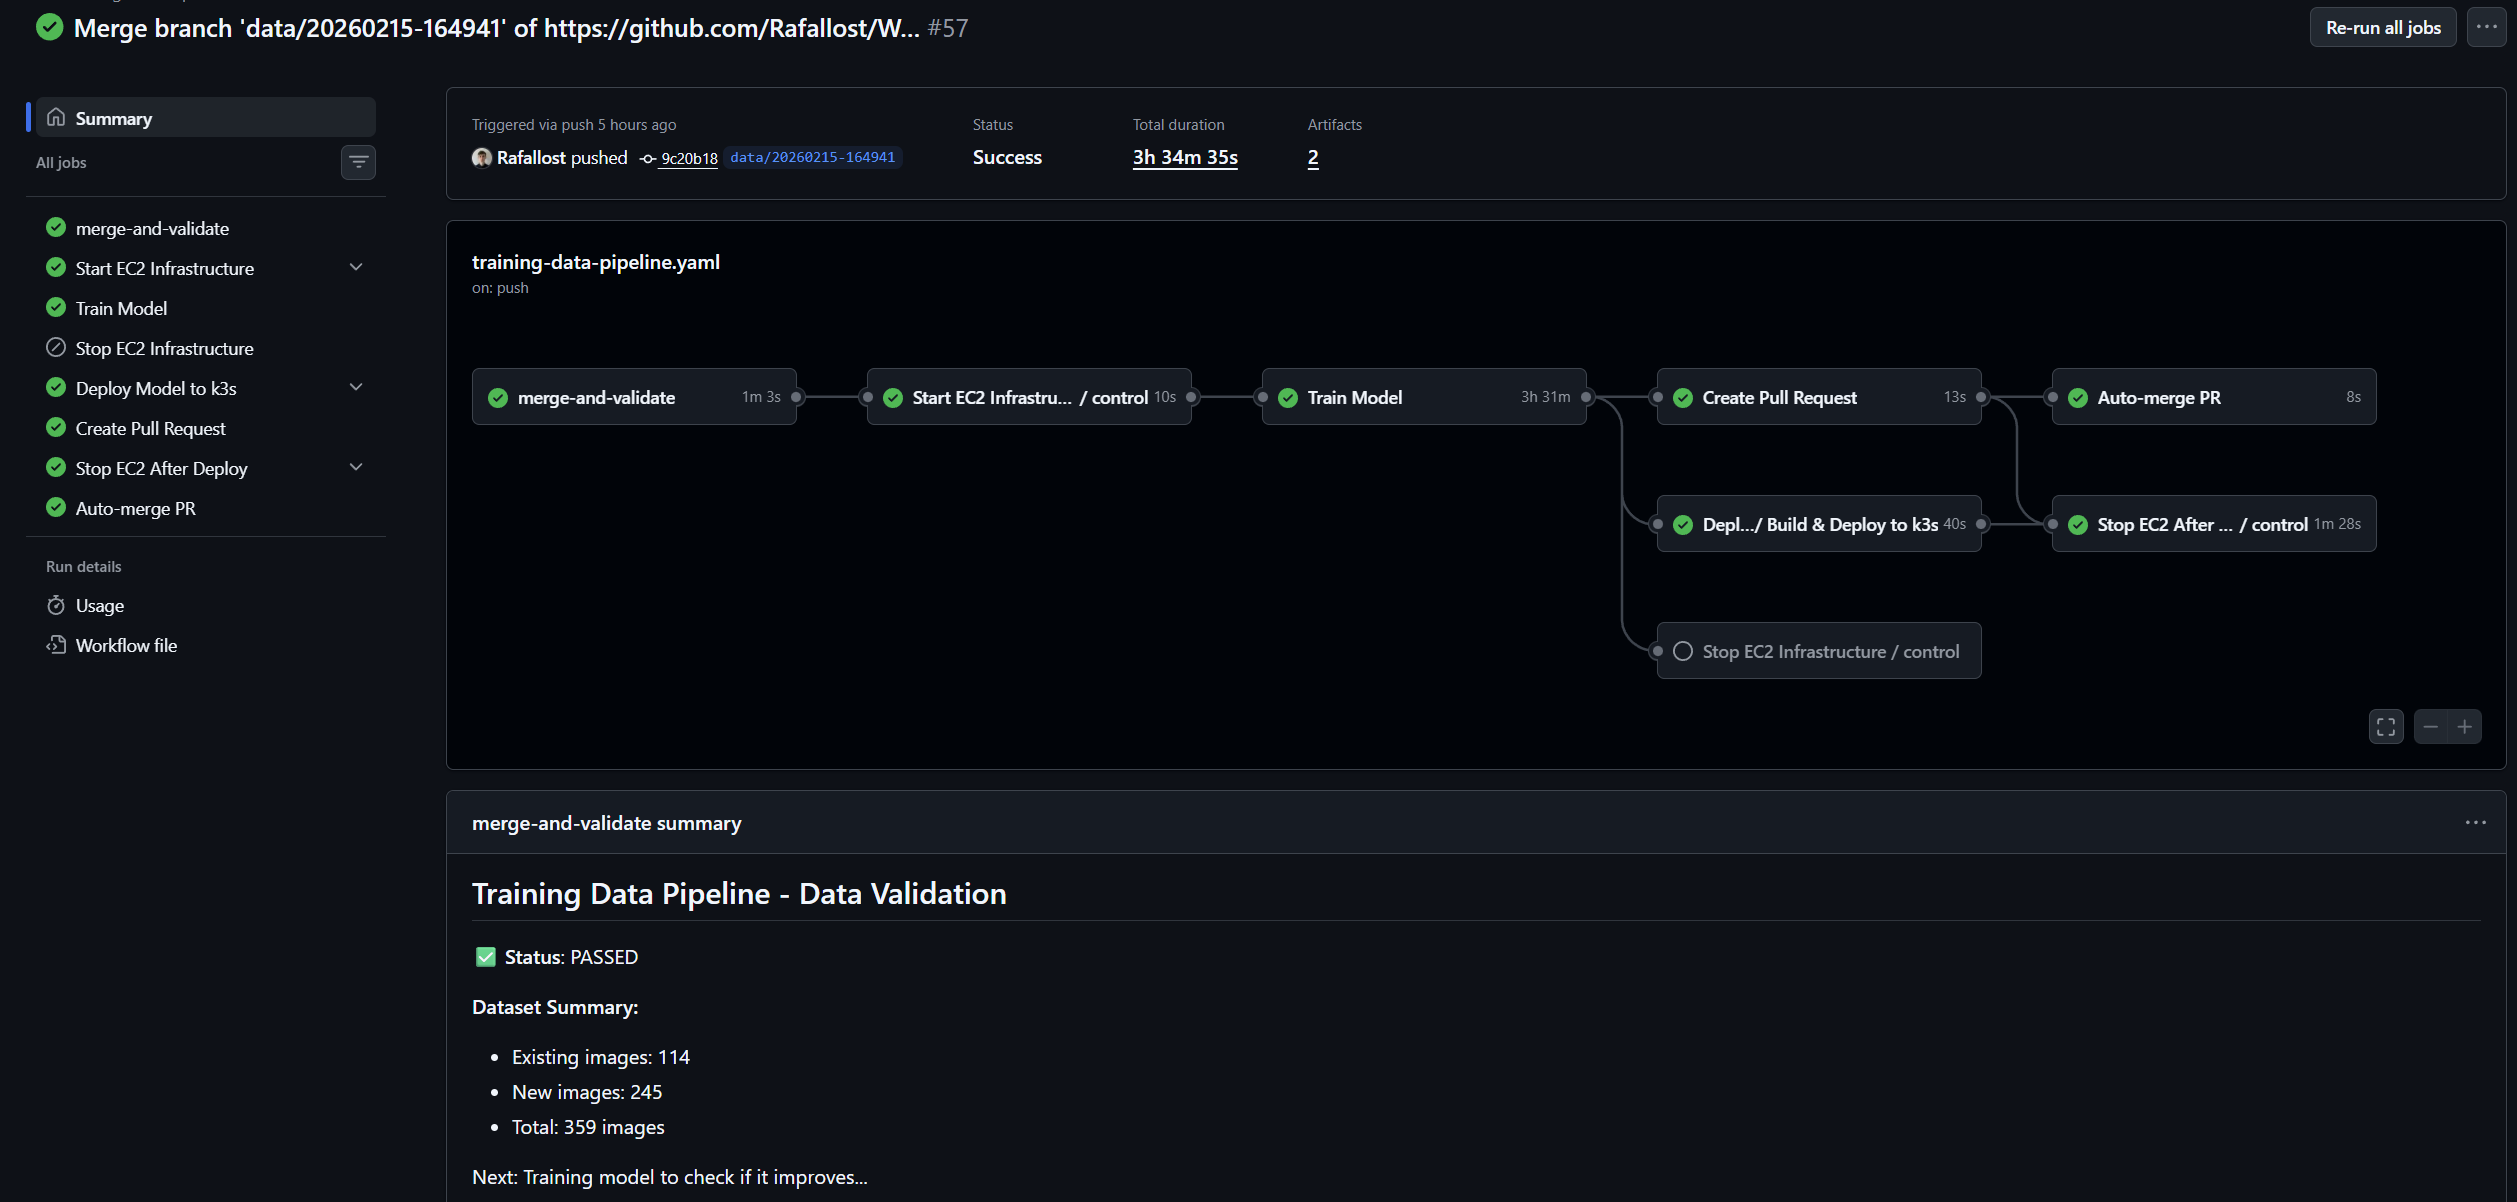
\includegraphics[width=1.0\linewidth]{img/05_pipline_ci_cd/successfull_training.png}
    \caption{Udany przebieg pipeline CI/CD z automatycznym wdrożeniem nowej wersji modelu.}
    \label{fig:workflow-success}
\end{figure}

\subsection{Współbieżność i kolejkowanie}

Workflow skonfigurowany jest z kluczem \texttt{concurrency.cancel-in-progress: false}. Oznacza to, że jeśli użytkownik wypchnął dane kilkakrotnie zanim poprzednie uruchomienie zdążyło się zakończyć, kolejne uruchomienia nie są anulowane --- trafiają do kolejki i wykonują się po zakończeniu poprzednich. Podejście to chroni przed sytuacją, w której późniejszy push nadpisze wyniki wcześniejszego treningu, zanim zostanie on oceniony przez bramkę jakości.

\begin{figure}[H]
    \centering
    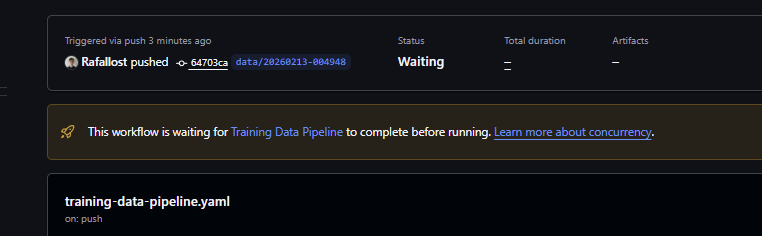
\includegraphics[width=1.0\linewidth]{img/05_pipline_ci_cd/concurrency.png}
    \caption{Kolejkowanie uruchomień workflow w GitHub Actions --- nowe uruchomienie czeka na zakończenie poprzedniego.}
    \label{fig:workflow-concurrency}
\end{figure}

\subsection{Bramka jakości}

Bramka jakości jest mechanizmem decydującym, czy nowy model jest wystarczająco dobry, żeby trafić do produkcji. Implementacja jest w skrypcie \texttt{quality\_gate.py} i korzysta z API MLflow Model Registry \cite{mlflow_model_registry}.

\paragraph{Pobieranie baseline}\mbox{}\\
Skrypt łączy się z MLflow przez \texttt{MlflowClient} i pobiera metryki aktualnego modelu Production:

\begin{verbatim}
client = MlflowClient(tracking_uri=mlflow_uri)
versions = client.get_latest_versions(
    "water-meter-segmentation",
    stages=["Production"]
)
if versions:
    baseline_run = client.get_run(versions[0].run_id)
    baseline_dice = float(
        baseline_run.data.metrics["val_dice"]
    )
else:
    baseline_dice = 0.0  # pierwsze trenowanie
\end{verbatim}

\paragraph{Logika decyzyjna}\mbox{}\\
Model jest uznany za ulepszony, jeśli obie metryki walidacyjne są wyższe od baseline:

\begin{itemize}
  \item \texttt{val\_dice > baseline\_dice}
  \item \texttt{val\_iou > baseline\_iou}
\end{itemize}

Jeśli warunek jest spełniony, skrypt promuje nowy model do etapu Production w MLflow i archiwizuje poprzednią wersję. Wynik jest przekazywany jako output do GitHub Actions (\texttt{echo "improved=true" >> \$GITHUB\_OUTPUT}).

\subsection{Automatyczne wdrożenie}

Gdy bramka jakości potwierdzi poprawę modelu, job \texttt{deploy} w tym samym workflow buduje i wdraża nowy obraz Docker na klastrze k3s --- równolegle z tworzeniem pull requesta (job \texttt{create-pr}).

\paragraph{Budowanie obrazu}\mbox{}\\
Obraz jest budowany na podstawie pliku \texttt{docker/Dockerfile.serve}. Używa warstwy bazowej z PyTorch CPU, kopiuje kod API i instaluje zależności z \texttt{requirements.txt}. Po zbudowaniu obraz jest tagowany numerem wersji i hashiem commita, a następnie wysyłany do Amazon ECR.

\paragraph{Wdrożenie Helm}\mbox{}\\
Helm \cite{helm_docs} aktualizuje deployment na klastrze k3s \cite{k3s_docs} nową wersją obrazu. Konfiguracja wdrożenia zdefiniowana jest w \texttt{infrastructure/helm-values.yaml}. Po wdrożeniu automatycznie wykonywany jest smoke test sprawdzający dostępność endpointów \texttt{/health}, \texttt{/predict} i \texttt{/metrics}.
\section{Wdrożenie Systemu}
\label{sec:Wdrozenie_systemu}

Rozdział opisuje infrastrukturę, na której działa system, sposób jej konfiguracji oraz scenariusze użycia z perspektywy użytkownika.

\begin{figure}[H]
  \centering
  \includegraphics[width=\linewidth]{img/06_wdrozenie_systemu/C4Deployment.png}
  \caption{Diagram wdrożenia systemu --- konkretne zasoby AWS, adresy i porty}
  \label{fig:deployment-diagram}
\end{figure}

\subsection{Infrastruktura Terraform}

Infrastruktura AWS jest zdefiniowana jako kod przy użyciu Terraform \cite{hashicorp_terraform}. Definicje znajdują się w katalogu \texttt{devops/terraform/} i obejmują wszystkie zasoby potrzebne do działania projektu. Zastosowane podejście IaC (Infrastructure as Code) pozwala odtworzyć całe środowisko jedną komendą \texttt{terraform apply}, bez ręcznego klikania w konsoli AWS.

Pliki konfiguracyjne są podzielone według odpowiedzialności:
\begin{itemize}
  \item \texttt{main.tf} --- zasoby EC2, VPC, sieci,
  \item \texttt{s3.tf} --- zasobniki S3 i uprawnienia,
  \item \texttt{ecr.tf} --- rejestr obrazów Docker,
  \item \texttt{iam.tf} --- role i polityki IAM,
  \item \texttt{variables.tf} --- deklaracje zmiennych z wartościami domyślnymi,
  \item \texttt{terraform.tfvars} --- konkretne wartości zmiennych (region, typ instancji, IP operatora).
\end{itemize}

Tworzone zasoby:
\begin{itemize}
  \item \textbf{VPC i podsieć publiczna} --- prosta sieć z bezpośrednim dostępem do internetu przez Internet Gateway; eliminuje potrzebę NAT Gateway (oszczędność \textasciitilde\$32/miesiąc),
  \item \textbf{Security Group} --- reguły ruchu przychodzącego i wychodzącego opisane w sekcji~\ref{subsec:porty},
  \item \textbf{Instancja EC2} --- typ \texttt{t3.large} (8~GB RAM, 2~vCPU); konfigurowalny przez zmienną \texttt{instance\_type} w \texttt{terraform.tfvars},
  \item \textbf{Amazon S3} --- dwa zasobniki: \texttt{wms-dvc-data-*} dla danych treningowych DVC i \\\texttt{wms-mlflow-artifacts-*} dla artefaktów MLflow,
  \item \textbf{Amazon ECR} --- rejestr obrazów Docker dla API modelu,
  \item \textbf{IAM Role} --- rola instancji EC2 z uprawnieniami do odczytu i zapisu S3 oraz ECR; rola jest przypisywana do instancji, co eliminuje potrzebę przechowywania kluczy AWS na maszynie.
\end{itemize}

Infrastruktura uruchamiana jest jednorazowo poleceniem \texttt{terraform apply} (rys.~\ref{fig:terraform-apply}), nie tworzona od nowa przy każdym treningu. Zasoby statyczne (VPC, S3, ECR, IAM) istnieją przez cały czas życia projektu. Instancja EC2 jest natomiast zatrzymywana po każdym uruchomieniu pipeline'u i wznawiana tylko na czas treningu lub wdrożenia, co istotnie obniża koszty eksploatacji.
\begin{figure}[H]
  \centering
  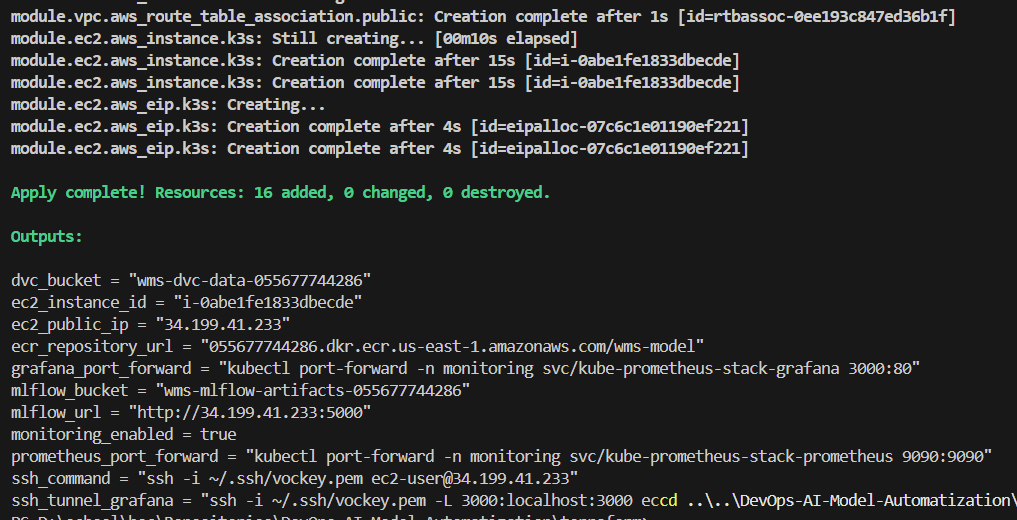
\includegraphics[width=\linewidth]{img/06_wdrozenie_systemu/terraform_apply.png}
  \caption{Wynik polecenia \texttt{terraform apply} --- lista 12 utworzonych zasobów AWS}
  \label{fig:terraform-apply}
\end{figure}

Rysunki~\ref{fig:aws-ec2} i~\ref{fig:aws-s3} przedstawiają odpowiednio instancję EC2 i zasobniki S3 w konsoli AWS.

\begin{figure}[H]
  \centering
  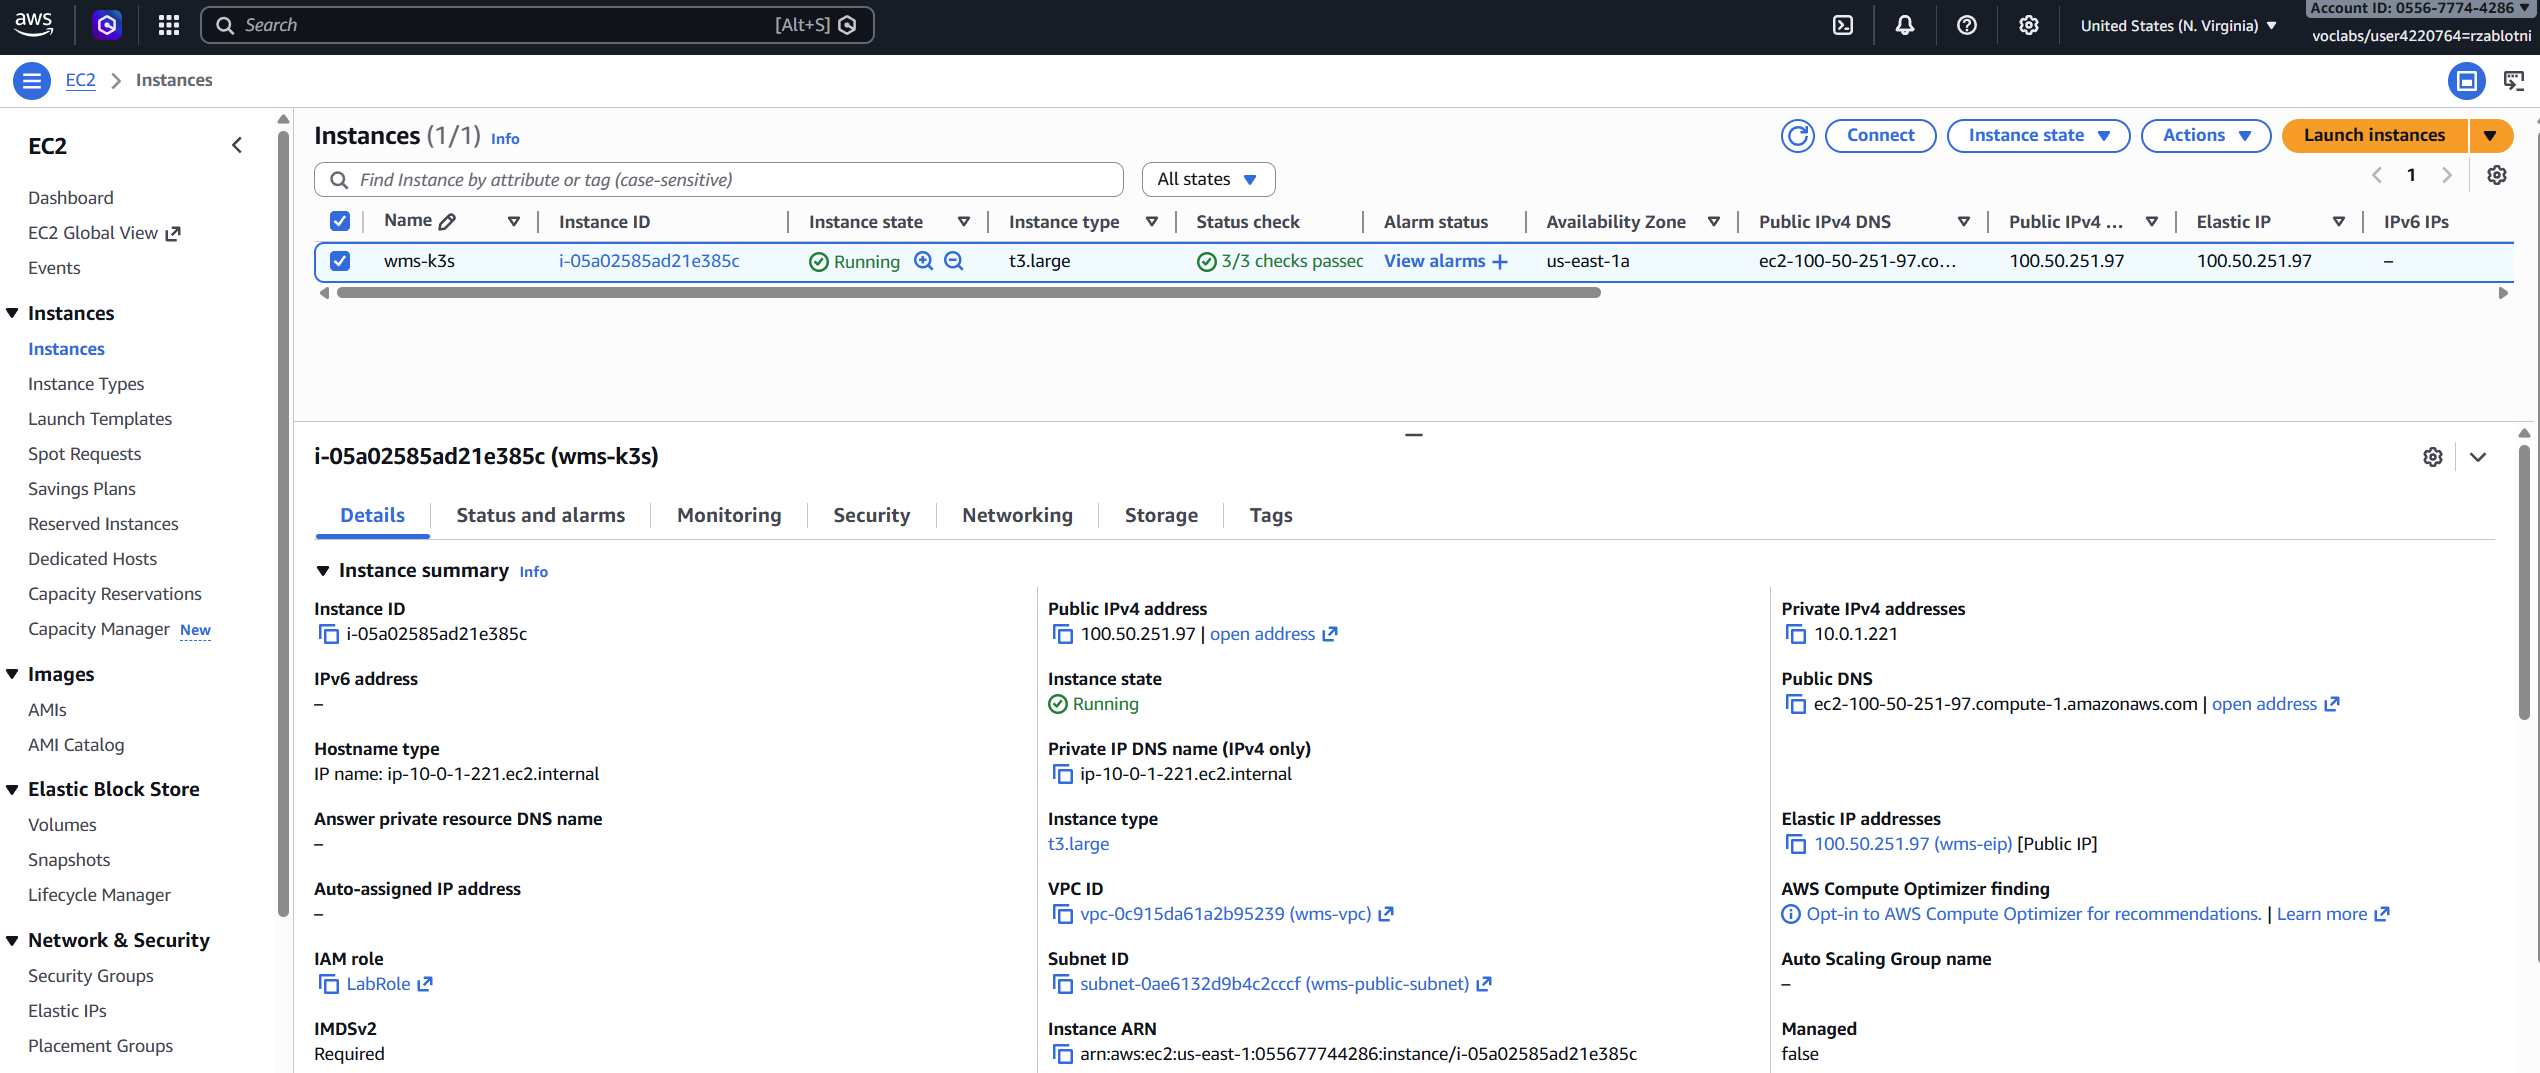
\includegraphics[width=\linewidth]{img/06_wdrozenie_systemu/aws_ec2_console.png}
  \caption{Instancja EC2 \texttt{wms-k3s} w konsoli AWS}
  \label{fig:aws-ec2}
\end{figure}
\vspace{-30pt}
\begin{figure}[H]
  \centering
  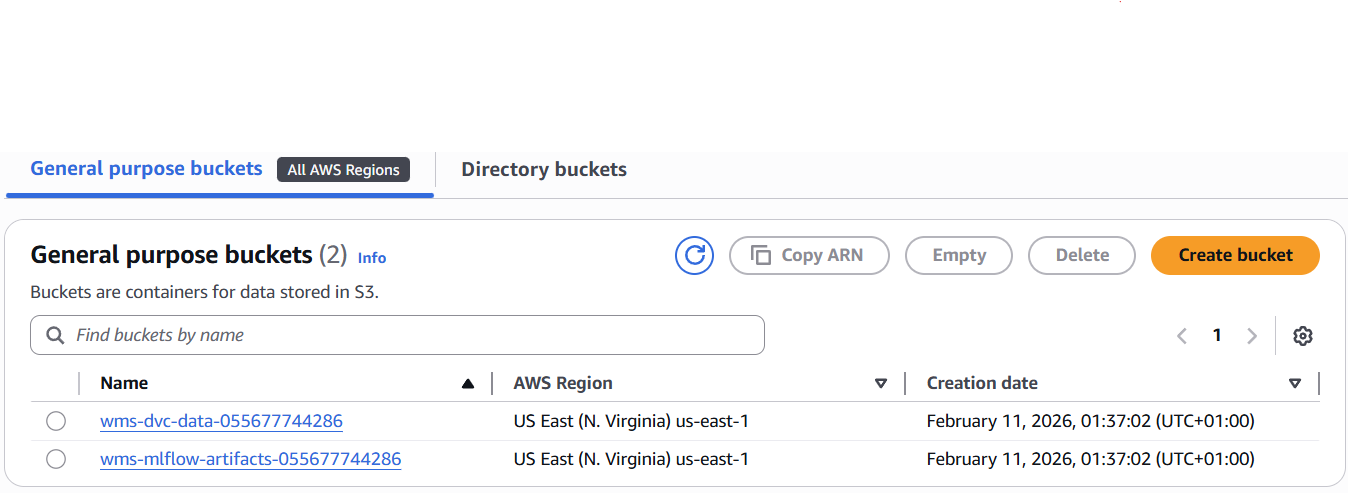
\includegraphics[width=\linewidth]{img/06_wdrozenie_systemu/aws_s3_buckets.png}
  \caption{Zasobniki S3: \texttt{wms-dvc-data-*} dla danych treningowych i \texttt{wms-mlflow-artifacts-*} dla artefaktów}
  \label{fig:aws-s3}
\end{figure}
\vspace{5pt}

\subsection{Konfiguracja EC2 i k3s}

Konfiguracja instancji EC2 odbywa się automatycznie przy pierwszym uruchomieniu za pomocą skryptu \texttt{user-data}. Skrypt jest szablonowany przez Terraform, który przy generowaniu pliku podstawiane są zmienne takie jak adres zasobnika S3 i region AWS, dzięki czemu nie ma żadnych wartości zakodowanych na stałe.

Kroki wykonywane przez \texttt{user-data}:
\begin{enumerate}
  \item Instalacja zależności systemowych: \texttt{dnf install -y git curl libicu}.
  \item Instalacja k3s --- uproszczonego Kubernetes \cite{k3s_docs}.
  \item Instalacja MLflow i boto3: \texttt{pip3 install --ignore-installed mlflow boto3}.
  \item Konfiguracja MLflow jako usługi systemd:
\begin{verbatim}
[Service]
ExecStart=mlflow server \
  --host 0.0.0.0 --port 5000 \
  --default-artifact-root s3://${mlflow_bucket}/
\end{verbatim}
  \item Instalacja GitHub Actions runnera jako usługi systemd.
\end{enumerate}

Instancja korzysta z Amazon Linux 2023, który oferuje nowszy OpenSSL 3.0 i wsparcie producenta do 2028 roku. Po zakończeniu \texttt{user-data} instancja jest gotowa do przyjęcia zadań z GitHub Actions bez dalszej konfiguracji ręcznej.

\textbf{Architektura k3s.} K3s to uproszczona dystrybucja Kubernetes zawarta w pojedynczym pliku binarnym. W porównaniu do pełnego Kubernetes zastępuje etcd bazą SQLite, usuwa przestarzałe sterowniki i wbudowuje podstawowe komponenty sieciowe. Dzięki temu działa na instancji \texttt{t3.large} (8~GB RAM) ze znaczącym zapasem zasobów dla poda z modelem; pełne Kubernetes samo w sobie wymagałoby podobnej ilości RAM.

W projekcie użyty jest klaster jednorazłowy (single-node): jeden węzeł pełni jednocześnie rolę control plane i workera. Taka architektura jest wystarczająca dla jednej działającej aplikacji i eliminuje koszty dodatkowych instancji EC2. Wysoka dostępność (HA) nie była wymaganiem. System jest przeznaczony do demonstracji i testowania, nie do środowiska produkcyjnego.

\textbf{Strategia aktualizacji.} Dla Deploymentu zastosowano domyślną strategię \texttt{RollingUpdate}: k3s najpierw uruchamia nowy pod, a dopiero po jego gotowości usuwa stary. Oznacza to zerowy przestój (zero-downtime deployment) przy aktualizacji modelu. Działa to jednak tylko wtedy, gdy instancja EC2 jest uruchomiona. W przeciwnym wypadku klaster jest niedostępny.

\textbf{Rollbacki i wersjonowanie.} Rollbacki na poziomie Kubernetes nie są rozbudowane celowo. Mechanizmem wersjonowania modeli jest MLflow, gdzie każda wersja modelu jest zarejestrowana w rejestrze MLflow ze swoimi metrykami. Rollback polega na przestawieniu stadium modelu w MLflow z \texttt{Production} na poprzednią wersję i ponownym uruchomieniu \texttt{deploy-model.yaml}. Helm zachowuje historię ostatnich wdrożeń (\texttt{helm history wms-api}), co umożliwia też cofnięcie konfiguracji Kubernetes bez ponownego treningu.

Rysunek~\ref{fig:systemctl-status} potwierdza poprawne działanie usług systemd, a rysunek~\ref{fig:kubectl-pods} przedstawia aktualny stan podów klastra k3s.

\begin{figure}[H]
 \centering
  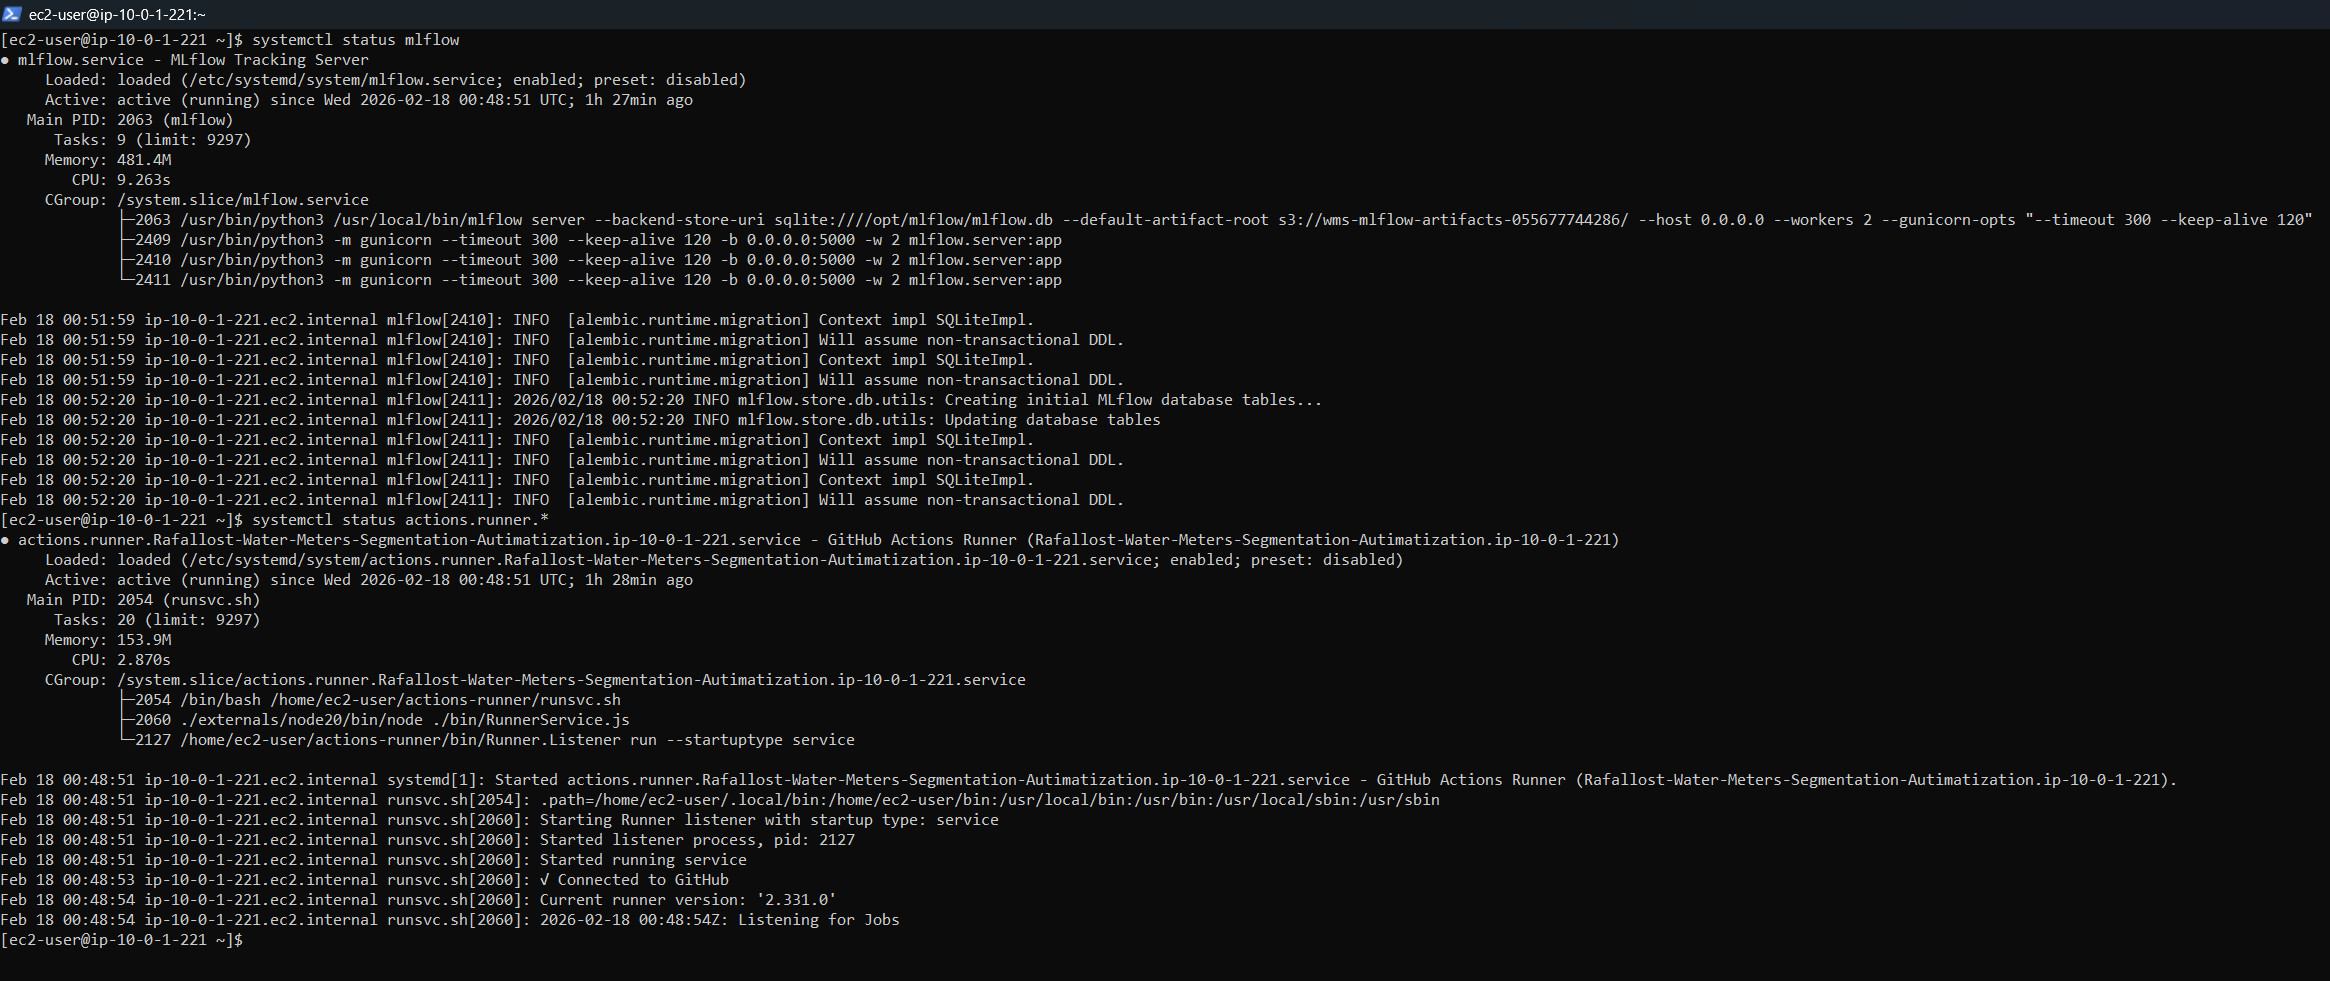
\includegraphics[width=\linewidth]{img/06_wdrozenie_systemu/systemctl_status.png}
  \caption{Stan usług \texttt{mlflow} i \texttt{actions.runner} w systemd --- obie usługi aktywne}
  \label{fig:systemctl-status}
\end{figure}

\begin{figure}[H]
 \centering
  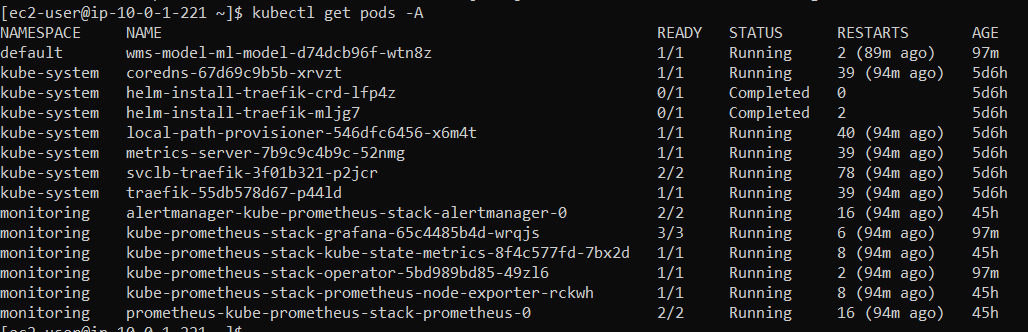
\includegraphics[width=\linewidth]{img/06_wdrozenie_systemu/kubectl_pods.png}
  \caption{Pody klastra k3s --- \texttt{kubectl get pods -A}. Widoczny pod API modelu oraz stos monitorowania.}
  \label{fig:kubectl-pods}
\end{figure}

Interfejs MLflow dostępny jest pod adresem \texttt{http://100.50.251.97:5000} (rys.~\ref{fig:mlflow-ui}).

\begin{figure}[H]
 \centering
 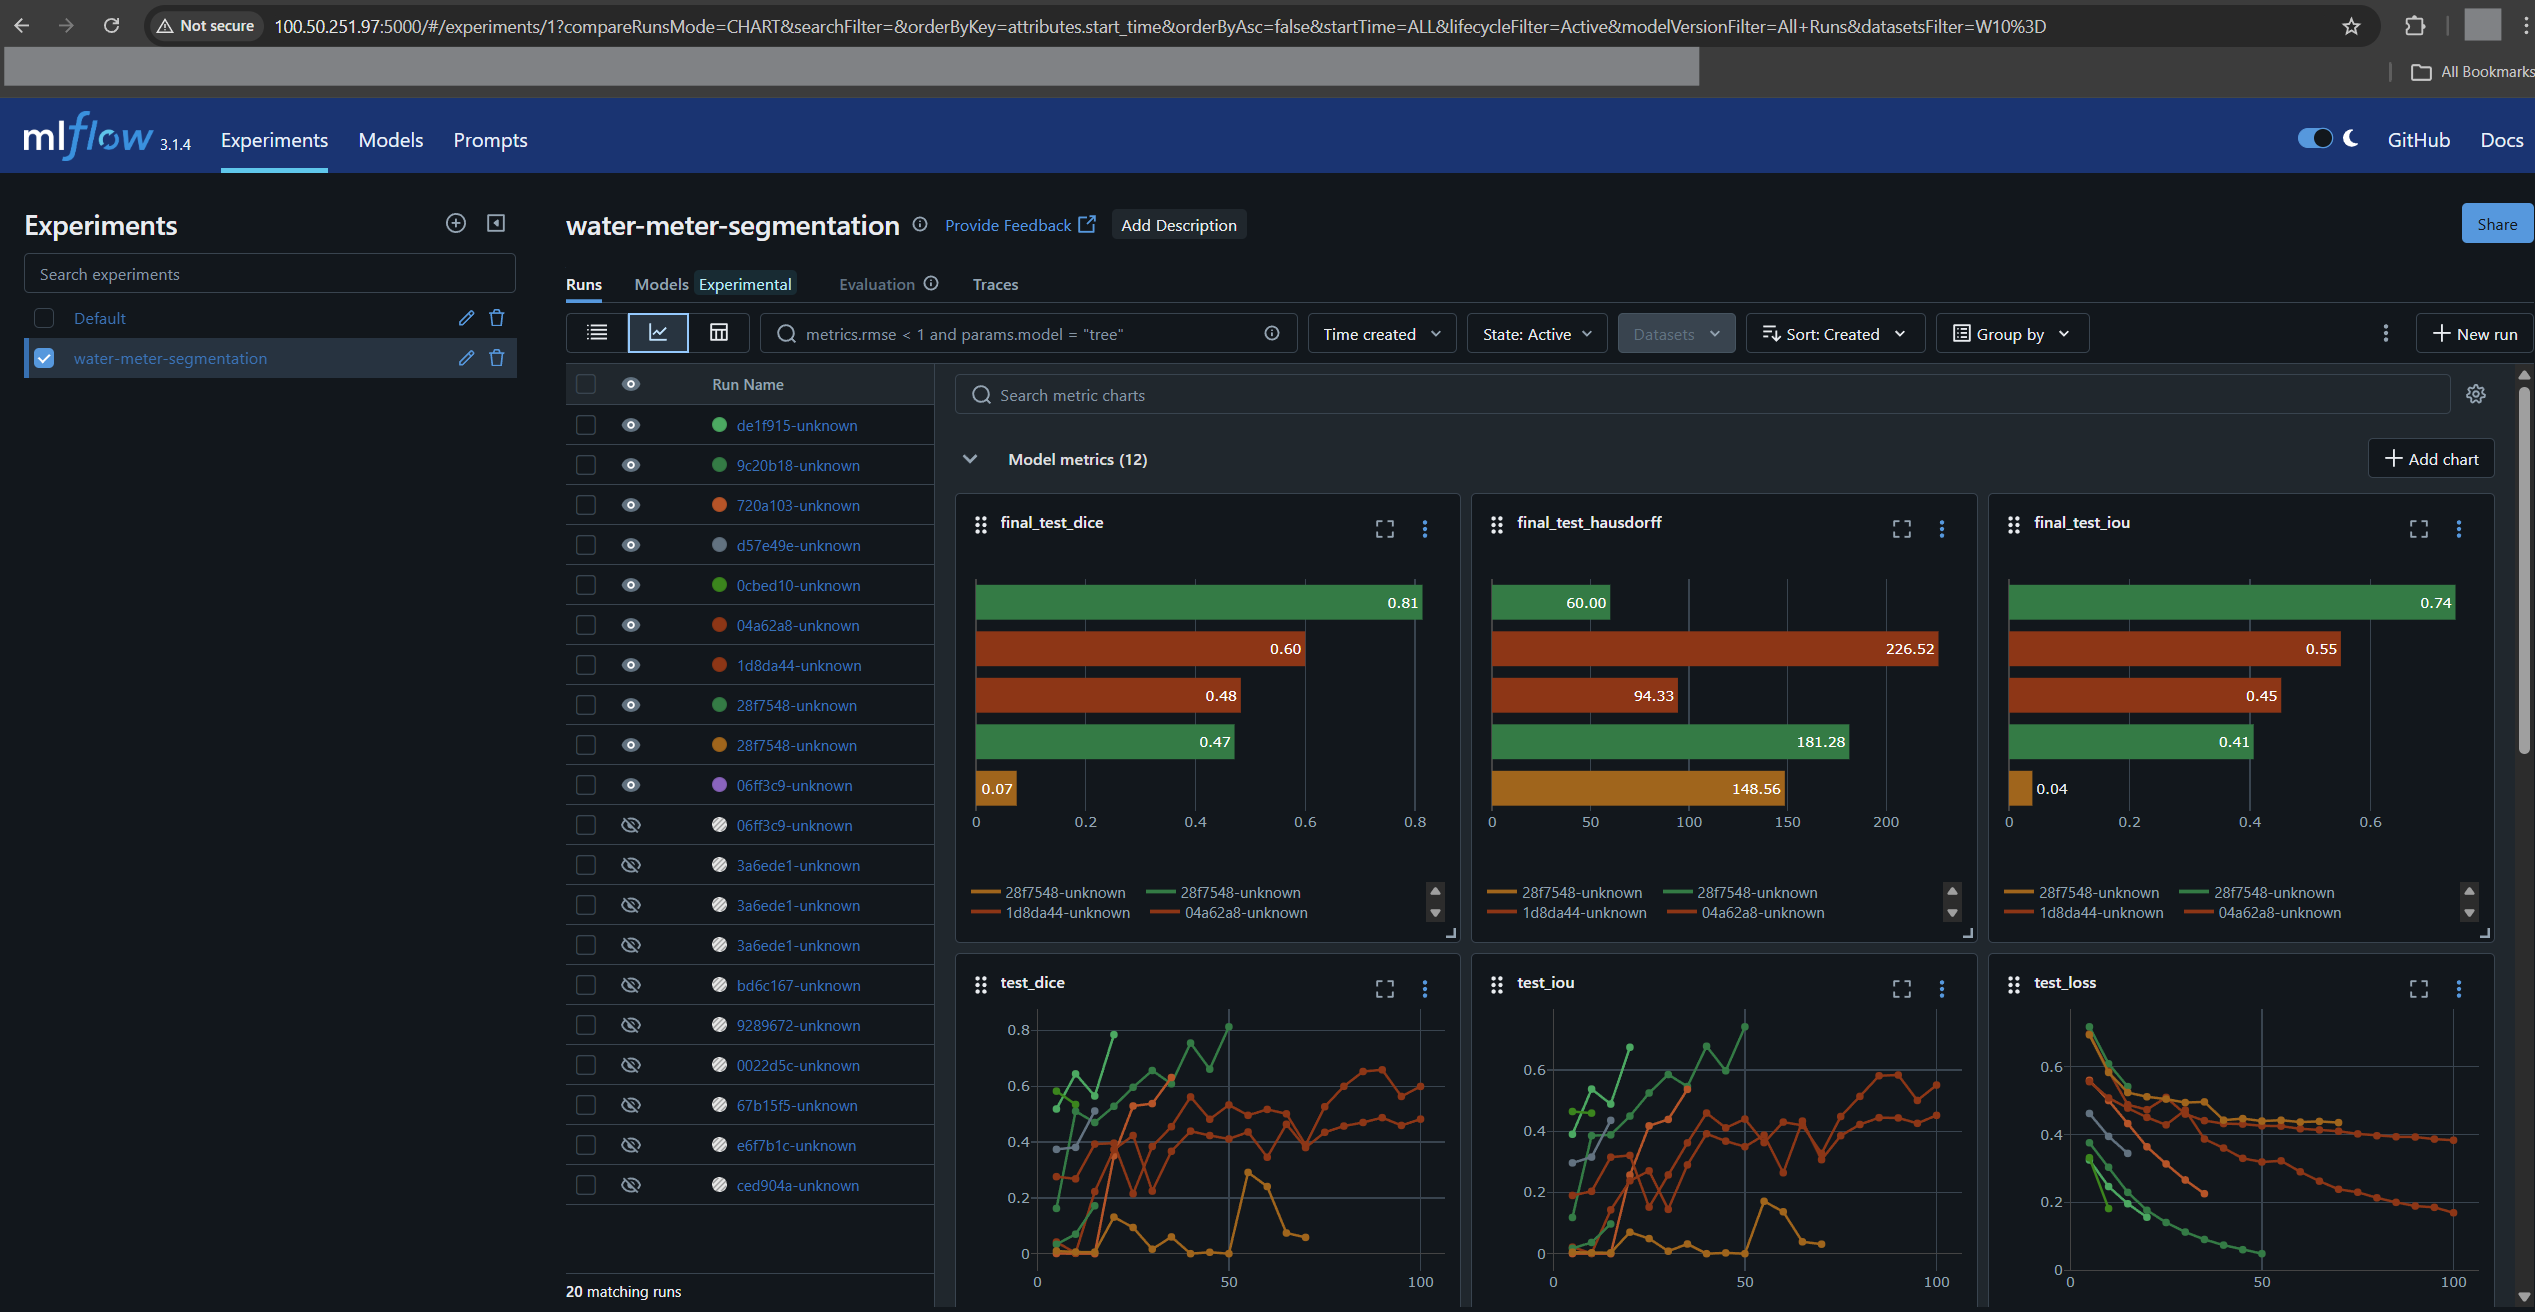
\includegraphics[width=\linewidth]{img/06_wdrozenie_systemu/mlflow_ui.png}
 \caption{Interfejs MLflow (\texttt{http://100.50.251.97:5000}) --- lista eksperymentów i przebiegów treningowych z metrykami}
 \label{fig:mlflow-ui}
\end{figure}

\subsection{Dostępne porty i usługi}
\label{subsec:porty}

Security Group Terraform otwiera wyłącznie porty niezbędne do działania systemu. Tabela~\ref{tab:ports} zestawia wszystkie dostępne punkty dostępu.

\begin{table}[H]
\centering
\caption{Porty dostępne na instancji EC2 \texttt{wms-k3s}}
\label{tab:ports}
\begin{tabular}{|c|l|l|}
\hline
\textbf{Port} & \textbf{Usługa} & \textbf{Przeznaczenie} \\
\hline
22   & SSH             & Zarządzanie instancją EC2 (tylko IP operatora) \\
\hline
5000 & MLflow          & Interfejs śledzenia eksperymentów i rejestr modeli \\
\hline
30080 & API modelu (NodePort) & Predykcja segmentacji --- endpoint \texttt{/predict} \\
\hline
30300 & Grafana (NodePort)    & Dashboard wizualizacji metryk \\
\hline
30900 & Prometheus (NodePort) & Interfejs zapytań i podgląd \textit{Targets} \\
\hline
\end{tabular}
\end{table}

Ruch przychodzący na porty 5000, 30080, 30300 i 30900 jest dozwolony z dowolnego adresu IP (\texttt{0.0.0.0/0}), ponieważ EC2 nie jest wyposażone w Load Balancer z certyfikatem TLS, a połączenia odbywają się po HTTP. Port SSH (22) jest ograniczony do konkretnego adresu IP operatora skonfigurowanego w \texttt{terraform.tfvars}. Konfigurację Security Group przedstawia rysunek~\ref{fig:security-group}.

\begin{figure}[H]
  \centering
  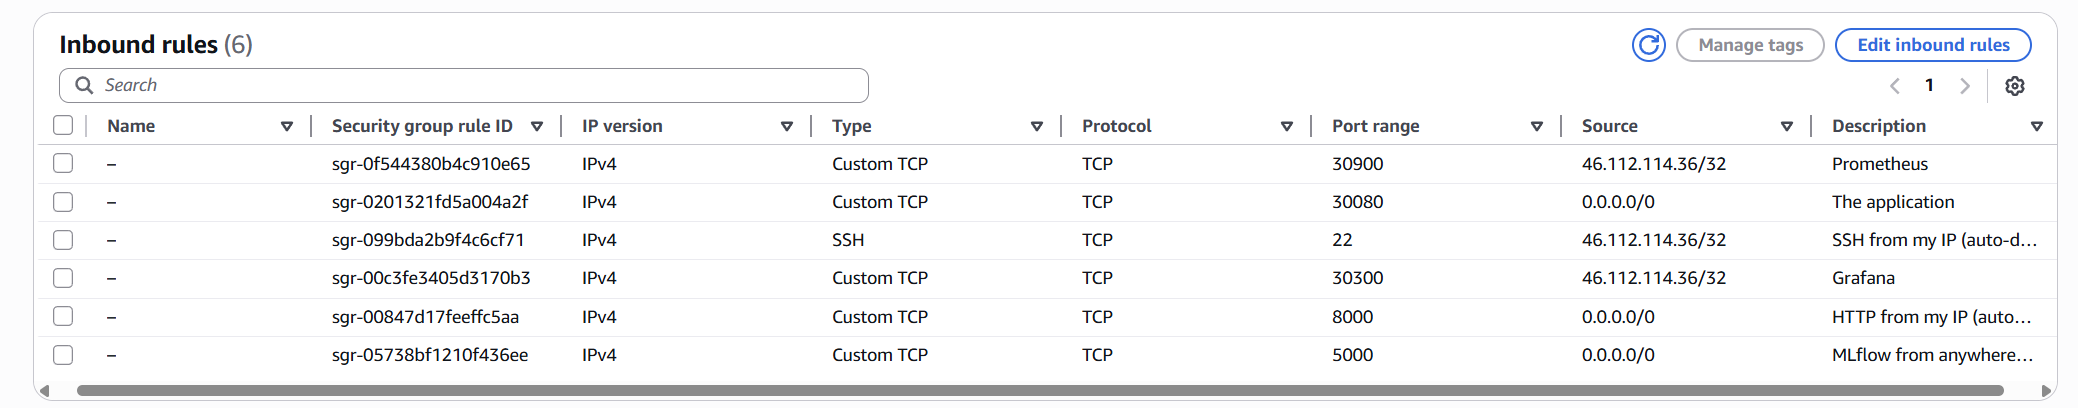
\includegraphics[width=\linewidth]{img/06_wdrozenie_systemu/security_groups.png}
  \caption{Security Group instancji EC2 --- reguły ruchu przychodzącego z otwartymi portami usług}
  \label{fig:security-group}
\end{figure}

\subsection{Konfiguracja Helm}

W projekcie Helm \cite{helm_docs} wykorzystywany jest dwojako: do wdrożenia własnego charta API modelu oraz do konfiguracji zewnętrznego stosu monitorowania.

\textbf{Chart API modelu.} Katalog \texttt{devops/helm/ml-model/} zawiera własny chart Kubernetes dla serwera API. Zamiast zarządzać oddzielnymi plikami manifestów, całą aplikację opisuje jeden zestaw szablonów YAML sparametryzowanych zmiennymi. Bez Helm każda aktualizacja wymagałaby ręcznej edycji kilku plików i kolejnych wywołań \texttt{kubectl apply}. Helm sprowadza to do jednej komendy:

\begin{verbatim}
helm upgrade --install wms-model devops/helm/ml-model/ \
  -f infrastructure/helm-values.yaml \
  --namespace default --create-namespace
\end{verbatim}

Komenda ta działa zarówno przy pierwszym wdrożeniu (\textit{install}) jak i przy aktualizacji (\textit{upgrade}); Helm sam sprawdza czy release już istnieje. Helm zachowuje historię wdrożeń (\texttt{helm history wms-model}), co umożliwia szybki rollback do poprzedniej wersji.

Struktura charta:

\begin{verbatim}
devops/helm/ml-model/
+-- Chart.yaml              <- metadane (nazwa, wersja charta)
+-- values.yaml             <- wartosci domyslne (NodePort 30080, limity RAM/CPU)
\-- templates/
    +-- _helpers.tpl        <- funkcje pomocnicze Helm
    +-- deployment.yaml     <- zasob Deployment
    +-- service.yaml        <- zasob Service (NodePort 30080)
    \-- servicemonitor.yaml <- ServiceMonitor dla Prometheus
\end{verbatim}

Szablony korzystają ze składni Go Templates i odwołują się do wartości przez \texttt{.Values.*}. Plik \texttt{infrastructure/helm-values.yaml} nadpisuje wartości domyślne charta dla konkretnego wdrożenia. Najważniejsze fragmenty:

\begin{verbatim}
image:
  repository: "055677744286.dkr.ecr.us-east-1.amazonaws.com/wms-model"
  pullPolicy: Always
  tag: "latest"

imagePullSecrets:
  - name: ecr-secret    # dane do logowania do ECR

env:
  - name: MLFLOW_TRACKING_URI
    value: "http://localhost:5000"  # MLflow na hoscie EC2 (hostNetwork)
  - name: MODEL_VERSION
    value: "production"

resources:
  limits:
    memory: "1Gi"
    cpu: "500m"
  requests:
    memory: "512Mi"
    cpu: "100m"
\end{verbatim}

Warto zwrócić uwagę na \texttt{MLFLOW\_TRACKING\_URI: localhost:5000}; kontener korzysta z \texttt{hostNetwork: true}, co pozwala mu odwoływać się do MLflow działającego bezpośrednio na maszynie EC2, bez konieczności dodatkowej usługi Kubernetes. Przy każdym wdrożeniu GitHub Actions podaje aktualny hash commita jako \texttt{--set image.tag=\$\{COMMIT\_SHA\}}, co zapewnia jednoznaczną identyfikację wersji obrazu.

Postęp wdrożenia API można śledzić w czasie rzeczywistym poleceniem:
\begin{verbatim}
kubectl rollout status deployment/wms-model-ml-model --watch
\end{verbatim}

Po wdrożeniu API jest dostępne pod adresem \texttt{http://100.50.251.97:30080}.

\begin{figure}[H]
 \centering
 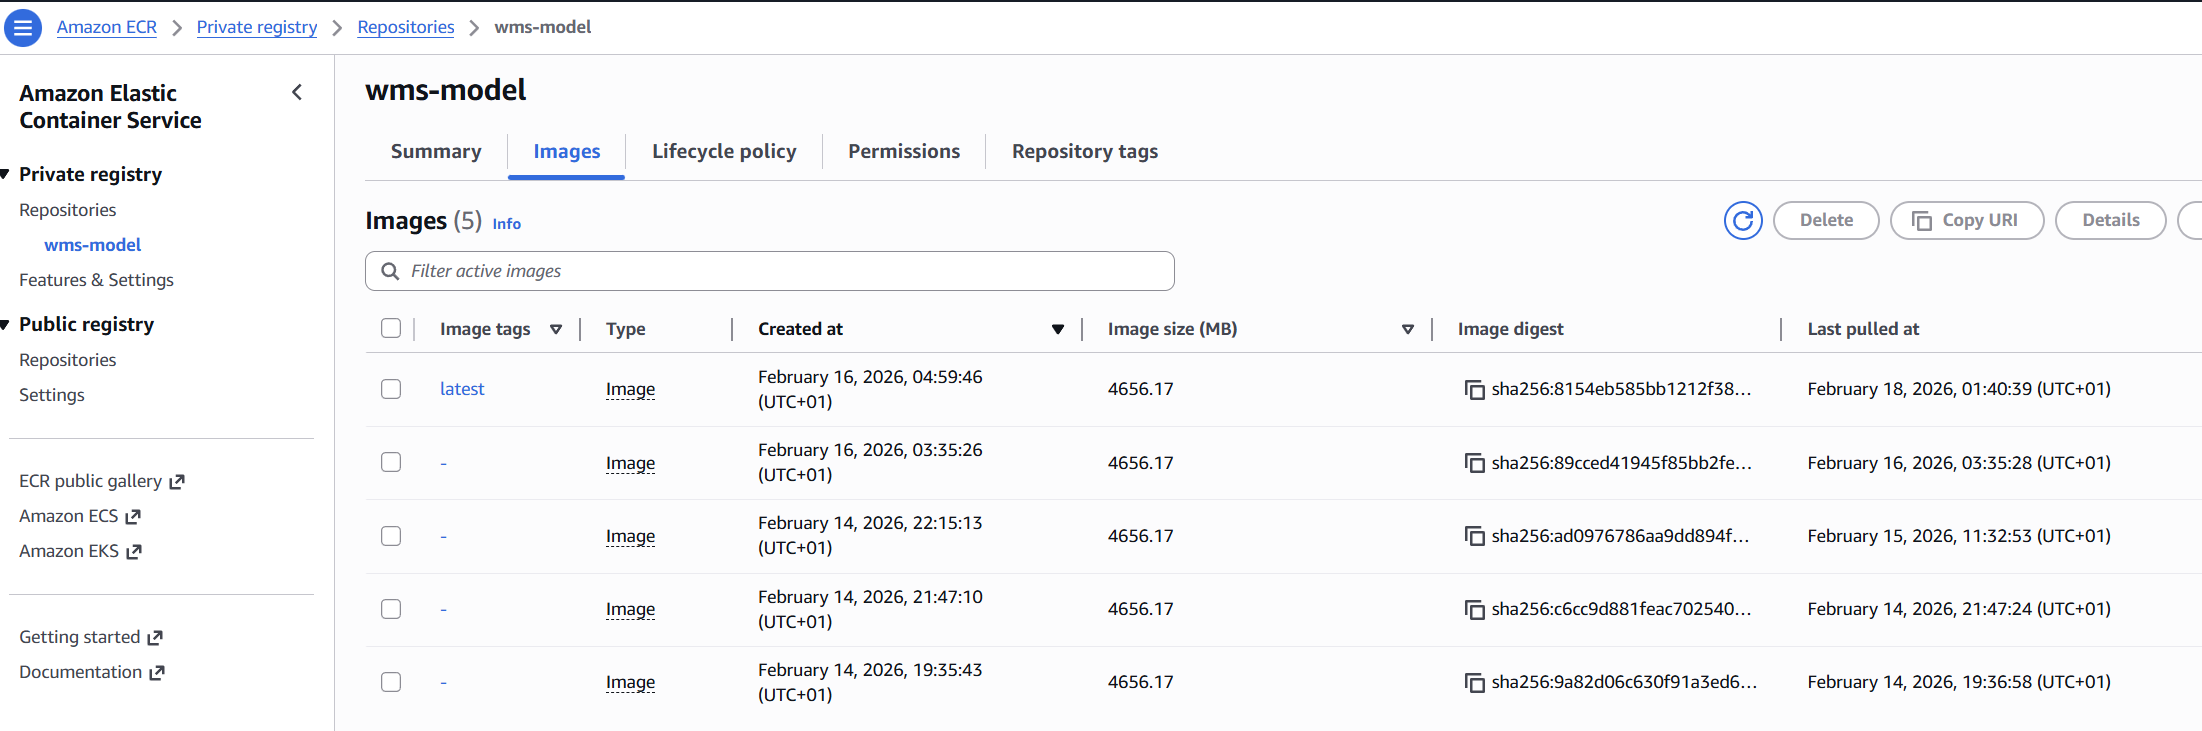
\includegraphics[width=0.9\linewidth]{img/06_wdrozenie_systemu/ecr_repository.png}
 \caption{Repozytorium \texttt{wms-model} w Amazon ECR z obrazami oznaczonymi hashiem commita}
 \label{fig:ecr-repo}
\end{figure}

Dostępne endpointy API to \texttt{/health} (status usługi), \texttt{/predict} (predykcja segmentacji) i \texttt{/metrics} (metryki Prometheus). Odpowiedź endpointu \texttt{/health} przedstawia rysunek~\ref{fig:api-health}, a pełną listę eksponowanych metryk prezentuje rysunek~\ref{fig:metrics}.

\begin{figure}[H]
  \centering
  \begin{subfigure}[t]{0.48\linewidth}
    \centering
    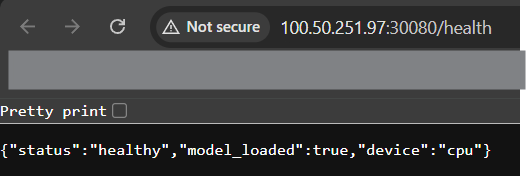
\includegraphics[width=\linewidth]{img/06_wdrozenie_systemu/api_health.png}
    \caption{Odpowiedź endpointu \texttt{/health} wdrożonego API modelu}
    \label{fig:api-health}
  \end{subfigure}
  \hfill
  \begin{subfigure}[t]{0.48\linewidth}
    \centering
    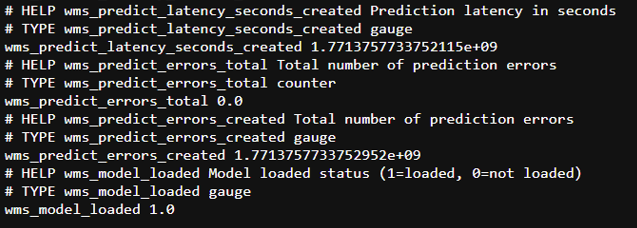
\includegraphics[width=\linewidth]{img/06_wdrozenie_systemu/metrics_short.png}
    \caption{Metryki Prometheus eksponowane pod adresem \texttt{/metrics}: liczba predykcji, czasy odpowiedzi i błędy}
    \label{fig:metrics}
  \end{subfigure}
  \caption{Endpointy diagnostyczne API modelu}
  \label{fig:api-endpoints}
\end{figure}

\subsection{Stos monitorowania}

Monitoring oparty na Prometheus \cite{prometheus_docs} i Grafana wdrażany jest jako oddzielny stos na tym samym klastrze k3s. Składa się z trzech komponentów:

\begin{itemize}
  \item \textbf{Prometheus} --- zbiera metryki z endpointu \texttt{/metrics} API modelu co 15 sekund; konfiguracja scraping w \texttt{prometheus.yml},
  \item \textbf{Grafana} --- wizualizuje metryki na predefiniowanych dashboardach; dostępna na porcie NodePort 30300,
  \item \textbf{kube-state-metrics} --- dostarcza metryki Kubernetes (stan podów, zużycie zasobów węzła).
\end{itemize}

\begin{sloppypar}
API modelu eksponuje metryki w formacie Prometheus przy użyciu biblioteki \texttt{prometheus\_client}. Śledzone metryki to:
\end{sloppypar}
\begin{itemize}
  \item \texttt{wms\_predictions\_total} --- łączna liczba żądań predykcji (Counter),
  \item \texttt{wms\_predict\_latency\_seconds} --- histogram czasów odpowiedzi,
  \item \texttt{wms\_predict\_errors\_total} --- liczba błędów (Counter),
  \item \texttt{wms\_model\_loaded} --- czy model jest załadowany (Gauge, wartość 0 lub 1).
\end{itemize}

Działanie stosu monitorowania ilustruje dashboard Grafana (rys.~\ref{fig:grafana-dashboard}) oraz widok Targets w Prometheus (rys.~\ref{fig:prometheus-targets}).

\begin{figure}[H]
 \centering
 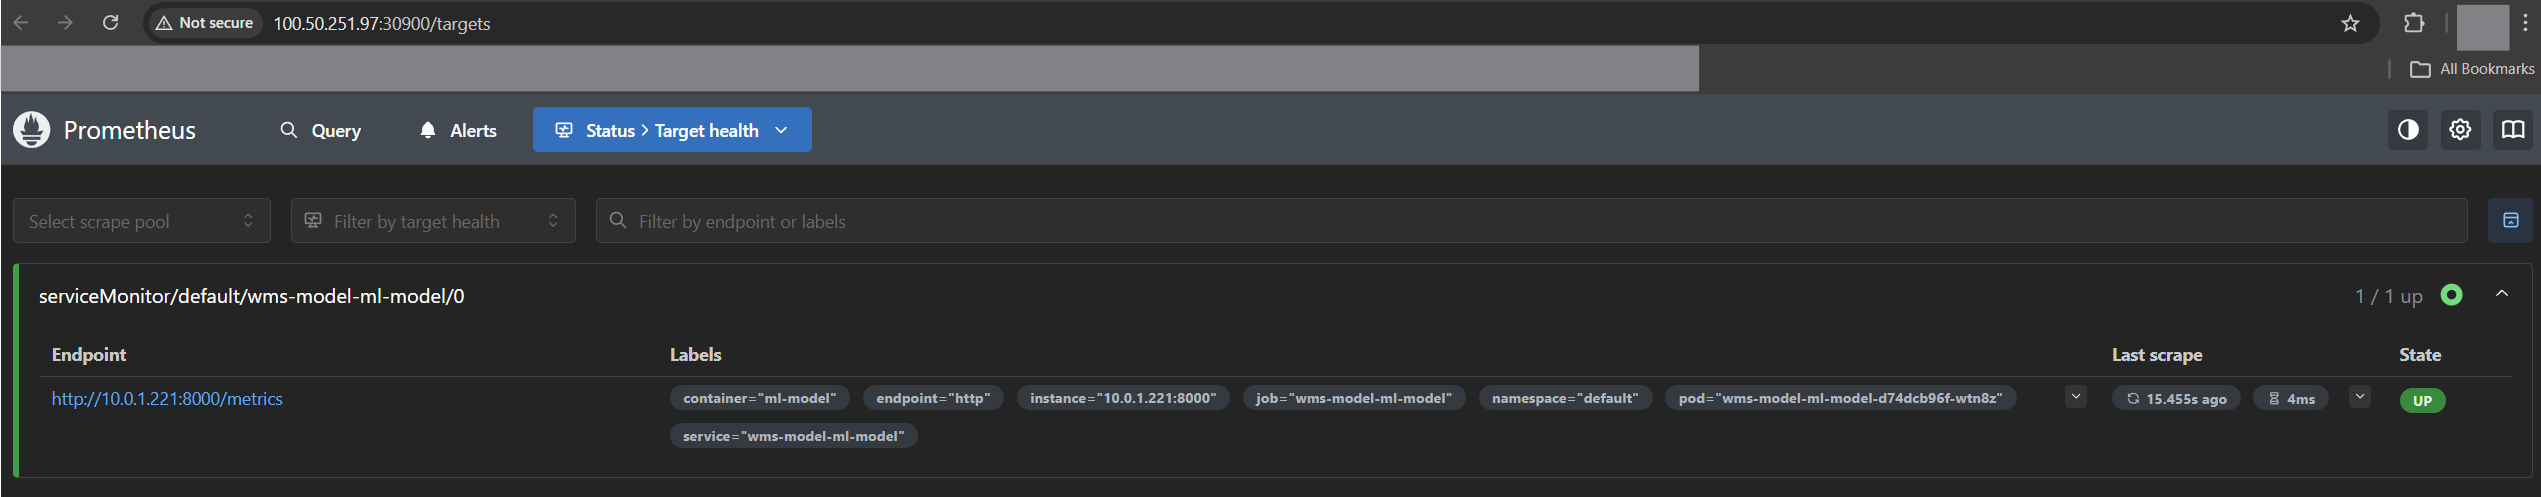
\includegraphics[width=\linewidth]{img/06_wdrozenie_systemu/prometheus_targets.png}
 \caption{Strona \textit{Targets} w Prometheus (\texttt{:30900}) --- endpoint \texttt{/metrics} API w stanie \texttt{UP}}
 \label{fig:prometheus-targets}
\end{figure}

\begin{figure}[H]
 \centering
 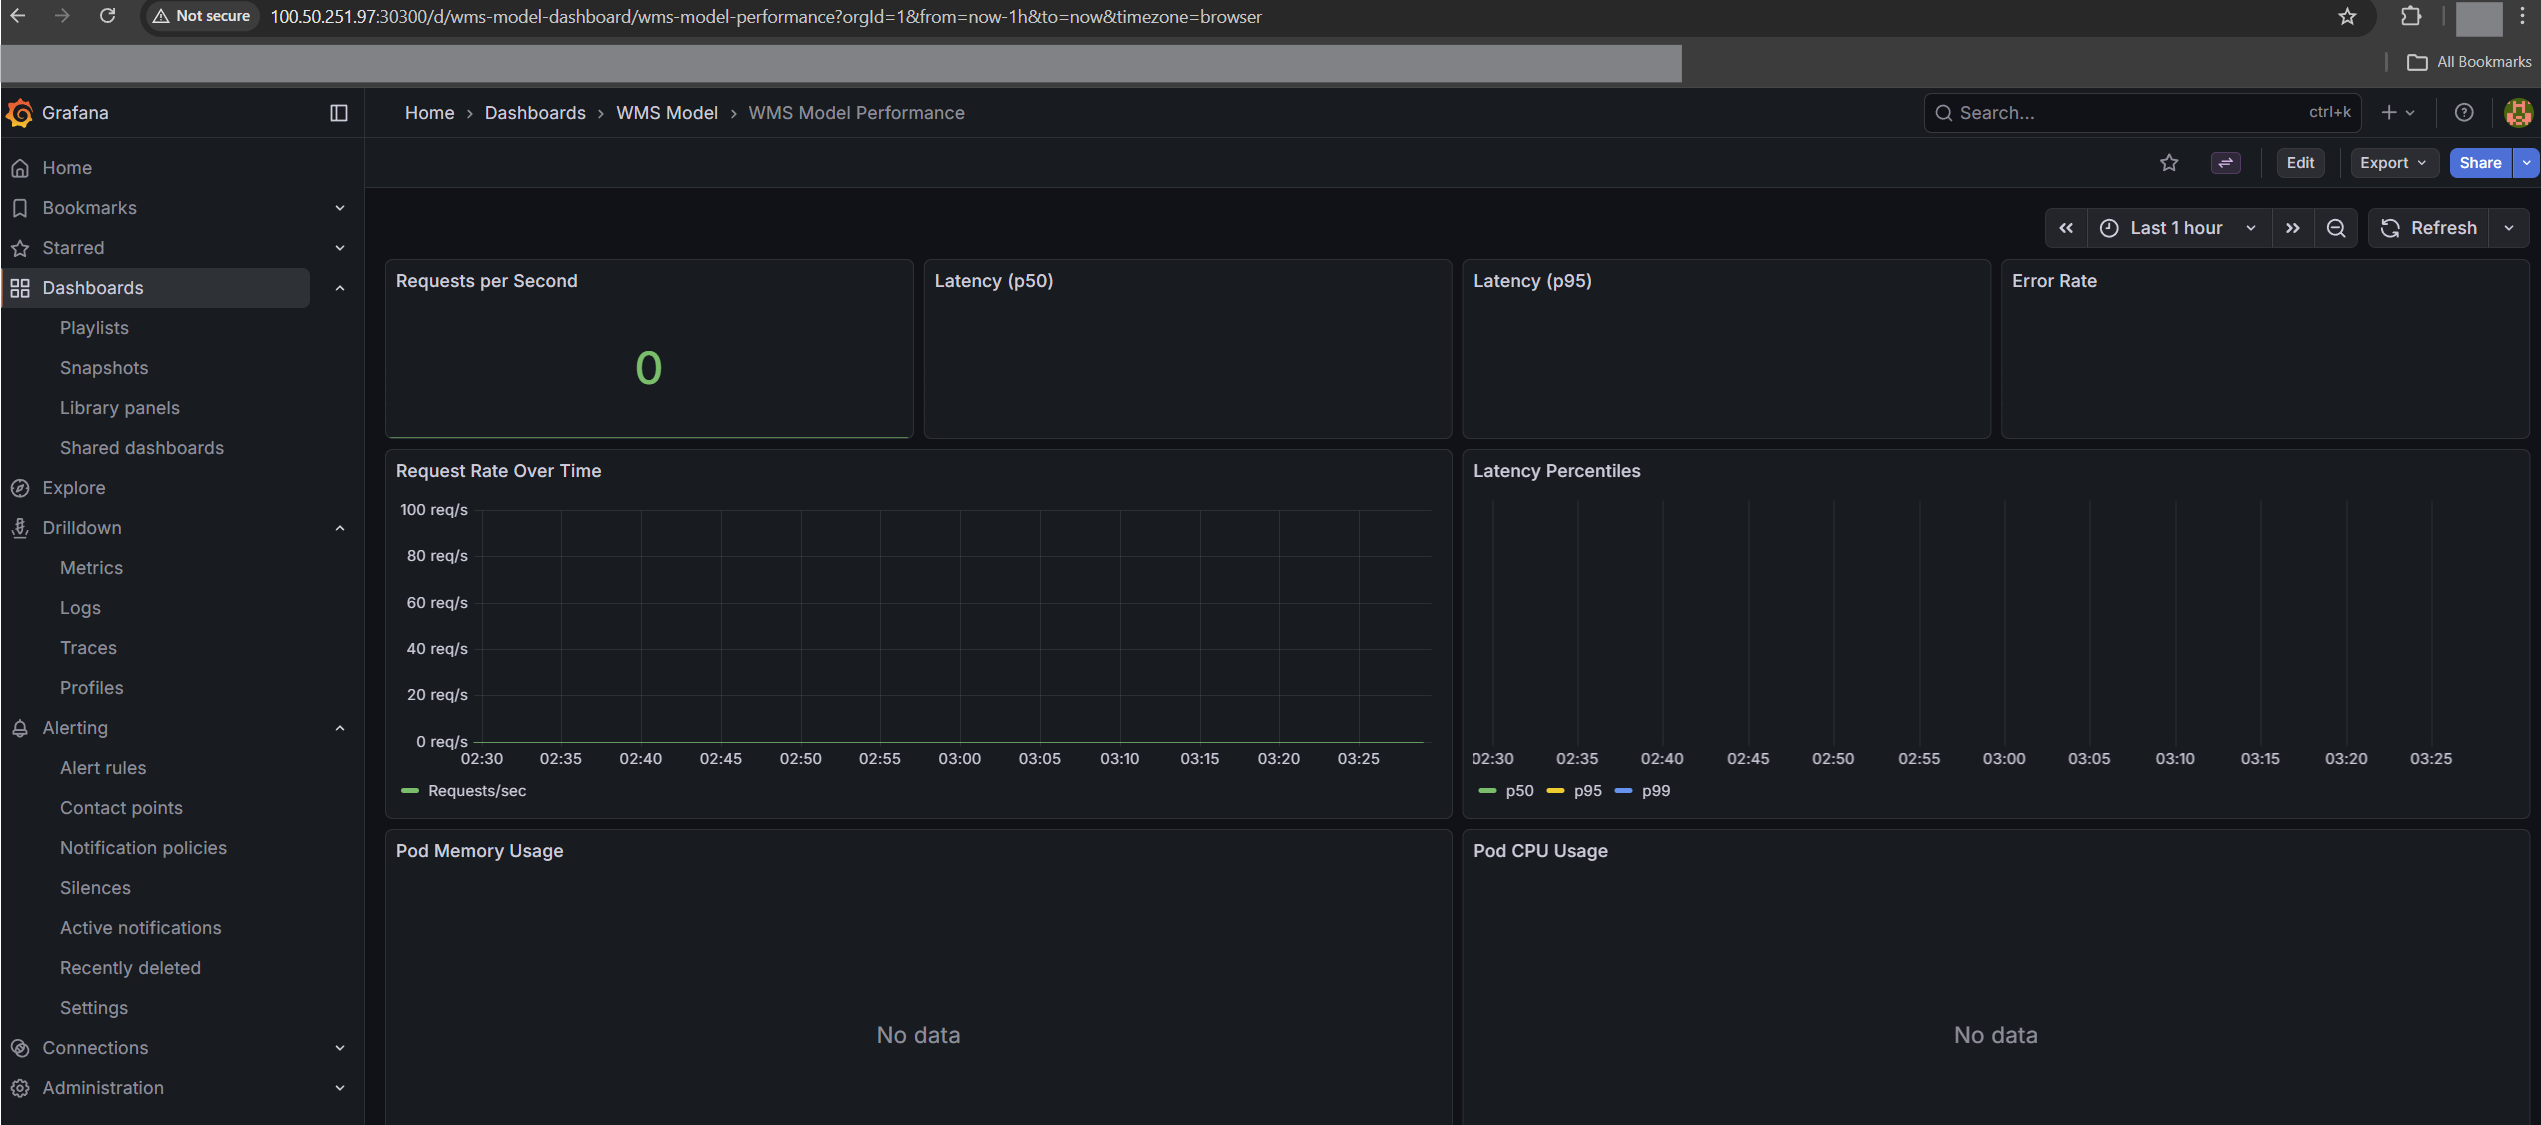
\includegraphics[width=\linewidth]{img/06_wdrozenie_systemu/grafana_dashboard.png}
 \caption{Dashboard Grafana (\texttt{http://100.50.251.97:30300}) --- metryki działającego API modelu}
 \label{fig:grafana-dashboard}
\end{figure}

\subsection{Workflow użytkownika}

\subsubsection{Scenariusz 1: Wdrożenie przez automatyczny pipeline}

Jak opisano w rozdziale~\ref{sec:Pipeline_CICD}, dostarczenie nowych danych treningowych przez \texttt{git push} wyzwala pełny pipeline. Jeśli wytrenowany model przeszedł bramkę jakości, pipeline automatycznie wdraża go na klaster k3s przez \texttt{deploy-model.yaml}, a następnie zatrzymuje instancję EC2. Po zakończeniu pipeline'u aplikacja jest zainstalowana na klastrze i gotowa do działania. Aby skorzystać z API, wystarczy uruchomić instancję EC2 za pomocą workflow \textit{Manual EC2 Control} (zakładka \textit{Actions} w GitHub, akcja \textit{start}). Po uruchomieniu workflow wyświetla adres IP w podsumowaniu, a endpoint \texttt{/predict} jest natychmiast dostępny.

Należy zaznaczyć, że wdrożenie następuje tylko gdy model poprawił metryki. Jeśli trening nie przeszedł bramki jakości, klaster k3s nadal serwuje poprzednią wersję. Do kontrolowanego wdrożenia niezależnego od treningu służy Scenariusz~2.

\subsubsection{Scenariusz 2: Ręczne wdrożenie i korzystanie z API (zalecany)}

Jest to zalecany sposób korzystania z systemu dla operatora chcącego uruchomić lub zaktualizować działające API. Cały proces odbywa się przez interfejs GitHub Actions i nie wymaga żadnych lokalnych poświadczeń AWS.

\textbf{Krok 1: Wdrożenie modelu.} W zakładce \textit{Actions} należy uruchomić workflow \textit{Release \& Deploy} (\texttt{release-deploy.yaml}) klikając \textit{Run workflow}. Workflow automatycznie uruchamia instancję EC2, buduje obraz Docker, wypycha go do ECR, pobiera najnowszy model ze stadium Production z MLflow, aktualizuje klaster k3s przez Helm, a po weryfikacji zatrzymuje EC2.

\textbf{Krok 2: Uruchomienie instancji do predykcji.} Po wdrożeniu model jest zainstalowany na klastrze, ale EC2 jest zatrzymany w celu oszczędności. Aby wysyłać zapytania do API, należy uruchomić instancję workflow \textit{Manual EC2 Control} z akcją \textit{start}. Workflow wyświetla aktualne IP i URL MLflow w podsumowaniu uruchomienia. API jest dostępne pod adresem \texttt{http://100.50.251.97:30080/}.

\begin{figure}[H]
  \centering
  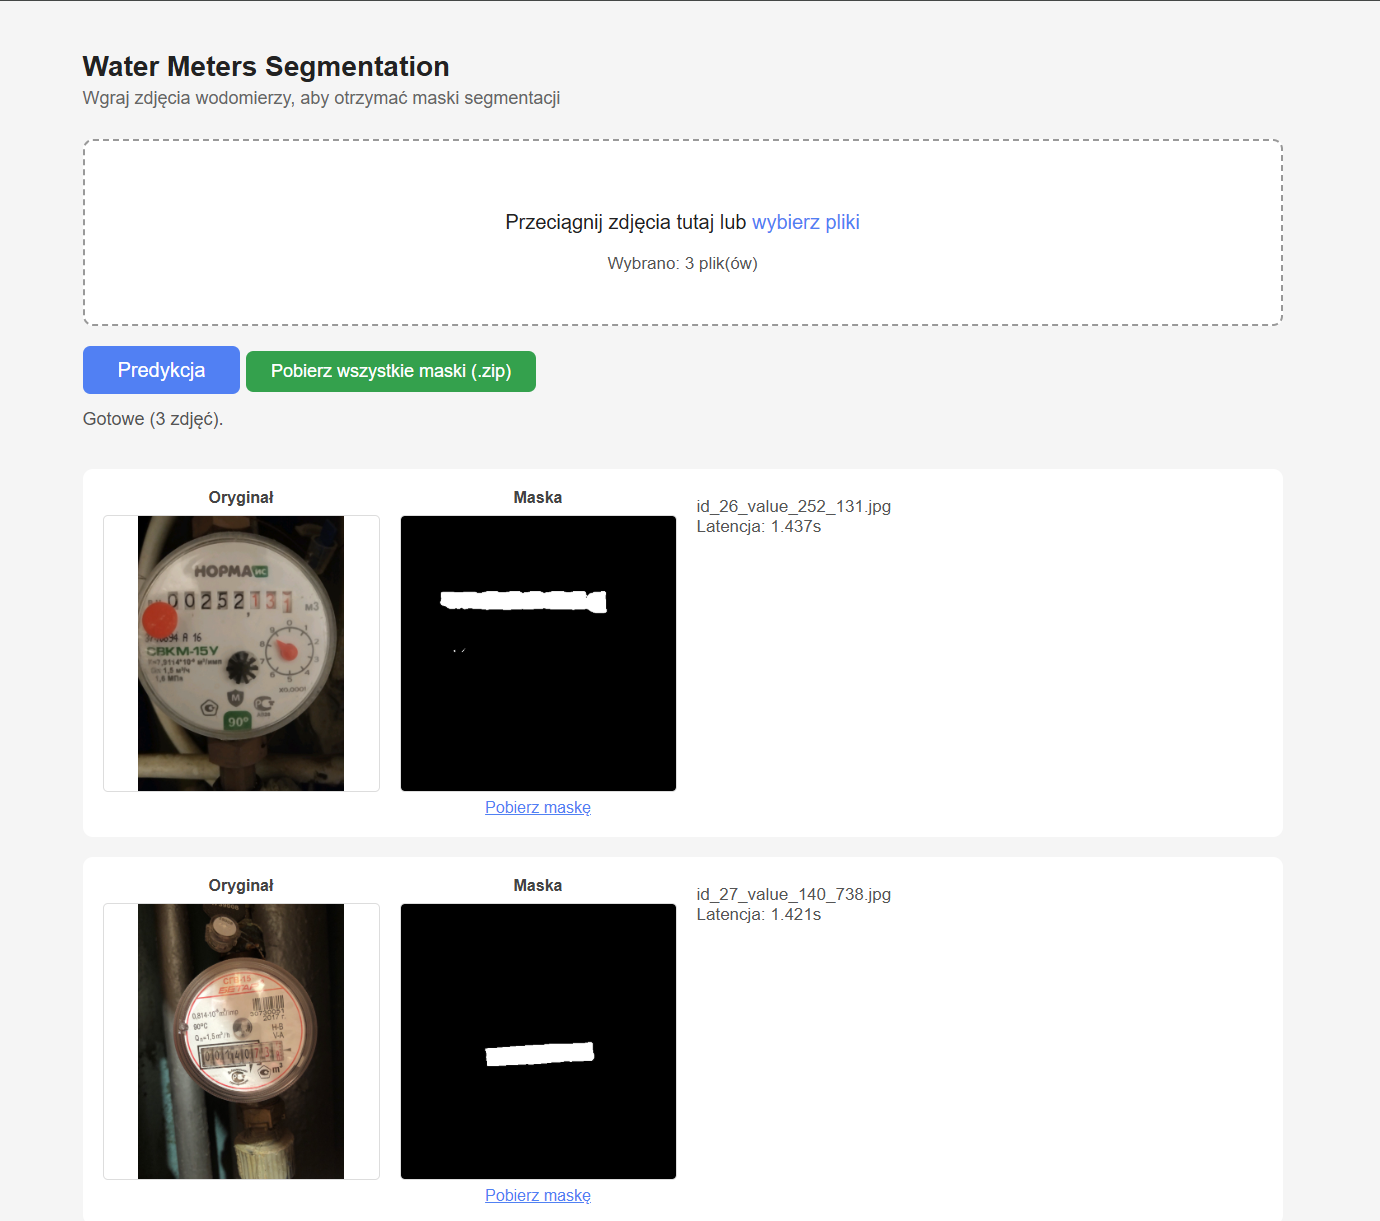
\includegraphics[width=\linewidth]{img/06_wdrozenie_systemu/deployed_app.png}
  \caption{Działający interfejs webowy API modelu: segmentacja trzech zdjęć wodomierzy z wygenerowanymi maskami i zmierzoną latencją predykcji}
  \label{fig:deployed-app}
\end{figure}

Po zakończeniu pracy należy ponownie uruchomić \textit{Manual EC2 Control} z akcją \textit{stop}, aby nie generować zbędnych kosztów.

\subsubsection{Scenariusz 3: Lokalna predykcja (wyłącznie dla deweloperów)}

Predykcję można uruchomić lokalnie bez infrastruktury chmurowej. Opcja ta wymaga jednak spełnienia warunków niedostępnych dla typowego użytkownika końcowego.

Wymagania wstępne:
\begin{itemize}
  \item działająca instancja EC2 z MLflow (model musi być zarejestrowany w stadium Production),
  \item lokalne poświadczenia AWS skonfigurowane w \texttt{\textasciitilde/.aws/credentials}: \texttt{AWS\_ACCESS\_KEY\_ID}, \texttt{AWS\_SECRET\_ACCESS\_KEY}, \texttt{AWS\_SESSION\_TOKEN},
  \item Python z zależnościami projektu zainstalowanymi lokalnie.
\end{itemize}

Przy spełnieniu powyższych warunków predykcja przebiega następująco:
\begin{enumerate}
  \item Pobranie modelu Production z MLflow na dysk lokalny:
        \begin{lstlisting}[numbers=none,frame=none,backgroundcolor=\color{white},basicstyle=\ttfamily\small,xleftmargin=0pt]
python WMS/scripts/sync_model_aws.py
\end{lstlisting}
  \item Umieszczenie obrazów do segmentacji w \texttt{WMS/data/predict/input/}.
  \item Uruchomienie predykcji: \texttt{python WMS/src/predicts.py}
  \item Wyniki zapisywane są w \texttt{WMS/data/predict/output/}.
\end{enumerate}

Poświadczenia AWS w środowisku AWS Academy są tymczasowe (ważność 4~godziny) i wymagają ręcznego odnawiania przy każdej sesji laboratoryjnej. Z tego powodu opcja lokalnej predykcji jest praktycznie dostępna wyłącznie dla operatora posiadającego bezpośredni dostęp do konta AWS, a nie dla użytkownika końcowego.

Opisane scenariusze pokrywają wszystkie typowe przypadki interakcji z systemem.

\subsection{Dostępne operacje zarządzania wdrożeniem}

System udostępnia cztery workflow GitHub Actions do zarządzania infrastrukturą i wdrożeniami. Tabela~\ref{tab:workflows} zestawia je wraz z wyzwalaczami i przeznaczeniem.

\begin{table}[H]
\centering
\caption{Workflow GitHub Actions dostępne w systemie}
\label{tab:workflows}
\begin{tabular}{|p{4.2cm}|p{3.2cm}|p{6.5cm}|}
\hline
\textbf{Workflow} & \textbf{Wyzwalacz} & \textbf{Przeznaczenie} \\
\hline
\texttt{training-data-pipeline} & Push do \texttt{data/*}, \texttt{workflow\_dispatch} & Pełny pipeline: pobieranie danych z S3, walidacja, trening, bramka jakości. Jeśli model poprawił metryki: wdrożenie na k3s i scalenie PR. EC2 uruchamiany i zatrzymywany automatycznie. \\
\hline
\texttt{release-deploy} & Push do \texttt{main} (zmiany kodu/Docker/Helm), \texttt{workflow\_dispatch} & Wdrożenie modelu na klaster k3s bez treningu: build Docker, push do ECR, aktualizacja Helm. Używany przy zmianach kodu serwowania lub jako ręczne ponowne wdrożenie. EC2 uruchamiany i zatrzymywany automatycznie. \\
\hline
\texttt{ec2-manual-control} & Tylko \texttt{workflow\_dispatch} & Ręczne uruchomienie lub zatrzymanie instancji EC2. Po starcie wyświetla aktualne IP i URL MLflow w podsumowaniu. Używany gdy potrzebny jest dostęp do API lub interfejsu MLflow. \\
\hline
\texttt{deploy-model} & Reużywalny (\texttt{workflow\_call}), \texttt{workflow\_dispatch} & Właściwy krok wdrożenia wywoływany przez \texttt{training-data-pipeline} i \texttt{release-deploy}. Można też uruchomić samodzielnie. Działa na self-hosted runnerze EC2, uwierzytelniając się przez rolę IAM instancji. \\
\hline
\end{tabular}
\end{table}

Żaden z powyższych workflow nie wymaga lokalnych poświadczeń AWS na komputerze operatora. Workflow uruchamiane na runnerze \texttt{ubuntu-latest} (start/stop EC2) korzystają z sekretów repozytorium GitHub, natomiast \texttt{deploy-model} działa na self-hosted runnerze EC2 i uwierzytelnia się przez rolę IAM przypisaną do instancji.


\section{Analiza Wyników i Działania Systemu}
\label{sec:Analiza_wynikow}

\subsection{Cel analizy i kryteria oceny}

Rozdział ma charakter porównawczy i zestawia ze sobą dwa podejścia do rozwijania modelu AI: manualne oraz zautomatyzowane CI/CD.

Aby porównanie było jednoznaczne, analizę przeprowadzono w sześciu wymiarach:
\begin{itemize}
  \item nakład pracy człowieka i całkowity czas realizacji cyklu
  \item jakość modelu (Dice, IoU) i skuteczność bramki jakości,
  \item koszty infrastruktury,
  \item zużycie zasobów,
  \item ryzyko błędu ludzkiego
  \item skalowalność procesu.
\end{itemize}

\subsection{Metodologia porównania}

Porównano dwa scenariusze realizujące ten sam cel biznesowy (dodanie nowych danych i dostarczenie działającego modelu):
\begin{enumerate}
  \item \textbf{Podejście ręczne} --- inżynier ręcznie wykonuje kolejne kroki: walidację danych, trening, ocenę metryk, decyzję o promocji modelu i wdrożenie.
  \item \textbf{Podejście zautomatyzowane (zrealizowany pipeline)} --- operator dostarcza dane przez \texttt{git push}, a dalszy przebieg realizują skrypty i workflow.
\end{enumerate}

Utrzymanie porównywalnego środowiska narzędziowego w obu podejściach było kluczowe. Pozwala przypisać różnice w nakładzie pracy i ryzyku błędu automatyzacji procesu, a nie zmianie technologii. Dokładniejsze wskazanie granicy między podejściami ułatwia poniższe zestawienie:
\begin{itemize}
  \item \textbf{Narzędzia wspólne dla obu podejść:} EC2 (środowisko obliczeniowe), MLflow (śledzenie eksperymentów, metryk i wersji modeli), k3s z Helm (wdrożenie), Docker (konteneryzacja API).
  \item \textbf{Narzędzia wyłącznie dla podejścia zautomatyzowanego:} GitHub Actions (orkiestracja pipeline), DVC (wersjonowanie \textit{danych treningowych} i synchronizacja z S3), hook \texttt{pre-push} Git (automatyczne tworzenie gałęzi danych), Terraform (infrastruktura jako kod).
\end{itemize}

Porównanie obejmuje sześć wymiarów:
\begin{itemize}
  \item \textbf{Nakład pracy człowieka i czas całkowity} (podsekcja~\ref{subsec:czasy}),
  \item \textbf{Jakość modelu} (podsekcja~\ref{subsec:metryki}),
  \item \textbf{Koszty infrastruktury i obsługi} (podsekcja~\ref{subsec:koszty}),
  \item \textbf{Zużycie zasobów} (podsekcja~\ref{subsec:zasoby}),
  \item \textbf{Ryzyko błędu ludzkiego} (podsekcje~\ref{subsubsec:stabilnosc}).
  \item \textbf{skalowalność procesu} (podsekcje~\ref{subsubsec:skalowalnosc}).
\end{itemize}

\textbf{Istotne ograniczenie metodologiczne:} czasy dla podejścia ręcznego mają charakter szacunkowy i zostały określone na podstawie doświadczeń zdobytych podczas realizacji projektu oraz analizy poszczególnych etapów procesu. Czasy podejścia zautomatyzowanego pochodzą z logów GitHub Actions i stanowią rzeczywisty pomiar czasu wykonania.

\subsection{Czasy wykonania i nakład pracy człowieka}
\label{subsec:czasy}

\begin{table}[H]
\centering
\caption{Porównanie nakładu pracy człowieka i czasu realizacji cyklu}
\label{tab:czasy}
\begin{tabular}{|l|r|r|}
\hline
\textbf{Etap} & \textbf{Ręczny} & \textbf{Zautomatyzowane CI/CD} \\
\hline
Przygotowanie i upload danych & $\sim$30 min & $\sim$10 min \\
Walidacja danych & $\sim$30 min & automatyczna \\
Trening modelu & $\sim$3 h & automatyczny \\
Ocena jakości i decyzja wdrożeniowa & $\sim$15 min & automatyczna \\
Wdrożenie & $\sim$45 min & automatyczne \\
\hline
\textbf{Nakład człowieka łącznie} & $\sim$5 h & $\sim$20 min \\
\textbf{Całkowity czas cyklu} & $\sim$5 h & $\sim$4 h \\
\hline
\end{tabular}
\end{table}

Wynik oznacza redukcję aktywnego czasu inżyniera o około \textbf{93\%} (z 300 min do 20 min) na jeden cykl. Jednocześnie całkowity czas cyklu został skrócony o około \textbf{20\%}, ponieważ głównym składnikiem pozostaje sam trening modelu. Zakładając pewną niedokładność oszacowań, wyniki nadal pozostają jednoznaczne: automatyzacja znacząco redukuje nakład pracy człowieka i skraca czas realizacji procesu.

Kluczowe jest rozróżnienie między \textbf{nakładem pracy człowieka} a \textbf{całkowitym czasem realizacji}. W podejściu ręcznym obie wartości są praktycznie tożsame, ponieważ operator uczestniczy we wszystkich etapach. W podejściu zautomatyzowanym człowiek dostarcza dane, a następnie pipeline działa bez jego udziału co jest ogromną zaletą dla podejścia zautomatyzowanego.

W praktyce ta różnica może się dodatkowo powiększyć przez fakt, że cykl manualny obejmuje kilkanaście interwencji: uruchomienie środowiska, trening, monitorowanie logów, ocenę metryk, rejestrację modelu, aktualizację konfiguracji wdrożenia i weryfikację działania po deploymencie. Każdy etap jest potencjalnym źródłem błędu. W pipeline CI/CD większość tych kroków jest wykonywana automatycznie i audytowalnie.

\subsection{Jakość modeli i skuteczność bramki jakości}
\label{subsec:metryki}

Poniższe wykresy i tabela nr~\ref{tab:metryki} przedstawiają metryki zarejestrowane w MLflow dla kolejnych wersji modelu.

\begin{figure}[H]
 \centering
 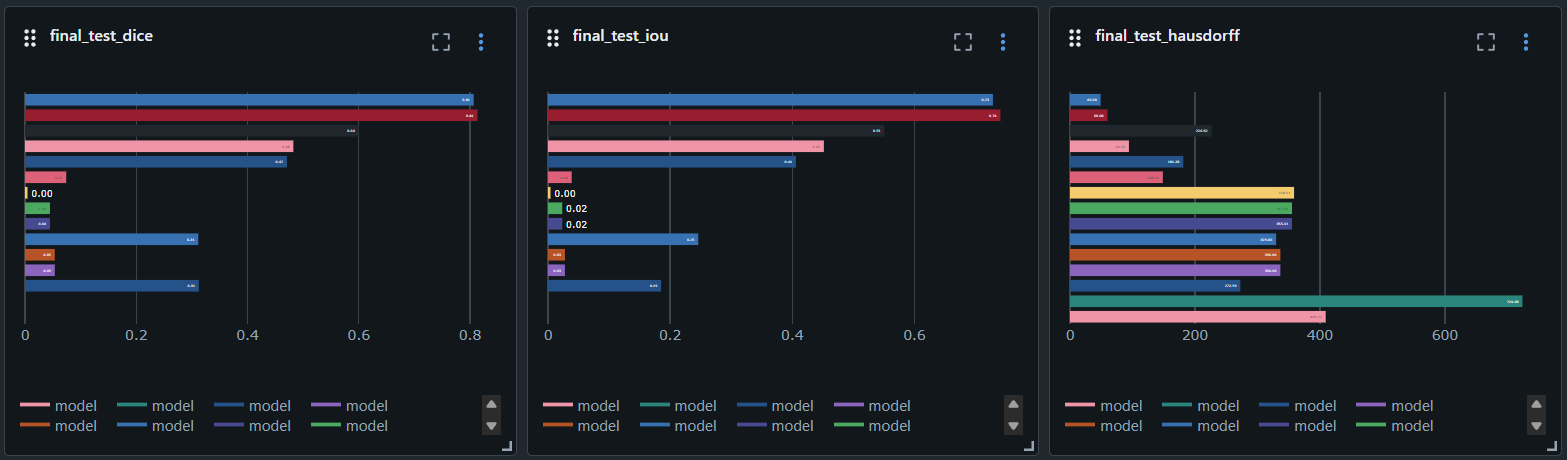
\includegraphics[width=\linewidth]{img/07_analiza_wynikow_i_dzialanie_systemu/mlfow_models_metrics_all.png}
 \caption{Metryki jakości modelu w interfejsie MLflow}
 \label{fig:mlflow-metrics-all}
\end{figure}

\begin{table}[H]
\centering
\caption{Metryki jakości modelu dla kolejnych wersji}
\label{tab:metryki}
\begin{tabular}{|l|c|c|c|}
\hline
\textbf{Wersja modelu} & \textbf{Dice} & \textbf{IoU} & \textbf{Hausdorff} \\
\hline
v21  & 0{,}8067 & 0{,}7286 & 49{,}0034 \\
v20  & 0{,}8134 & 0{,}7409 & 59{,}9987 \\
v18  & 0{,}5998 & 0{,}5508 & 226{,}5247 \\
v16  & 0{,}4825 & 0{,}4518 & 94{,}3321 \\
v14  & 0{,}4710 & 0{,}4060 & 181{,}2840 \\
v13  & 0{,}0741 & 0{,}0388 & 148{,}5599 \\
v12  & 0{,}0042 & 0{,}0021 & 358{,}6141 \\
v11  & 0{,}0449 & 0{,}0233 & 355{,}3105 \\
v10  & 0{,}0449 & 0{,}0233 & 355{,}3105 \\
v9   & 0{,}3116 & 0{,}2461 & 329{,}8586 \\
v8   & 0{,}0536 & 0{,}0278 & 336{,}6613 \\
v7   & 0{,}0536 & 0{,}0278 & 336{,}6613 \\
v5   & 0{,}3125 & 0{,}1852 & 272{,}5949 \\
v3   & $3{,}5689\cdot 10^{-10}$ & $3{,}5689\cdot 10^{-10}$ & 724{,}0773 \\
v1   & $3{,}5386\cdot 10^{-10}$ & $3{,}5386\cdot 10^{-10}$ & 409{,}2163 \\
\hline
\end{tabular}
\end{table}

Dane przedstawione w powyższej tabeli wskazują, że wszystkie modele były poprawnie rejestrowane niezależnie od osiągniętych metryk jakościowych.

\begin{table}[H]
\centering
\caption{Wersje modelu awansowane do etapu Production}
\label{tab:metryki-production}
\begin{tabular}{|l|c|c|c|}
\hline
\textbf{Wersja modelu} & \textbf{Dice} & \textbf{IoU} & \textbf{Hausdorff} \\
\hline
v20  & 0{,}8134 & 0{,}7409 & 59{,}9987 \\
v18  & 0{,}5998 & 0{,}5508 & 226{,}5247 \\
v16  & 0{,}4825 & 0{,}4518 & 94{,}3321 \\
v14  & 0{,}4710 & 0{,}4060 & 181{,}2840 \\
v9   & 0{,}3116 & 0{,}2461 & 329{,}8586 \\
v5   & 0{,}3125 & 0{,}1852 & 272{,}5949 \\
v3   & $3{,}5689\cdot 10^{-10}$ & $3{,}5689\cdot 10^{-10}$ & 724{,}0773 \\
v1   & $3{,}5386\cdot 10^{-10}$ & $3{,}5386\cdot 10^{-10}$ & 409{,}2163 \\
\hline
\end{tabular}
\end{table}

\begin{figure}[H]
 \centering
 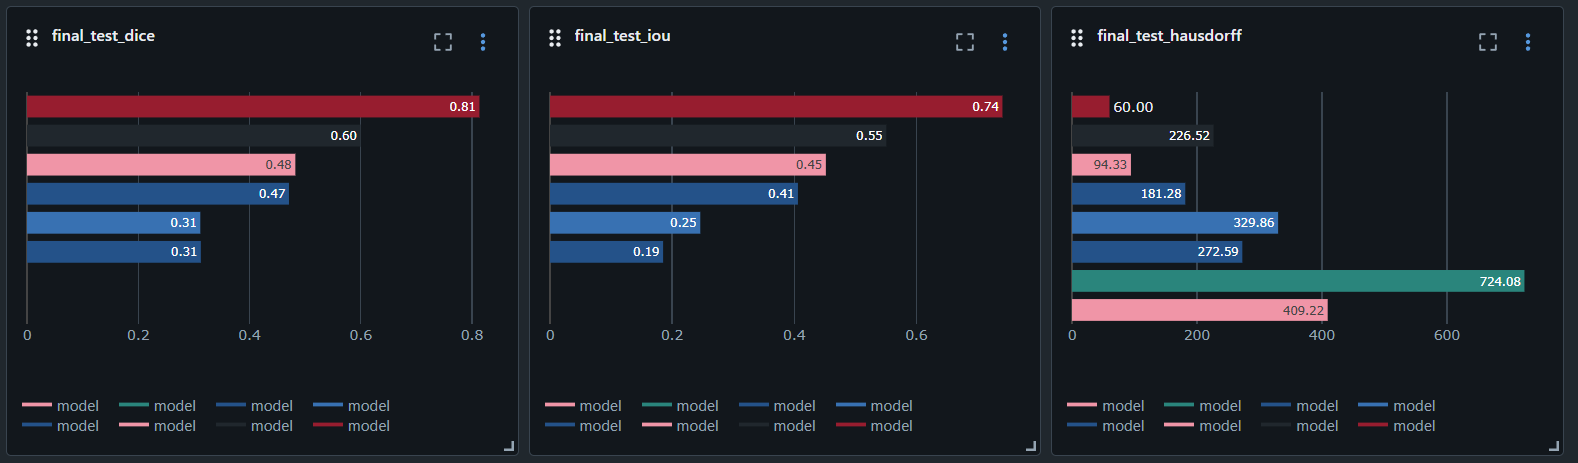
\includegraphics[width=\linewidth]{img/07_analiza_wynikow_i_dzialanie_systemu/mlflow_models_metrics_production.png}
 \caption{Rejestr modeli MLflow --- widok wersji ze stadium Production}
 \label{fig:mlflow-metrics-production}
\end{figure}
\mbox{}\\
Analiza całego zbioru wersji potwierdza poprawność mechanizmu kontroli jakości. Wszystkie przebiegi zostały zarejestrowane, natomiast do etapu \textit{Production} awansowały wyłącznie wersje spełniające kryteria bramki. Pozostałe wersje nie uczestniczyły we wdrożeniu produkcyjnym.

Warto podkreślić, że bardzo wczesne wersje modelu (v1 i v3) uzyskały wartości Dice/IoU rzędu \(10^{-10}\), co praktycznie oznacza brak użytecznej zdolności predykcyjnej. Tak skrajne wartości bywają słabo widoczne na wykresach, ponieważ warstwa wizualizacji skaluje osie pod wartości dominujące. Nie jest to błąd eksperymentu ani logowania metryk; wartości są poprawnie zarejestrowane w widoku tabelarycznym MLflow.

Najlepszy model (v20) osiągnął Dice 0{,}8134 i IoU 0{,}7409. Wynik jest niższy od modelu referencyjnego (Dice 0{,}9275, IoU 0{,}8865), co wynika ze świadomie przyjętego ograniczenia czasu treningu i budżetu. Celem projektu była walidacja procesu automatycznego utrzymania i kontrolowanej promocji modeli, a nie maksymalizacja metryk absolutnych.

W porównaniu z podejściem manualnym przyjęto konserwatywne założenie, że wszystkie wyniki uzyskane w pipeline CI/CD są osiągalne również ręcznie. Jednocześnie podejście ręczne daje większą swobodę uruchamiania dłuższych treningów i trenowania na większych zbiorach bez narzutu pełnej orkiestracji procesu. Oznacza to, że w wymiarze czysto modelowym (bez uwzględnienia ryzyka operacyjnego i kosztu pracy człowieka) podejście manualne może prowadzić do szybszego dojścia do wysokich metryk, w tym do poziomu zbliżonego do repozytorium referencyjnego przy wykorzystaniu pełnego zbioru danych.

\begin{figure}[H]
 \centering
 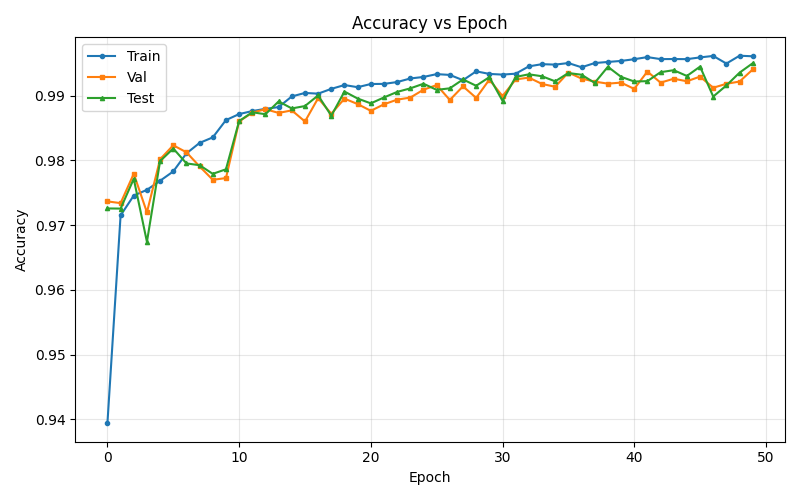
\includegraphics[width=0.85\linewidth]{img/07_analiza_wynikow_i_dzialanie_systemu/plot_accuracy.png}
 \caption{Wykres metryki Accuracy dla najlepszej wersji modelu (v20)}
 \label{fig:mlflow-accuracy}
\end{figure}

Metryka Accuracy rośnie szybko i stabilizuje się na poziomie powyżej 0{,}99 dla wszystkich podzbiorów. W zadaniu segmentacji binarnej jest to jednak metryka pomocnicza, ponieważ może zawyżać ocenę jakości przy dominacji klasy tła.

\begin{figure}[H]
 \centering
 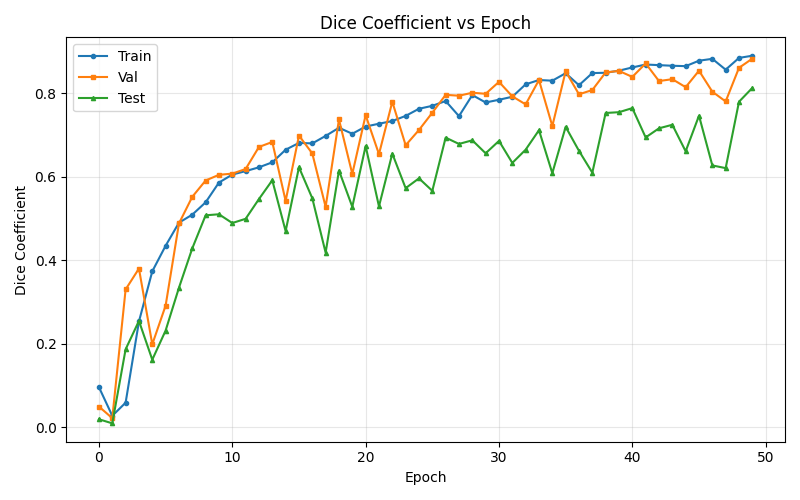
\includegraphics[width=0.80\linewidth]{img/07_analiza_wynikow_i_dzialanie_systemu/plot_dice.png}
 \caption{Wykres metryki Dice dla najlepszej wersji modelu (v20)}
 \label{fig:mlflow-dice}
\end{figure}

Współczynnik Dice, kluczowy dla segmentacji, wykazuje systematyczny wzrost w trakcie uczenia i osiąga wysokie wartości końcowe. Niewielki odstęp między przebiegami treningowym i walidacyjnym wskazuje na dobrą generalizację modelu.

\begin{figure}[H]
 \centering
 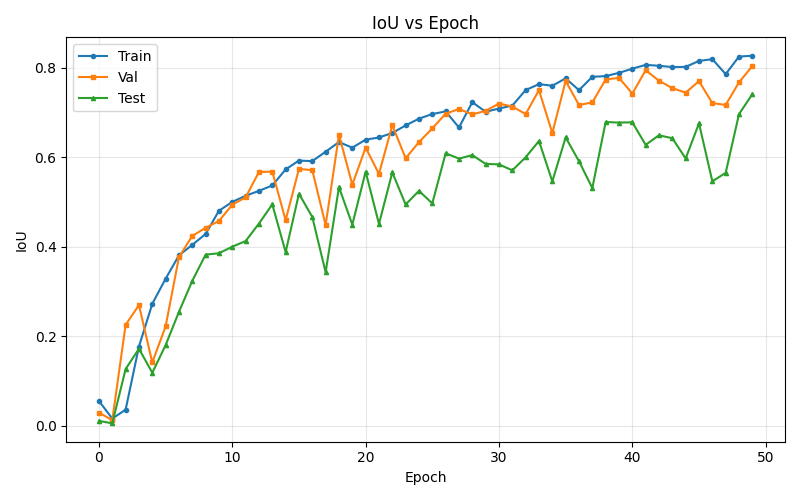
\includegraphics[width=0.85\linewidth]{img/07_analiza_wynikow_i_dzialanie_systemu/plot_iou.png}
 \caption{Wykres metryki IoU dla najlepszej wersji modelu (v20)}
 \label{fig:mlflow-iou}
\end{figure}

Metryka IoU zachowuje trend zgodny z Dice: wyraźnie rośnie wraz z kolejnymi epokami i stabilizuje się pod koniec treningu. Końcowe wartości potwierdzają satysfakcjonującą zgodność predykowanych masek z maskami referencyjnymi.

\begin{figure}[H]
 \centering
 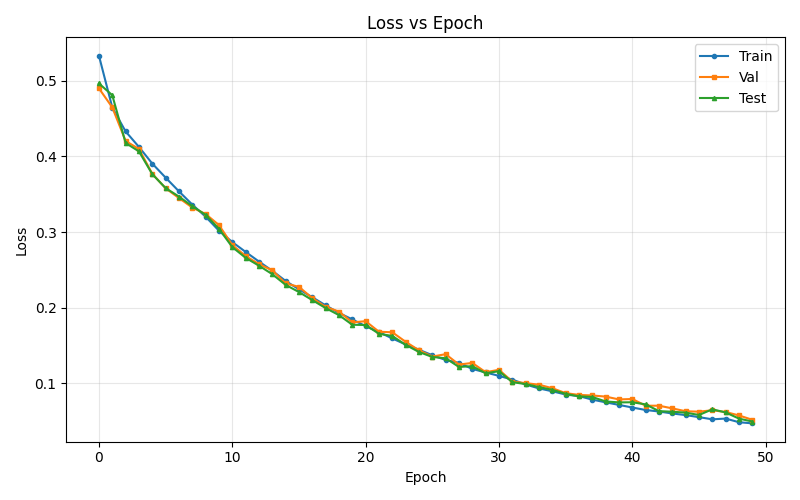
\includegraphics[width=\linewidth]{img/07_analiza_wynikow_i_dzialanie_systemu/plot_loss.png}
 \caption{Wykres funkcji straty dla najlepszej wersji modelu (v20)}
 \label{fig:mlflow-loss}
\end{figure}

Funkcja straty maleje monotonicznie dla zbioru treningowego, walidacyjnego i testowego, bez oznak niestabilności. Taki przebieg potwierdza poprawną zbieżność procesu uczenia i brak wyraźnych symptomów przeuczenia.

\begin{figure}[H]
 \centering
 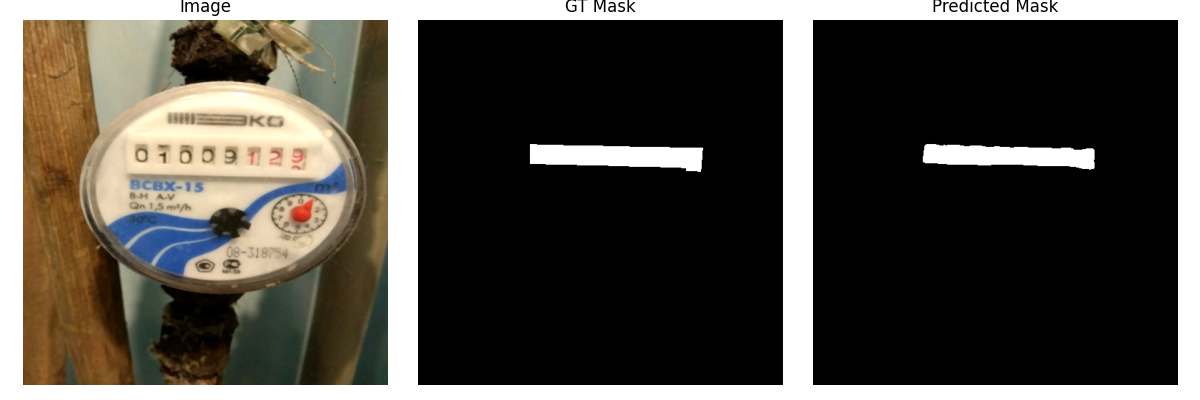
\includegraphics[width=\linewidth]{img/07_analiza_wynikow_i_dzialanie_systemu/plot_pred_2.png}
 \caption{Przykład predykcji modelu v20 (wejście, maska referencyjna, maska przewidywana)}
 \label{fig:mlflow-pred-2}
\end{figure}

\subsection{Koszty infrastruktury}
\label{subsec:koszty}

Analiza kosztowa została zweryfikowana z wykorzystaniem oficjalnego cennika AWS (Price List API) dla regionu \texttt{us-east-1}, stan na luty 2026~\cite{aws_pricing}. Tabela~\ref{tab:koszty-cennik} przedstawia stawki jednostkowe użyte do obliczeń.

\begin{table}[H]
\centering
\caption{Stawki jednostkowe AWS użyte w analizie kosztów}
\label{tab:koszty-cennik}
\begin{tabular}{|p{5.2cm}|p{2.1cm}|p{6.7cm}|}
\hline
\textbf{Pozycja} & \textbf{Stawka} & \textbf{Źródło i uwagi} \\
\hline
EC2 \texttt{t3.large} Linux On-Demand & \$0{,}0832/h & AmazonEC2 Price List API, US East (N. Virginia) \\
\hline
EBS \texttt{gp3} & \$0{,}08/GB-mies. & AmazonEC2 Price List API (wolumen systemowy EC2) \\
\hline
S3 Standard storage & \$0{,}023/GB-mies. & AmazonS3 Price List API, pierwszy próg do 50~TB \\
\hline
S3 PUT/COPY/POST/LIST & \$0{,}005/1000 req. & AmazonS3 Price List API \\
\hline
S3 GET/pozostałe & \$0{,}004/10000 req. & AmazonS3 Price List API \\
\hline
ECR private storage & \$0{,}10/GB-mies. & AmazonECR Price List API \\
\hline
\end{tabular}
\end{table}

Do oszacowania kosztu miesięcznego przyjęto realistyczny profil użytkowania środowiska:
\begin{itemize}
  \item 30~GB wolumenu EBS \texttt{gp3} dla instancji,
  \item 20~GB danych i artefaktów w S3,
  \item 1{,}5~GB obrazów kontenerowych w ECR,
  \item 5000 operacji S3 typu PUT/LIST i 30000 operacji GET miesięcznie,
  \item pojedynczy cykl treningowy: 3{,}5~h pracy EC2.
\end{itemize}

Koszt pojedynczego cyklu obliczeniowego wynosi:
\[
C_{cykl} = 3{,}5 \cdot 0{,}0832 = 0{,}2912\ \text{USD}.
\]

Koszt stały miesięczny (niezależny od liczby cykli) wynosi:
\[
C_{stały} = 30\cdot0{,}08 + 20\cdot0{,}023 + 1{,}5\cdot0{,}10 + \frac{5000}{1000}\cdot0{,}005 + \frac{30000}{10000}\cdot0{,}004 \approx 3{,}05\ \text{USD/mies.}
\]

Całkowity koszt miesięczny można więc zapisać jako:
\[
C_{mies}(N)=3{,}05 + 0{,}2912\cdot N,
\]
gdzie \(N\) oznacza liczbę pełnych cykli treningowych w miesiącu.

\begin{table}[H]
\centering
\caption{Koszt miesięczny dla różnych intensywności użycia pipeline CI/CD}
\label{tab:koszty-scenariusze}
\begin{tabular}{|c|c|c|}
\hline
\textbf{Liczba cykli/mies.} & \textbf{Koszt zmienny EC2} & \textbf{Koszt całkowity} \\
\hline
10 & \$2{,}91 & \$5{,}96 \\
\hline
30 & \$8{,}74 & \$11{,}79 \\
\hline
60 & \$17{,}47 & \$20{,}52 \\
\hline
\end{tabular}
\end{table}

\textbf{Koszt wdrożenia automatyzacji i porównanie z obsługą manualną (PLN).}
Do analizy doliczono jednorazowy koszt przygotowania infrastruktury automatycznej:
\[
C_0 = 10000\ \text{PLN}.
\]

W podejściu manualnym przyjęto, że utrzymanie procesu zajmuje \textbf{20\% czasu pracy inżyniera} (0,2 etatu). Dla miesięcznej pensji brutto \(P\) koszt pracy manualnej wynosi:
\[
C_{\text{manual,praca}} = 0{,}2\cdot P.
\]

Z pomiarów czasu (5 h manualnie vs 20 min w CI/CD) wynika, że obciążenie człowieka po automatyzacji to około \(6{,}67\%\) obciążenia manualnego. Stąd:
\[
C_{\text{CI/CD,praca}} \approx 0{,}0133\cdot P.
\]

Miesięczna różnica kosztu pracy:
\[
\Delta C_{\text{praca}} = (0{,}2 - 0{,}0133)\cdot P = 0{,}1867\cdot P.
\]

Czas zwrotu jednorazowego kosztu wdrożenia:
\[
T_{\text{BE}} = \frac{C_0}{\Delta C_{\text{praca}}}
= \frac{10000}{0{,}1867\cdot P}\ \text{[mies.]}.
\]

\begin{table}[H]
\centering
\caption{Próg opłacalności automatyzacji dla różnych pensji miesięcznych}
\label{tab:break-even-pln}
\begin{tabular}{|c|c|c|c|}
\hline
\textbf{Pensja \(P\) [PLN/mies.]} & \textbf{Manual \(0{,}2P\)} & \textbf{CI/CD \(0{,}0133P\)} & \textbf{Zwrot \(T_{\text{BE}}\)} \\
\hline
8000  & 1600 PLN/mies. & 106 PLN/mies. & 6{,}69 mies. \\
\hline
12000 & 2400 PLN/mies. & 160 PLN/mies. & 4{,}46 mies. \\
\hline
16000 & 3200 PLN/mies. & 213 PLN/mies. & 3{,}35 mies. \\
\hline
\end{tabular}
\end{table}

Wniosek z tej części analizy: nawet po doliczeniu jednorazowego kosztu 10000 PLN automatyzacja zwraca się względnie szybko względem stałego obciążenia pracy manualnej.

Wyniki pokazują, że automatyzacja CI/CD faktycznie przyspiesza pracę i redukuje nakład operacyjny człowieka, ale odbywa się to kosztem stałych i narastających kosztów chmurowych. W praktyce oznacza to, że podejście CI/CD jest \textbf{szybkie i efektywne operacyjnie}, lecz \textbf{kosztowne finansowo} przy większej liczbie iteracji oraz przy przejściu do architektury produkcyjnej o wyższych wymaganiach dostępności i bezpieczeństwa.

\subsection{Zużycie zasobów i działanie usługi}
\label{subsec:zasoby}

Serwis inferencyjny działa stabilnie na instancji \texttt{t3.large}. Model ładowany jest jednorazowo przy starcie kontenera, a monitorowane metryki API (liczba predykcji, opóźnienia, błędy) potwierdzają poprawne działanie wdrożenia. Dla przyjętej skali obciążenia zasoby CPU i RAM były wystarczające.

W kontekście obciążenia należy podkreślić, że projekt był testowany w skali laboratoryjnej, a nie pod pełnym ruchem produkcyjnym. Oznacza to, że sekcja zasobowa potwierdza wystarczalność środowiska dla przyjętego scenariusza, ale nie stanowi pełnego wyznacznika wydajnościowego dla skali wielokrotnie większej.

\subsection{Ocena jakościowa procesu}

\subsubsection{Łatwość wdrożenia}

Konfiguracja systemu wymagała jednorazowego, istotnego nakładu pracy: przygotowania Terraform, konfiguracji k3s i Helm, integracji MLflow z S3, implementacji walidacji danych i bramki jakości oraz przygotowania workflow GitHub Actions. Po wykonaniu tej inwestycji wejściowej kolejne iteracje procesu są realizowane z minimalną interwencją operatora.

Podejście ręczne nie ma kosztu wejścia na poziomie automatyzacji, ale generuje koszt powtarzalny przy każdym cyklu. Wraz ze wzrostem liczby iteracji rośnie obciążenie inżyniera oraz ryzyko błędu ludzkiego.

\subsubsection{Stabilność i podatność na błąd}
\label{subsubsec:stabilnosc}

W podejściu zautomatyzowanym trzy elementy istotnie ograniczają ryzyko błędu ludzkiego:
\begin{itemize}
  \item automatyczna walidacja danych wejściowych przed treningiem,
  \item automatyczna bramka jakości blokująca regresję modelu,
  \item automatyczne zatrzymanie EC2 po zakończeniu pipeline'u (także po błędzie).
\end{itemize}

W podejściu ręcznym wszystkie trzy decyzje pozostają po stronie operatora, co zwiększa prawdopodobieństwo przeoczeń i kosztownych pomyłek.

\begin{table}[H]
\centering
\caption{Porównanie ryzyka operacyjnego: manual vs CI/CD}
\label{tab:ryzyko-porownanie}
\begin{tabular}{|p{4.3cm}|p{5.1cm}|p{5.1cm}|}
\hline
\textbf{Obszar ryzyka} & \textbf{Podejście ręczne} & \textbf{CI/CD} \\
\hline
Walidacja danych & zależna od dyscypliny operatora, ryzyko pominięcia błędnych próbek & automatyczna bramka QA blokująca dalszy pipeline \\
\hline
Decyzja o promocji modelu & ręczna interpretacja metryk, podatność na presję czasu & obiektywne kryterium bramki jakości (Dice/IoU) \\
\hline
Koszt chmury po awarii procesu & ryzyko pozostawienia uruchomionej instancji & automatyczne \texttt{stop-infra} po błędzie (\texttt{always()}) \\
\hline
Odtwarzalność eksperymentu & wymaga ręcznej dokumentacji i dyscypliny & logi workflow + MLflow + DVC zapewniają ślad audytowy \\
\hline
\end{tabular}
\end{table}

\subsubsection{Skalowalność}
\label{subsubsec:skalowalnosc}

Najważniejsza przewaga automatyzacji dotyczy skalowalności pracy zespołu: wzrost liczby iteracji nie zwiększa nakładu pracy człowieka proporcjonalnie do liczby cykli. Ograniczenia obecnej implementacji (single-node k3s, jeden runner, środowisko AWS Academy) mają charakter infrastrukturalny i budżetowy, nie logiczny. Logika pipeline'u może być przeniesiona do większego środowiska bez zmiany modelu procesu.

\begin{table}[H]
\centering
\caption{Skalowalność nakładu pracy człowieka przy wzroście liczby cykli}
\label{tab:skalowalnosc-pracy}
\begin{tabular}{|c|c|c|}
\hline
\textbf{Liczba cykli / mies.} & \textbf{Manual (5 h/cykl)} & \textbf{CI/CD (20 min/cykl)} \\
\hline
10 & 50 h & 3 h 20 min \\
\hline
30 & 150 h & 10 h \\
\hline
60 & 300 h & 20 h \\
\hline
\end{tabular}
\end{table}

Zestawienie to pokazuje, że przy wzroście liczby iteracji różnica obciążenia człowieka rośnie liniowo i szybko staje się kluczowym argumentem organizacyjnym na rzecz automatyzacji.

\section{Podsumowanie i wnioski WIP}
\label{sec:Podsumowanie}

\subsection{Realizacja celów pracy}

Niniejsza praca stawiała sobie za cel zaprojektowanie, implementację i ocenę zautomatyzowanego pipeline CI/CD dla modeli uczenia maszynowego. Poniżej zestawiono cele sformułowane we wprowadzeniu z oceną stopnia ich realizacji.

\begin{itemize}
  \item \textbf{Zaprojektowanie architektury systemu automatyzacji} --- % [UZUPEŁNIĆ: ocena realizacji]
  \item \textbf{Implementacja pipeline CI/CD integrującego walidację danych, trening i wdrożenie} --- % [UZUPEŁNIĆ: ocena realizacji]
  \item \textbf{Wprowadzenie obiektywnej bramki jakości opartej na metrykach ML} --- % [UZUPEŁNIĆ: ocena realizacji]
  \item \textbf{Porównanie podejścia ręcznego z zautomatyzowanym} --- % [UZUPEŁNIĆ: ocena realizacji]
  \item \textbf{Realizacja w ramach budżetu AWS Academy ($\sim$\$50)} --- % [UZUPEŁNIĆ: ostateczny koszt]
\end{itemize}

\subsection{Wnioski}

Na podstawie przeprowadzonych eksperymentów i obserwacji sformułowano następujące wnioski. Kontekst porównawczy oparty jest na literaturze z zakresu DevOps \cite{humble2010continuous} oraz MLOps \cite{kreuzberger2023mlops}.

\begin{enumerate}
  \item Automatyzacja pipeline CI/CD dla modeli ML istotnie skraca czas potrzebny do wdrożenia nowej wersji modelu w porównaniu do podejścia ręcznego. % [UZUPEŁNIĆ: konkretne liczby z eksperymentów]

  \item Wprowadzenie dynamicznej bramki jakości opartej na metrykach MLflow eliminuje ryzyko przypadkowego wdrożenia modelu gorszego od aktualnie produkcyjnego, co jest szczególnie istotne przy niedeterministycznym procesie trenowania.

  \item Wersjonowanie danych za pomocą DVC \cite{dvc_docs} zapewnia pełną odtwarzalność eksperymentów --- dla dowolnej wersji modelu możliwe jest odtworzenie dokładnego zbioru danych, na którym był trenowany.

  \item Zastosowanie k3s zamiast zarządzanego Kubernetes (EKS) okazało się wystarczające dla projektu proof of concept i pozwoliło znacząco ograniczyć koszty infrastruktury.

  \item Architektura stop/start instancji EC2 jest efektywna kosztowo, ale wprowadza opóźnienie na uruchomienie instancji i runnera ($\sim$3--5 minut). W środowisku produkcyjnym z wymaganiami SLA należałoby rozważyć utrzymywanie instancji aktywnej.
\end{enumerate}

\subsection{Ograniczenia}

Projekt realizowany był jako proof of concept z następującymi świadomymi ograniczeniami:

\begin{itemize}
  \item \textbf{Budżet AWS Academy} --- sesje laboratoryjne wygasają co 4 godziny, IAM role mają ograniczone uprawnienia (m.in. brak \texttt{s3:PutObject} dla lokalnych poświadczeń). Wymusiło to przeniesienie wszystkich operacji S3 do GitHub Actions.
  \item \textbf{Single-node k3s} --- brak wysokiej dostępności. Awaria instancji EC2 powoduje niedostępność całego systemu.
  \item \textbf{Mały zbiór danych} --- eksperyment przeprowadzono na zbiorze % [UZUPEŁNIĆ: liczba] obrazów. Zachowanie systemu przy znacznie większych zbiorach nie było testowane.
  \item \textbf{Jeden model} --- architektura jest zaprojektowana pod konkretny model (U-Net dla segmentacji). Generalizacja na inne typy modeli wymagałaby modyfikacji skryptów walidacji i bramki jakości.
\end{itemize}

\subsection{Kierunki dalszego rozwoju}

System stanowi solidną bazę, którą można rozbudować w kilku kierunkach:

\begin{itemize}
  \item \textbf{Multi-node Kubernetes} --- zastąpienie single-node k3s klastrem zapewniającym wysoką dostępność i możliwość skalowania poziomego.
  \item \textbf{Experiment tracking} --- rozbudowa wykorzystania MLflow o śledzenie hiperparametrów i automatyczne porównywanie wielu eksperymentów.
  \item \textbf{Data drift monitoring} --- dodanie mechanizmu wykrywającego rozbieżność między danymi treningowymi a produkcyjnymi.
  \item \textbf{A/B testing} --- wdrożenie mechanizmu stopniowego rollout nowej wersji modelu z automatycznym rollback przy pogorszeniu metryk.
  \item \textbf{Generalizacja} --- abstrakcja pipeline pod inne typy modeli i zadań ML, nie tylko segmentację obrazów.
\end{itemize}


\addcontentsline{toc}{section}{\refname}
\bibliographystyle{plainnat}
{\sloppy\bibliography{bibliografia}}
\end{document}
